\chapter{Neural networks}\label{chap:3}

\section{Neural Networks (da RICONTROLLARE DIDO)}
\subsection{Introduction}
Neural networks have lot of practical application but also they have been built to mimic the behaviour of a neuron in the brain.
A neuron is connecting a certain number of entries with other neuron though the synaptic junction.
The mapping between neuron is \textbf{non-linear}, and this is because the synaptic junction is passing information to other neuron only if the signal overcome a certain threshold.

The human brain is a strongly interconnected non-linear system of neurons:
in the human cortex there are $150\cdot10^3$ neurons per $mm^2$ that correspond to about $3 \cdot 10^3$ neurons. Each neuron has about $10^4$ synaptic connections and therefore the number of synaptic connection in the human brain is about $10^{15}$.
\begin{figure}[h!t]
\centering
\subfloat[][\emph{}]
{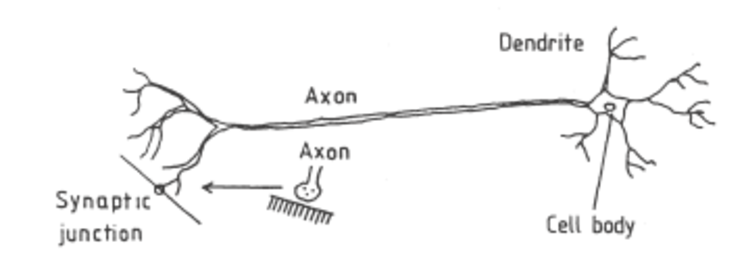
\includegraphics[width=.80\textwidth]{Immagini/Synaptic Junction.pdf}}
\caption{}
\end{figure}

Signal entering in the neuron are mixed together but the output signal is non linear, so to say, there is a filtering of the signal that is at the core of the process which through some parameters ensure that the neuron is performing well.
Both in nature and in artificial networks therefore there are parameters that need to be fixed (e.g. the threshold) to enhance the performance of the systems. But how do we manage to fix these parameters?
\paragraph{How neurons respond to stimulus: Hebb's Law}
 As originally postulated by Donald Hebb, the strength of a synaptic connection can be adjusted, if its level of activity changes. An active synapse, which repeatedly triggers the activation of its post-synaptic neuron, will grow in strength, while others will gradually weaken.
 In principle this is how in nature connection between neurons are created or destroyed. This can bee seen in figure \ref{fig:Arborization} which points out how links between neurons are strengthened or weakened in the previous years of brain life.
 \begin{figure}[h!t]
\centering
\subfloat[][\emph{}]
{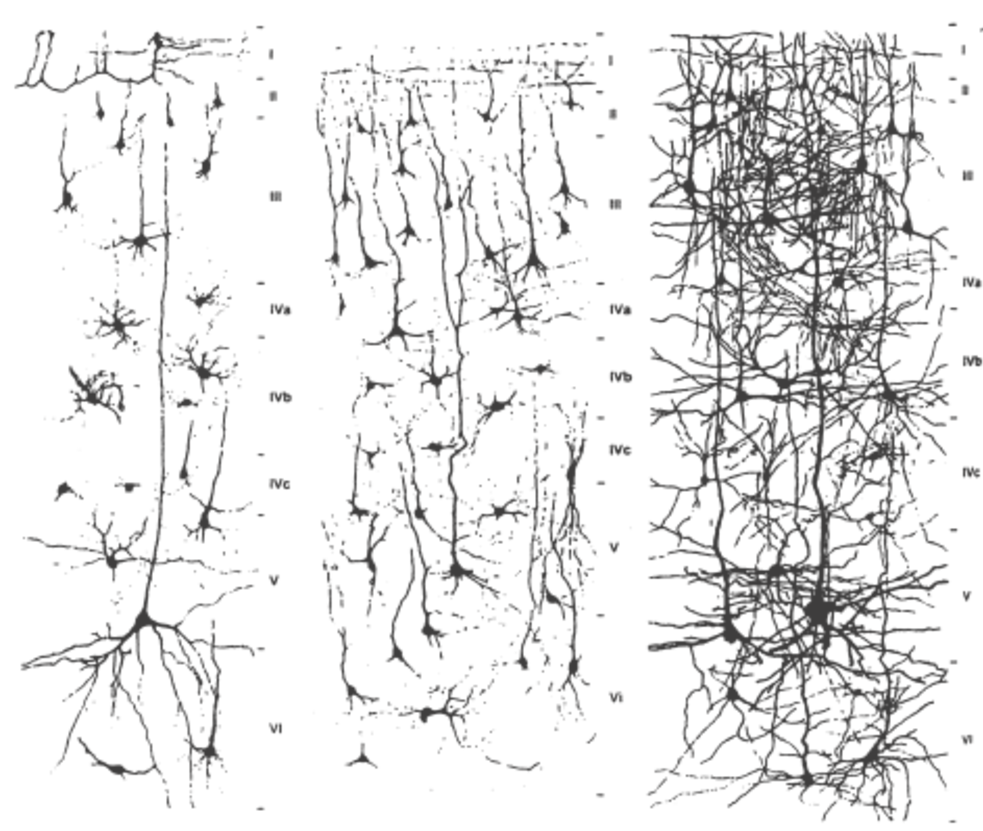
\includegraphics[width=.80\textwidth]{Immagini/DendriticHarborization.pdf}}
\caption {Development of dendritic arborization in the human visual cortex, from
(left) newborn, (middle) three-month-old, and (right) two-year-old infants }
\label{fig:Arborization}
\end{figure}


\paragraph{Brain size in animals:}
 Here it is important to relate the size of the brain to the total size of the animal. Studies in vertebrate animals have shown that the weight of the brain E grows with body weight P for species at a comparable level of evolution. Quantitatively, a quite strict relation of the form:
\begin{equation}
    Log(E)=a Log(p)+c
    \label{eq:RelationBrainSurface}
\end{equation}
with a $\sim 0.6$ was found. Since the surface of a body grows as $p=\frac{2}{3}$, one may suspect that the brain size grows in proportion to the body
surface, corresponding to the value $a = \frac{2}{3}$. This result is not too much of a
surprise, because the amount of external sensory information that the brain
has to process increases roughly in proportion to the surface of the body.
Vertebrates belonging to different levels of evolution differ, not so much in
the density of neurons, but in the magnitude of the constant of proportionality
C in the relation \ref{eq:RelationBrainSurface}.
To generalize this concept we can say that the size of the brain is scaling with the surface of the animals.

\subsection{Neural Network}\label{sec:ArtificialNeuralNetworks}
Neural network models are algorithms for cognitive tasks, such as learning and optimization, which are in a loose sense based on concepts derived from research into the nature of the brain (and thus related to the Hebb's law). In mathematical terms a neural network model is defined as a directed graph with the following properties: 
\begin{enumerate}
    \item A state variable $n_{i}$ is associated with each node $i$.
    \item A real-valued weight $w_{ik}$ is associated with each link ($ik$) between two nodes $i$ and $k$.
    \item A real-valued bias $\theta_{i}$ is associated with each node $i$.
    \item A transfer function $f(n_{k},w_{ik},\theta_i,(k\neq i)$ is defined, for each node $i$, which determines the state of the node as a function of its bias, of the weights of its incoming links, and of the states of the nodes connected to it by these links.
    
\end{enumerate}
In the standard terminology, the nodes are called neurons, the links are called synapses, and the bias is known as the activation threshold. The transfer function usually takes the form $f(\sum_{k}w_{ik}n_{k}-\theta_i)$, where $f(x)$ is either a discontinuous step function or its smoothly increasing generalization known as a sigmoidal function . Nodes without links toward them are called input neurons; output neurons are those with no link leading away from them. A feed-forward network is one whose topology admits no closed paths. It is our aim to study such models and learn what they can (and cannot) do.


In 1943 Warren McCulloch and Walter Pitts proposed general theory of information processing based on networks of binary switching or decision elements, which are somewhat euphemistically called "neurons", although they are far simpler than their real biological counterparts. Each one of these elements $i = 1, \dots , n$can only take the output values $n_{i} = 0,1$, where $n_i = 0$ represents the resting state and $n_i = 1$ the active state of the elementary unit.
In order to simulate the finite regenerative period of real neurons, changes in the state of the network are supposed to occur in discrete time steps $t = 0, 1,2, \dots$. The new state of a certain neural unit is determined by the influence of all other neurons, as expressed by a linear combination of their output values:

\begin{equation}
    h_{i}(t) = \sum_{j} w_{ij}n_{j}(t)
    \label{eq:ti}
\end{equation}
Here the matrix $w_{ij}$ represents the synaptic coupling strengths (or synaptic
efficacies) between neurons $j$ and $i$, while $h_i(t)$ models the total post-synaptic
potential at neuron $i$ caused by the action of all other neurons.
$h_i$ can be considered the input into the neural computing unit, and $n_i$ the
output. The properties of the neural network are completely determined by
the functional relation between hi(t) and $n_i(t + 1)$ . In the simplest case, the
neuron is assumed to become active if its input exceeds a certain threshold
$\theta_i$, which may well differ from one unit to the next. The \textbf{evolution of the
network} is then governed by the law

\begin{equation}
    n_{i}(t+1)=\Theta[ h_{i}(t)-\theta_{i}]
    \label{eq:ni}
\end{equation}
where $\Theta(x)$ is the unit step function.
 The network differs from a traditional computer in that the steps of the program are not executed sequentially, but in parallel within each elementary unit. One might say that the program code consists of a single statement, i.e. the combination of the
equations \ref{eq:ni} and \ref{eq:ti}. 
The extreme reduction of the program is compensated by the substitution of a vast number of processing elements ($10^{11}$ in the human brain!) for the single processing unit of a conventional, sequential electronic computer.

\subsubsection{Two simple model of neural network}

\paragraph{The perceptron}A perceptron is a specific type of neural network, but is actually a simplified model of the biological mechanisms of processing of sensory information, i.e. perception. In its simplest form, a perceptron consists of two separate layers of neurons 2 representing the input and output layer, respectively, as illustrated in Fig. \ref{fig:Simpleperceptron}. The neurons of the output layer receive synaptic signals from those of the input layer, but not vice versa, and the neurons within one layer do not communicate with each other. The flow of information is thus strictly directional; hence one speaks of a feed-forward network.
 \begin{figure}[h!t]
\centering
{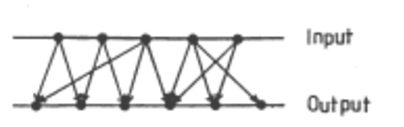
\includegraphics[width=.40\textwidth]{Immagini/SimplePerceptron.pdf}}
\caption {Simple perceptron, consisting of two layers of neurons. The input neurons feed into the neurons of the output layer, but not vice versa.}
\label{fig:Simpleperceptron}
\end{figure}

\paragraph{Ising model}
There is a similarity between a neural network of the type previously given and systems of elementary magnetic moments or spins, see
Fig. \ref{fig:Spinising}. 
In these systems, called Ising models, the spin $S_i$ at each lattice site $i$ can take only two different orientations, up or down, denoted by $S_i = +1$ (up) and $S_i = -1$ (down). The analogy to a neural network is realized by identifying each spin with a neuron and associating the upward orientation $S_i = + 1$ with the active state $n_i = 1$ and the downward orientation $S_i = -1$ with the resting state $n_i = O$.

 \begin{figure}[h!t]
\centering
{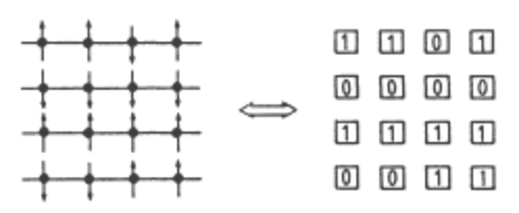
\includegraphics[width=.50\textwidth]{Immagini/SpinIsing.pdf}}
\caption {A one-to-one correspondence exists between lattices of magnetic spins with two different orientations (Ising systems) and McCulloch-Pitts neural networks. A spin pointing up (down) is identified with an active (resting) neuron.}
\label{fig:Spinising}
\end{figure}

These ideas were further developed by Little and Gordon Shaw
and by John Hopfield who studied how such a neural network or spin
system can store and retrieve information.

\paragraph{The Little and Hopfield models}
 The Little and Hopfield models differ in the manner in which the state of the system is updated. 
 \begin{itemize}
     \item  In Little's model all neurons (spins) are updated synchronously according to the law \ref{eq:ni}.
     \item  In the Hopfield model the neurons are updated sequentially one at a time (either in a certain fixed order or randomly). 
 \end{itemize}

 Sequential updating has a considerable advantage when the network is simulated on a conventional digital computer, and also for theoretical analysis of the properties of the network. On the other hand, it holds the essential conceptual disadvantage that the basic feature of neural networks, namely the simultaneous operation of a large number of parallel units, is given up. Neurons in the human brain surely do not operate sequentially, this being precisely the reason for the brain's superiority in complex tasks to even the fastest existing electronic computer.


\subsubsection{Associative memory}
Associative memory, i.e. storage and recall of information by association with
other information, may be the simplest application of "collective" computation on a neural network.

Here we define an associative memory as follows. Assume that p binary patterns containing N bits of information (i.e. p different images containing N bits for each), $\nu_{i}^{\mu}(i = 1, \dots , N;\mu=1,\dots,p)$, are stored in the to memory. If now a new pattern (not already memorized) $n_{i}$ is presented, that stored pattern $\nu_{i}^{\lambda}$ is to be recalled which most strongly resembles the presented pattern. This means that $\nu_{i}^{\lambda}$ and $n_{i}$ (which is the $i$\textsuperscript{th} bits of information of the new pattern) should differ in as few places as possible, i.e. that the mean square deviation 
 
\begin{equation}
    H_{\mu}=\sum_{i=1}^{N}(n_{i}-\nu_{i}^{\mu})^2
\end{equation}
is minimal for $\mu=\lambda$. $H_{\mu}$ is called the \textbf{Hamming distance} between the patterns $n_{i}$ and $\nu_{i}^{\mu}$.

In principle, this problem is easily solved on a standard digital computer by computing all values $H_{\mu}$ and then searching for the smallest one. However, if the memory contains many large patterns, this procedure can take quite a long time. We are therefore led to ask the question whether the patterns can be stored in a neural network of N elements (neurons) in such a way that the network evolves from the initial configuration $n_{i}$, corresponding to the presented pattern, into the desired configuration  $\nu_{i}^{\mu}$ under its own dynamics.

In order to formulate the problem, it is useful to invoke the analogy between neurons and Ising spins, mentioned before, replacing the quantities $\nu_{i}$, $n_i$ by new variables $s_{i}$, $\sigma_{i}$, which are defined as

\begin{equation}
\centering
    s_{i}=2n_{i}-1 \qquad \sigma_{i}=2\nu_{i}-1
\end{equation}
The new variables take the values $\pm1$, instead of 0 and 1 (remember that $n_{i}=0,1$). 
The squared deviations are then expressed as
\begin{equation}
    (n_{i}-\nu_{i}^{\mu})^2=\frac{1}{4}(s_{i}-\sigma_{i}^{\mu})^2=\frac{1}{4}(s_{i}^2-2 s_{i}\sigma_{i}^{\mu}+(\sigma_{i}^{\mu})^2)\underset{(\sigma_{i}^{\mu})^2=s_{i}^2=1}{=}\frac{1}{2}(1-s_{i}\sigma_{i}^{\mu})
\end{equation}
which gives a second expression for the Hamming distance in term of the new variables
\begin{equation}
     H_{\mu}=\sum_{i}\frac{1}{2}(1-s_{i}\sigma_{i}^{\mu})
\end{equation}
so $ H_{\mu}=0 \Leftrightarrow \forall i \quad s_{i}\sigma_{i}^{\mu}=1$ and thus \[s_{i}=\sigma_{i}^{\mu}\]

According to Hopfield the dynamical evolution of the state of the network is now defined as follows. The individual neurons $i$ are assigned new values $s_i(t + 1)$ in some randomly chosen sequence. The new values are computed according to the rule
\begin{equation}
    s_i(t + 1)=\sgn{\Big[\sum_{j=1}^{N}w_{ij}s_{j}(t)\Big]}
    \label{eq:evol}
\end{equation}
where the instantaneous output values of all neurons are to be taken on the right-hand side. The temporal evolution proceeds, as already mentioned in the previous chapter, in finite steps, i.e. $t$ takes only the discrete values $t = 0,1,2, \dots$. Equation \ref{eq:evol} corresponds to the rule \ref{eq:ni}, rewritten in the new variables $s_{i}$.


\subsubsection{Learning by Hebb's Rule}
The immediate problem consists in choosing the synaptic coupling strengths
$w_{ij}$ given the stored patterns $\sigma_{i}^{\mu}$, such that the network evolves from the presented pattern $s_i$ into the most similar stored pattern by virtue of its own inherent dynamics. 

For a start, we will give the solution to this problem and then prove that it really serves its purpose. In order to do so we have to show, first, that each stored pattern corresponds to a stable configuration of the network and, second, that small deviations from it will be automatically corrected by the network dynamics.
 
 Stable means not only if i provide to the network exactly the memorized pattern, the network gives it back, but also if i provide a significantly different pattern the net, it will converge to the memorized one.
 \paragraph{Single stored pattern}
We begin with the simple, but not trivial, case of a \textbf{single stored pattern} $\sigma_{i}$ (implies p=1). The state corresponding to this pattern remains invariant under the network dynamics, if $h_i =\sum_{j} w_{ij}\sigma_{j}$ has the same sign as $\sigma_{i}$.
This condition is satisfied by the simple choice
\begin{equation}
    w_{ij}=\frac{1}{N}\sigma_{i}\sigma_{j}
    \label{eq:simplelaw}
\end{equation}
in fact:
\begin{equation}
    h_i =\sum_{j}^{N} w_{ij}\sigma_{j}=\frac{1}{N}\sum_{j}^{N} \sigma_{i}(\sigma_{j})^2=\sigma_{i}\frac{1}{N}\sum_{j}^{N}1=\sigma_{i}
    \label{eq:eichi}
\end{equation}
and so 
\begin{equation}
     s_i(t + 1)=\sgn{\Big[\sigma_{i}\Big]}=\sigma_{i}=s_{i}(t)
\end{equation}
it means that the network is stable because if i give to it the memorized pattern $\sigma_{i}$ at time $t$ it gives me back exactly the same pattern $\sigma_{i}$ at time $t+1$.

We want the network to converge to the memorized pattern also if a time t we provide a pattern that is partially corrupted.
Now assume that the network would start its evolution not exactly in
the memorized state $\sigma_{i}$, but some of the elements had the wrong value (-1 instead of +1, or vice versa). Without loss of generality we can assume that these are the first n elements of the pattern,
\begin{equation}
  s_{i}(t) =
    \begin{cases}
      -\sigma_{i} & i=1,\dots,n\\
      \sigma_{i} & i=n+1,\dots,N\\
    \end{cases}       
\end{equation}
such that
\begin{equation}\begin{split}
    h_i &=\sum_{j=1}^{N} w_{ij}s_{j}(t)=\frac{1}{N}\sigma_{i}\Big[-n+(N-n)\Big]\\
    &=\big(1-\frac{2n}{N}\big)\sigma_{i}
    \label{eq:eichi2}
\end{split}
\end{equation}
 for $n < \frac{N}{2}$ the network makes the transition into the correct, stored pattern after a single update of all neurons:
\begin{equation}
     s_i(t + 1)=\text{sign}\Big[\sigma_{i}\Big]=\sigma_{i}=s_{i}(t)
\end{equation}
One also says that the stored pattern acts as an attractor (if $n < \frac{N}{2}$) or for the network dynamics, meaning that if i provide the net pattern with few wrong bit it will gives back the correct pattern.
\paragraph{Multiple stored pattern:}
We are now ready to consider the general case, where p patterns $\sigma_{1} , \dots,\sigma_{i}$ are to be stored. Generalizing eq. \ref{eq:simplelaw}, we choose the synaptic strengths according to the rule
\begin{equation}
    w_{ij}=\frac{1}{N}\sum_{\mu=1}^p\sigma_{i}^\mu \sigma_{j}^\mu
    \label{eq:simplelaw}
\end{equation}
which is usually referred to as \textbf{Hebb's rule}. 
If $\sigma_{i}^\mu=\sigma_{j}^\mu$, i.e.  if neurons $i$ and $j$ are both active or dormant for a given pattern, a positive contribution to $w_{ij}$ results. If this occurs for the majority of patterns, the synapse becomes excitatory. On the other hand, if $\sigma_{i}^\mu=-\sigma_{j}^\mu$ for most patterns, we obtain $w_{ij}<0$, i.e. the synaptic connection becomes inhibitory.
Lets now check again for the stability of the network:
\begin{equation}\begin{split}
    h_i^{(\nu)} &=\sum_{j=1}^{N}w_{ij}\sigma_{j}^\nu\\
    &=\frac{1}{N}\sum_{\mu=1}^{p}\sigma_{i}^\mu \sum_{j}^{N}\sigma_{j}^\mu \sigma_{j}^\nu\\
    &=\frac{1}{N}\Big[\sigma_{i}^\nu \sum_{j} \sigma_{i}^\nu \sigma_{i}^\nu+         \sum_{\mu \neq \nu}\sigma_{i}^\mu\sum_{j}\sigma_{j}^\mu\sigma_{j}^\nu \Big]\\
    &=\sigma_{i}^\nu+\frac{1}{N}\Big[\sum_{\mu \neq \nu}\sigma_{i}^\mu\sum_{j}\sigma_{j}^\mu\sigma_{j}^\nu \Big] \\
    &\sim \sigma_{i}^\nu+\mathcal{O}\Big(\sqrt{(p-1)/N}\Big)
\end{split}
\end{equation}

The first term is identical with the one in \ref{eq:eichi}, obtained for a single stored pattern. In the case that the stored patterns are \textbf{uncorrelated}, one sees that the second term contains in all N(p-1) randomly signed contributions (±1). Hence, according to the laws of statistics, for large N and p its value will typically be of size  $\frac{1}{N}\sqrt{N(p-1)}=\sqrt{(p-1)/N}$.\footnote{This is a consequence of the central-limit theorem: the sum of a large number, N, of independent random variables will obey a Gaussian distribution centered at N times the mean value and having a variance which is $\sqrt{N}$ times the variance of the original probability distribution.} 
As long as $p \ll N$, when the number of stored patterns is much smaller than the total number of neurons in the network, the additional term will most likely not affect the sign of the complete expression $h_{i}^{(\nu)}$, which alone determines the reaction of the $i^{th}$ neuron. \emph{The smaller the ratio $p/N$, the greater the likelihood that the pattern $\nu$ is a \textbf{stable configuration} of the network}.

Again, if n neurons start out in the "wrong" state, a combination of the previous considerations yields (recall eq. \ref{eq:eichi2})

\begin{equation}\begin{split}
    h_i^{(\nu)} &= \big(1-\frac{2n}{N}\big)\sigma_{i}^{\nu}+\frac{1}{N}\Big[\sum_{\mu \neq \nu}\sigma_{i}^\mu\sum_{j}\sigma_{j}^\mu\sigma_{j}^\nu \Big] \\
    &\sim \big(1-\frac{2n}{N}\big)\sigma_{i}^{\nu}+\mathcal{O}\Big(\sqrt{(p-1)/N}\Big)
    \end{split}
    \label{eq:morewrongpattern}
\end{equation}
Under the condition $n, p \ll N$ we will still have $\sgn(h_{i})=\sigma_{i}^{\nu}$, i.e. the network configuration will converge to the desired pattern within a single global update. However, if the number of stored patterns is comparable to the number N of neurons, the second, randomly distributed term in eq. \ref{eq:morewrongpattern} becomes of order one, and the patterns can no longer be recalled reliably. As we shall prove later with the help of powerful mathematical methods borrowed from statistical physics, this undesirable case occurs when the number p of stored random patterns exceeds $14\%$ of the number N of neurons, i.e. $p/N < 0.14$.
This limit becomes significantly higher if the various stored patterns happen to be orthogonal to each other, i.e. if their scalar products (the red part of $\frac{1}{N}\Big[\sum_{\mu \neq \nu}\sigma_{i}^\mu \textcolor{red}{\sum_{j}\sigma_{j}^\mu\sigma_{j}^\nu} \Big]$ present in eq. \ref{eq:morewrongpattern}) satisfy the conditions

\begin{equation}
    \frac{1}{N}\sum_{i}\sigma_{i}^\mu\sigma_{i}^{\mu'}=\delta_{\mu \mu'}
\end{equation}

Obviously, the disturbing "noise" term in (\ref{eq:morewrongpattern}) vanishes in this case, and hence it is possible to store and retrieve N patterns\footnote{Each pattern have N bit and so there are at most N different orthogonal patterns!}. 
As we shall see in the next paragraph, there exist "learning" protocols, i.e. rules for the choice of the synaptic connections, which are superior to Hebb's rule and permit the storage of up to 2N retrievable patterns, and which even work in the presence of correlations. However, Hebb's rule is by far the simplest and most easily implementable of learning rules.

\subsubsection{The projection rule}
As we discussed, the ability to recall memories correctly breaks down if the number p of stored patterns exceeds a certain limit. When the synaptic connections are determined according to Hebb's rule, this happens at the storage density $\alpha = p/N = 0.138$. 
The reason for this behavior was the influence of the other stored patterns as expressed by the fluctuating noise term in \ref{eq:morewrongpattern}. As we already pointed out, this influence vanishes exactly if the patterns are orthogonal to each other as defined in the previous section. On the other hand, the power of recollection deteriorates even earlier if the stored patterns are strongly correlated. Unfortunately, this happens in many practical examples. Just think of the graphical representation of roman letters, where "E" closely resembles "F" and "e" resembles "G", or of a typical list of names from the telephone book, which are probably highly correlated.

Nonetheless, it turns out that the problem of discriminating between correlated patterns has a remarkably simple solution, which even permits the storage of $p = N$ arbitrarily correlated patterns, as long as they are linearly independent. To see how it works, we form the matrix of scalar products between all pairs of patterns $(\sigma_{i}^{\mu} = \pm 1)$:

\begin{equation}
    \mathcal{Q}_{\mu\nu}=\frac{1}{N}\sum_{i}\sigma^{\mu}_{i}\sigma^{\nu}_{i}\quad (1\leq \mu, \nu\leq p)
\end{equation}

For linearly independent patterns the matrix $ \mathcal{Q}_{\mu\nu}$ is invertible, and we can define the following improved synaptic coupling strengths

\begin{equation}
    \Tilde{w}_{ij}=\frac{1}{N}\sum_{\mu,\nu}\sigma^{\mu}_{i}(\mathcal{Q}^{-1})_{\mu \nu}\sigma^{\nu}_{j}
    \label{eq:omegadef}
\end{equation}

Mathematically, \ref{eq:omegadef} corresponds to a projection technique that eliminates the existing correlations between patterns, hence this learning rule is often called the projection rule. With this choice the interaction of the stored patterns due to the fluctuating term in eq. \ref{eq:morewrongpattern} vanishes exactly, as can be easily seen by computing the post-synaptic potentials in the presence of one of the memorized patterns $\sigma^{\nu}_{j}$:

\begin{equation}
\begin{split}
    \Tilde{h}_{i}&=\sum_{j}\Tilde{w}_{ij}\sigma^{\lambda}_{j}=\frac{1}{N}\sum_{\mu,\nu}\sigma^{\mu}_{i}(\mathcal{Q}^{-1})_{\mu \nu}\sum_{j}\sigma^{\nu}_{j}\sigma^{\lambda}_{j}\\    &=\sum_{\mu,\nu}\sigma^{\mu}_{i}(\mathcal{Q}^{-1})_{\mu \nu}\mathcal{Q}^{\nu \lambda}=\sum_{\mu}\sigma^{\mu}_{i}\delta_{\mu \lambda}\\
    &=\sigma^{\lambda}_{i}
\end{split}
\end{equation}

We conclude that every stored pattern represents a stable network configuration, independent of correlations among the patterns. Of course, the condition $p \sim N$ continues to limit the memory capacity, since at most N linearly independent patterns can be formed from N units of information.
To exploit this rule one has to compute the inverse of $\mathcal{Q}_{ij}$ which is time consuming if $\mathcal{Q}_{ij}$ is not diagonal, and usually it is not as already mentioned.

\subsubsection{An iterative learning scheme}\label{Sec:DOm}
The practical application of the projection learning rule for large, memory saturated networks suffers from the need to invert the $(p \times p)$ matrix $\mathcal{Q}_{ij}$ which poses a formidable numerical problem. Fortunately, the matrix inversion need be performed only once, when the patterns are stored into the network. The ingrained memory can then be recalled as often as desired without additional effort. A practical method of implementing the projection rule is based on an iterative scheme, where the "correct" synaptic connections are strengthened in order to stabilize the correlated patterns against each other.

Because of the neuron evolution law  $s_i(t + 1)=\sgn[h_{i}(t)]$ any pattern $\sigma_{i}^{\mu}$ represents a stable network configuration, if $h_i$ has the same sign as $\sigma_{i}$, i.e. defining the \textbf{stability coefficients}

\begin{equation}
    \Tilde{\gamma}_{i \mu}=\sigma_{i}^{\mu}h_{i}=\sum_{j}w_{ij}\sigma_{i}^{\mu}\sigma_{j}^{\mu}>0
    \label{eq:htilde1}
\end{equation}

for every neuron $i$. If the expression \ref{eq:htilde1} is only slightly positive, any small perturbation, i.e. $s_{i}\neq \sigma_{i}^{\mu}$ for a few neurons $i$, can change its sign. In order to achieve greater stability of the desired memory patterns, we demand that the expression \ref{eq:htilde1} be not only positive but also greater than a certain threshold $K>O$. For a single pattern, Hebb's rule (eq \ref{eq:simplelaw}) yields $h_i = a_i$. As a consequence, the condition $a_{i}h_{i} = 1$ is always satisfied in this case. It appears natural to take the stability threshold at $K = 1$ also in the general case of several stored patterns, and to demand that the synaptic connections be chosen such that

\begin{equation}
       \Tilde{\gamma}_{i \mu}= \sigma_{i}^{\mu}h_{i}=\sum_{j}w_{ij}\sigma_{i}^{\mu}\sigma_{j}^{\mu}=1
       \label{eq:stabilitycoeff}
\end{equation}

for all neurons $i$.
An obvious method of achieving the desired result begins with choosing the synaptic connections initially according to Hebb's rule:
\begin{equation}
w_{ij}=\frac{1}{N}\sum_{\mu}\sigma^{\mu}_{i}\sigma^{\mu}_{j}    
\end{equation}

In the next step we check, one after the other for all stored patterns, whether
the condition \ref{eq:stabilitycoeff} is fulfilled. If this is not the case, we modify the synapses
according to the prescription

\begin{equation}
    w_{ij}\rightarrow w_{ij}'=w_{ij}+\delta w_{ij}
\end{equation}
with
\begin{equation}
    \delta w_{ij}=\frac{1}{N}\big(1-\sigma_{i}^{\mu} h_{i}\big)\sigma_{i}^{\mu}\sigma_{j}^{\mu}
\end{equation}
where $\mu$ denotes the pattern just under consideration.  With these modified
synaptic connections we obtain for the same pattern $\mu$
\begin{equation}
    \begin{split}
        \sigma_{i}^{\mu}h_{i}'&=\sigma_{i}^{\mu}h_{i}+\sum_{j}\delta w_{ij}\sigma_{i}^{\mu}\sigma_{j}^{\mu}\\
        &=\sigma_{i}^{\mu}h_{i}+\frac{1}{N} \sum_{j}(\sigma_{i}^{\mu})^2(\sigma_{j}^{\mu})^2(1-\sigma_{i}^{\mu}h_{i})\\
        &=\sigma_{i}^{\mu}h_{i}+1-\sigma_{i}^{\mu}h_{i}\\
        &=+1
    \end{split}
\end{equation}
since $(\sigma_{i}^{\mu})^2 = 1$. Thus, after updating all synapses, the threshold stability condition \ref{eq:stabilitycoeff} is satisfied for the considered pattern. When we proceed to the next pattern $(\mu + 1)$, the synaptic couplings will be modified again, so that  \ref{eq:stabilitycoeff} becomes valid for the pattern now under consideration. However,  \ref{eq:stabilitycoeff} may cease to be satisfied for the previous pattern $\mu$. After a full cycle over all stored patterns the condition is therefore only fulfilled with certainty for the last pattern, $\mu = p$, but not necessarily for all other patterns. The crucial question is whether this updating process converges, or whether it
may continue indefinitely without reaching a stationary state, in which the threshold condition is satisfied by all patterns.

It is possible to demonstrate that iterating the previous procedure leads to

\begin{equation}
    w_{ij}' \rightarrow \Tilde{w}_{ij}
\end{equation}
 which means that iterating $\infty$ times ensure that the network will be stable.
This procedure is called \textbf{Diederich-Opper}.


\subsubsection{Spin Glasses}\label{sec:Spinglasses}
By denoting the two possible states of a neuron by the variables $S_i = +1$ (active neuron) and $s_i = -1$ (resting neuron), we have already exposed the analogy between a neural network and a system of atomic magnetic dipoles or spins, which can be oriented in two different directions (Ising system). We shall now show how this analogy can be advantageously exploited in view of the remarkable progress made in studies of the physical properties of magnetic systems.

Atoms interact with each other by inducing a magnetic field at the location of another atom, which interacts with its spin. The total local magnetic field at the location of an atom $i$ is given by $h_i = \sum_{j}w_{ij}s_{j}$, where $w_{ij}$ is the dipole force, and the diagonal term $j = i$ (self-energy) is not included in the sum. Newtons law "action = reaction" ensures that the coupling strengths $w_{ij}$ are symmetric: $w_{ij} = w_{ji}$. In realistic cases the strength of interaction between two atoms falls off with distance r, because the dipole force falls as $1/r^3$ . In simple models of magnetic-spin systems one therefore often retains only the interaction between atoms that are nearest neighbors. If all $w_{ij}$ are positive, the material is \emph{ferromagnetic}; if there is a regular change of sign between neighboring atoms, one has an \emph{antiferromagnet}. If the signs and ab- solute values of the $w_{ij}$ are distributed randomly, the material is called a spin glass. The ferromagnetic case corresponds to a neural network that has stored a single pattern. The network which has been loaded with a large number of randomly composed patterns resembles a spin glass.

In order to describe the properties of a spin system it is useful to introduce
an energy functional $E[s]$ :

\begin{equation}
    E(s)=-\frac{1}{2}\sum_{ij}^{i \neq j}w_{ij}s_{i}s_{j}
    \label{eq:energyformula}
\end{equation}
This is always possible for symmetric couplings $w_{ij} = w_{ji}$; anyantisymmetric contribution would cancel in the double sum in \ref{eq:energyformula}.
We can include the diagonal terms $i = j$ in \ref{eq:energyformula} without prejudice since these contribute, because of $(S_i)^2 = (\pm1)^2 = 1$, only a constant term to the energy, which does
not depend on the orientation of the spins (or on the states of the neurons):
\begin{equation}
    E(s)=-\frac{1}{2}\sum_{ij}w_{ij}s_{i}s_{j}+\frac{1}{2}\sum_{i}w_{ii}
    \label{eq:additionalconstants}
\end{equation}
This additional constant does not influence the dynamical evolution of the system and can be dropped.
If the couplings $w_{ij}$ are determined according to Hebb's rule (\ref{eq:simplelaw}), and if the configuration of the system corresponds to a stored pattern $\sigma_{i}^{\mu}$, the energy functional takes the value (considering $(\sigma_{i}^{\mu})^{2}=1$)
\begin{equation}
    \begin{split}
        E(\sigma^{\nu})&=-\frac{1}{2N}\sum_{ij}\sum_{\mu}w_{ij}\sigma^{\mu}_{i}\sigma^{\mu}_{j}\sigma^{\nu}_{i}\sigma^{\nu}_{j}\\
        &=-\frac{1}{2N}\Big[N^2 +\sum_{\mu\neq \nu}\Big(\sum_{i}\sigma^{\mu}_{i}\sigma^{\nu}_{i}\Big)^2\Big]
    \end{split}
\label{eq:en1}
\end{equation}
Assuming that the patterns are uncorrelated and the values o-f = ±1 are
equally likely, one finds that the term $\sum_{i}\sigma^{\mu}_{i}\sigma^{\nu}_{i}$ $(\mu \neq \nu)$ is of order $\sqrt{N}$, and therefore the energy becomes
\begin{equation}
    \begin{split}
        E(\sigma^{\nu})&=-\frac{1}{2N}\Big[N^2 + \mathcal{O}\big((p-1)N\big)\Big]\sim -\frac{N}{2}+\mathcal{O}\Big(\frac{p-1}{2}\Big)
    \end{split}
\label{eq:en2}
\end{equation}
The influence of all other patterns $(\mu \neq \nu)$ causes a slight shift of the total energy, since it is typically caused by fluctuations around the ground state of a system. If the spins of a few atoms have the wrong orientation, the fluctuating term is replaced by another fluctuating term, which does not result in an essential modification of its magnitude. However, the term with $(\mu = \nu)$ suffers a substantial change: if the first n spins are incorrectly oriented $(s_{i} = -\sigma^{\nu}_{i}$ for $i = 1, \dots , n)$, its value changes to

\begin{equation}
    \sum_{ij}\sigma^{\mu}_{i}\sigma^{\mu}_{j}s_{i}s_{j}=\Big(N-2n\Big)^2
\end{equation}
i.e. the energy of the configuration rises in proportion to the extent of its deviation from the stored pattern:
\begin{equation}
    \begin{split}
        E(s)&\sim-\frac{1}{2N}\big(N-2n\big)^2 + \mathcal{O}\big((p-1)\big)\\
        &= E(\sigma^{\nu}) +2n-\frac{2n^2}{N}
    \end{split}
\label{eq:en2}
\end{equation}

The memorized patterns are therefore (at least local) minima of the energy functional $E[s]$.
A more detailed investigation shows that the energy functional has, in addition, infinitely many other local minima. However, all these spurious minima are less pronounced than those given by the stored patterns $\sigma^{\mu}_{i}$; hence these correspond to global minima of the energy surface $E[s]$, at least for moderate values of the parameter $\alpha = p/N$, which indicates the degree of utilization of storage capacity. 








\subsubsection{parallel versus Sequential Dynamics}
The energy function of a physical system is closely related to its dynamics. It is easy to see that the energy function $E[s]$ (eq \ref{eq:energyformula}) continually decreases with time in the case of (random) sequential updating of the neuron states (the Hopfield model). That is to say, the contribution of a given neuron $i$ to the energy (eq. \ref{eq:energyformula}) at time t is

\begin{equation}
    E_{i}(t)=-s_{i}(t)\Big[\sum_{j \neq i}w_{ij}s_{j}(t)\Big]=-s_{i}(t)h_{i}(t)
\end{equation}

If the state of the neuron $i$ is updated according to the law (3.5) its contribution to the energy becomes

\begin{equation}
\begin{split}
     E_{i}(t+1)&=-s_{i}(t+1)\Big[\sum_{j \neq i}w_{ij}s_{j}(t)\Big]=-\sgn[h_{i}(t)]h_{i}(t)=-|h_{i}(t)|\\
     &\leq -s_{i}(t)h_{i}(t) = E_{i}[t]
\end{split}
\end{equation}
In other words, the energy contribution of a given neuron never increases with time. Since the energy functional $E[s]$ is bounded below, this implies that the network dynamics must reach a stationary point that corresponds to a (local) minimum of the energy functional. The network thus always ends up in a state of equilibrium, which is stable against changes in the state of any single neuron.

%The random sequential updating of spin states was first considered as a model for the nonequlibrium statistical physics of magnetic systems by R. Glauber; one therefore also uses the term Glauber dynamics to describe the sequential mode of operation of a neural network. The approach to equilibrium becomes particularly important in the context of network models based on stochastic neurons, which are the subject of Chapt. 4. The Glauber dynamics then ensures - for an appropriate neural activation function - that the network enters a state of thermodynamic equilibrium, which can be studied with methods derived from statistical physics.
The argument given above does not apply to the synchronous mode of operation of the neural network (the Little model). Since all neurons assume new states in parallel and at the same moment, the contribution of an individual neuron to the energy function cannot be considered in isolation. In
this case it is more appropriate to consider the stability function\footnote{This is the Lyapunov function of the system.}

\begin{equation}
    E_{L}(t)=-\sum_{i,j}s_{i}(t)s_{j}(t-1)
\end{equation}
which depends on the state of the entire network at two subsequent moments of its dynamical evolution. $E_{L}[s(t);s(t-1)]$ cannot be regarded as an energy functional, since it depends on the states of the neurons at two different times, i.e. it is nonlocal in the time variable. However, for symmetric synaptic weights $w_{ij} = w{ji}$ it is again easy to show that $E_{L}(t)$ decreases monotonously
with time:
\begin{equation}\begin{split}
E_{L}(t+1)&=-\sum_{i,j}s_{i+1}(t)s_{j}(t)=-\sum_{i}\sgn[h_{i}(t)]h_{i}(t)\\
    &=\sum_{i}|h_{i}(t)|\leq \sum_{j}h_{j}(t)s(t-1)=E_{L}(t)
    \end{split}
\end{equation}

Since, on the other hand,
\begin{equation}
    E_{L}(t+1)-E_{L}(t)=-w_{ij}s_{i}(t)\Big[s_{j}(t+1)-s_{j}(t-1)\Big]
\end{equation}
the network must eventually settle into a steady state with the same network configuration being repeated every other time step: $\delta E_{L}=0 \implies s_i (t + 1) = s_i (t - 1)$. This means that the network can either reach a steady state, as in the Hopfield model, or permanently cycle between two different configurations.

\subsubsection{Neural motion pictures}\label{sec:Neuralmotionpictures}
Temporal sequences of recalled memories form a very important aspect of our mental capacity. They enable us to comprehend the course of events and actions, which otherwise would consist of meaningless single pictures. Periodic sequences of neural impulses are also of fundamental importance for the control of motor body functions, such as the heartbeat, which occurs with great regularity almost three billion times during an average person's life. Irregularities in the cardiac rhythm are fortunately rare, but cause grave concern if they do occur. The questions how neural networks can sustain highly periodic activity for a long period of time and what makes them fail under certain conditions are thus of vital interest. 
It is clear from the very beginning that here we have to study the properties of networks with aysmmetric synaptic connections, because periodic activity cannot occur in the presence of thermodynamic equilibrium, toward which all symmetric networks develop. It turns out that the transition from a Hopfield-Little network with its stable-equilibrium configurations to a network exhibiting stationary periodic activity is surprisingly simple. One only has to modify Hebb's rule (eq. \ref{eq:simplelaw}) in the following manner:


\begin{equation}
   w_{ij}=\frac{1}{N}\sum_{\mu=1}^{p}\sigma^{\mu+1}_{i}\sigma^{\mu}_{j}
   \label{eq:eqn1}
\end{equation}
where the patterns $\sigma^{+1}_{i}$ and $\sigma^{1}_{i}$ are identified in order to get temporal periodicity. In order to see how the synaptic rule (eq. \ref{eq:eqn1}) works, we assume that the network configuration is just given by one of the patterns, $s_i(t) = \sigma_{i}(t)$. Assuming that the patterns are orthogonal, the synaptic polarization potential for the next update is
\begin{equation}
    \begin{split}
        h_{i}(t)&=\sum_{j}w_{ij}\sigma^{\mu}_{j}=\frac{1}{N}\sum_{\mu}\sigma^{\mu+1}_{i}\sum_{j}\sigma^{\mu}_{j}\sigma^{\nu}_{j}=\frac{1}{N}\sum_{\mu}\sigma^{\mu+1}_{i}N\delta_{\mu \nu}\\
        \\&=\sigma^{\nu+1}_{i}
    \end{split}
\end{equation}
As a consequence the network immediately makes a transition into the next pattern, $s_i(t + 1) = \sigma^{\nu+1}_{i}$ , i.e. it performs "heteroassociation" instead of autoassociation. (Note that this mechanism works only in the synchronous, parallel updating mode.)

This rapid, undelayed transition between patterns is not always desired. In the biological context it would imply that one activation pattern would replace another on the scale of the elementary time constant of neural processes, i.e. patterns would change every few milliseconds. This is much too short for many processes, such as motor actions or chains of thoughts, where the characteristic time constants lie in the range of tenths of seconds. How is it possible to stretch the temporal separation between different patterns, to obtain a kind of "slow-motion" effect? One way to achieve this delay is to add a stabilizing term to the expression \ref{eq:eqn1} for the synaptic connections. Again Hebb's rule \ref{eq:simplelaw} does the trick, if we take the synapses as
\begin{equation}
    w_{ij}=\frac{1}{N}\sum_{\mu}\sigma^{\mu}_{i}\sigma^{\mu}_{j}+\frac{\lambda}{N}\sum_{\mu}\sigma^{\mu+1}_{i}\sigma^{\mu}_{j}
\end{equation}
If we set $A < 1$, the pattern initially remains stable, because the stabilizing Hebb term dominates; for $A > 1$ the pattern is unstable and gives way to the following patterns in the next updating step. In order to expand the time between transitions, one only has to make the parameter A time dependent
in an appropriate way. One could start out with a small value of A, let it grow until it triggers the change of patterns, then immediately reduce it to its initial small value to keep the next pattern stable, and so on.
A better, and less artificial, way to slow down the network is to introduce different types of synaptic connections with stabilizing and transition inducing tasks, characterized by different lengths of their relaxation time. We denote the rapidly relaxing, stabilizing ("fast") synapses by
\begin{equation}
     w_{ij}^{F}=\frac{1}{N}\sum_{\mu}\sigma^{\mu}_{i}\sigma^{\mu}_{j}
\end{equation}
and the slowly relaxing, change-inducing ("slow") synapses by
\begin{equation}
 w_{ij}^{S}=\frac{\lambda}{N}\sum_{\mu}\sigma^{\mu+1}_{i}\sigma^{\mu}_{j}
\end{equation}

The total post-synaptic polarization potential at time t is defined as

\begin{equation}
    h_{i}(t)=\sum_{j} \Big[ w_{ij}^{F}s_{j}(t)w_{ij}^{S}\overline{s_{j}}(t)\Big]
\end{equation}
where the "slow" synapses $w_{ij}^{S}$ average over a number of previous configura-
tions of the network:

\begin{equation}
    \overline{s_{j}}(t)=\int_{-\infty}^{t}dt'G(t-t')s(t')
\end{equation}
Here $G(t)$ plays the role of a delay function, which is normalized according
to $\int_{0}^{\infty}dt G(t) = 1$. Standard choices for this function are $G(t) = \delta(t - T)$,
representing a definite well-defined time delay (Fig. \ref{fig:exponential}a), and $G(t) =
\tau^{-1}e^{(-\frac{t}{\tau})}$, describing a gradual decay of the post-synaptic potential with
a characteristic time constant $\tau$ (Fig. \ref{fig:exponential}b ).
 \begin{figure}[h!t]
\centering
{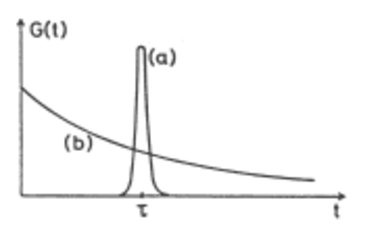
\includegraphics[width=.350\textwidth]{Immagini/exponential.pdf}}
\caption{Two possible choices (curves a and b) for the synaptic delay function G(t).}
\label{fig:exponential}
\end{figure}
For the exponential delay function the interesting range of A is between 1 and 2. The temporal distance between transitions of patterns diverges at the lower boundary $(A = 1)$, and decreases to the value $t_{0} =\tau \log(2)$ at $(A = 2)$. An interesting special case is that of a single pattern a and the synapses
\begin{equation}
    w_{ij}^{S}=-\lambda \sigma_{i}\sigma_{j} \qquad 
    w_{ij}^{S}=\sigma_{i}\sigma_{j}
\end{equation}

which cause the network to oscillate between the pattern and its inverse.
In this manner one can construct neural networks that permanently cycle between states of high and low activity. In addition to the possibility of going through periodic cycles of p patterns or of getting stuck at one of the patterns (if A is too small), a further kind of temporal behavior has been observed for the case of the exponential synaptic delay function $G(t)$ . If the parameter A is chosen sufficiently large then the network switches to chaotic time evolution, tumbling through a set of distorted patterns in a highly irregular fashion.

\subsection{Stochastic neurons}\label{sec:Stochasticneurons}
We now consider a simple generalization of the neural networks discussed in the previous sections which permits a more powerful theoretical treatment.
For this purpose we replace the deterministic evolution law
\begin{equation}\label{DeterministicNetwork}
s_i(t+1)=\sgn{\bigl[h_i(t)\bigr]}=\sgn{\left[\sum_{j=1}^Nw_{ij}s_j(t)\right]}
\end{equation}
for the neural activity by a \emph{stochastic law}, which does not assign a definite value to $s_i(t+1)$, but only gives the probabilities that $s_i(t+1)$ takes one of the values $+1$ or $-1$. In particular we request that
%\begin{equation}
%\operatorname{Pr}\bigl[s_i(t+1)\bigr]=f\bigl[h_i(t)\bigr]
%\end{equation}
\begin{equation}
\operatorname{Pr}\bigl[s_i(t+1)=+1\bigr]=f\bigl[h_i(t)\bigr]
\end{equation}
where the activation function $f(h)$ must have the proper limiting values $f(h\rightarrow-\infty)=0$, $f(h\rightarrow+\infty)=1$. Between these limits the activation function must rise monotonously. A standard choice, depicted in Figure~\ref{f(h)}, is given by
\begin{equation}\label{sigmoidal}
f(h)=\frac{1}{1+e^{-2\beta h}}
\end{equation}
which satisfies the condition
\begin{equation}
f(h)+f(-h)=1
\end{equation}
Accordingly, since $\operatorname{Pr}\bigl[s_i(t+1)=-1\bigr]=1-f\bigl[h_i(t)\bigr]$, we can explicit our stochastic law as
\begin{gather}
\operatorname{Pr}\bigl[s_i(t+1)=+1\bigr]=f\bigl[+h_i(t)\bigr]\\
\operatorname{Pr}\bigl[s_i(t+1)=-1\bigr]=f\bigl[-h_i(t)\bigr]
\end{gather}
that is the values $s_i(t+1)=\pm1$ will occur with probability $f(\pm h_i)$.

The shape of the function $f(h)$ is essentially that of a Fermi--Dirac distribution\footnote{The step is now placed at $h=0$ and unlike the Fermi function it grows monotonously.}\footnote{Such functions are often called \emph{sigmoidal} functions.}, which describes the thermal energy distribution in a system of identical fermions. In that case the parameter $\beta$ has the meaning of an inverse temperature, $\beta=T^{-1}$ (imagine the thermodynamic beta $\beta=1/(k_{\text{B}}T)$ in natural units). We shall also use this nomenclature in connection with neural networks, although this does not imply that the parameter $\beta^{-1}$ should denote a physical temperature at which the network operates. The rule \eqref{sigmoidal} should rather be considered as a model for a stochastically operating network which has been conveniently designed to permit application of the powerful formal methods of statistical physics. In other words, $\beta^{-1}$ is essentially a pseudo-temperature, i.e. an artifical parameter that has been called ``temperature'' in analogy with statistical physics, but that have a completely different meaning. Notice that in the limit $\beta\rightarrow\infty$, or $T\rightarrow0$, the Fermi function \eqref{sigmoidal} approaches the unit step function $\Theta(h)$. This means that at very low temperature the stochastic neural network goes over into our original deterministic network \eqref{DeterministicNetwork}. Hence all results obtained for stochastic networks can be extrapolated to the deterministic case.
\begin{figure}[ht]
\centering
\pgfplotsset{
layers/personal/.define layer set={axis background,axis grid,pre main,main,axis ticks,axis lines,axis tick labels,axis descriptions,axis foreground}{
	grid style				= {/pgfplots/on layer=axis grid},
	tick style				= {/pgfplots/on layer=axis ticks},
	axis line style			= {/pgfplots/on layer=axis lines},
	label style				= {/pgfplots/on layer=axis descriptions},
	legend style			= {/pgfplots/on layer=axis descriptions},
	title style				= {/pgfplots/on layer=axis descriptions},
	colorbar style			= {/pgfplots/on layer=axis descriptions},
	ticklabel style			= {/pgfplots/on layer=axis tick labels},
	axis background@ style		= {/pgfplots/on layer=axis background},
	3d box foreground style	= {/pgfplots/on layer=axis foreground},
},}
\pgfmathsetmacro{\b}{2.6}
\begin{tikzpicture}
\begin{axis}[set layers=personal,width=9cm,height=6.75cm,ylabel={$f(h)$},xlabel={$h$},axis x line=middle,axis y line=middle,x label style={at={(ticklabel* cs:1)},anchor=west},y label style={at={(ticklabel* cs:1)},anchor=south},xmin=-2,xmax=2,ymin=-1.5,ymax=1.8,xtick={-1/\b,1/\b},xticklabels={$-\dfrac{1}{\beta}$,$+\dfrac{1}{\beta}$},ytick={-1,1},yticklabels={$-1$,$+1$}]
\draw[lightgray,dashed] (axis cs:0,1) -- (axis cs:2,1);
\draw[lightgray,dashed] (axis cs:-1/\b,0) -- (axis cs:-1/\b,{1/(1+e^(-2*\b*(-1/\b)))});
\draw[lightgray,dashed] (axis cs:+1/\b,0) -- (axis cs:+1/\b,{1/(1+e^(-2*\b*(+1/\b)))});
\addplot[very thick,smooth,samples=80,domain=-2:2]{1/(1+e^(-2*\b*x))};
\end{axis}
\end{tikzpicture}
\caption{}\label{f(h)}
\end{figure}

The exact state of a given neuron in a stochastic network is not of particular relevance, because it is determined randomly. However, the \emph{mean activity} of a neuron (or the mean orientation of a spin in the magnetic analogy) is an interesting quantity. Let us first consider a single neuron; its mean activity is given by
\begin{equation}
\begin{split}
\langle s\rangle&=(+1)f(h)+(-1)f(-h)\\
&=\frac{1}{1+e^{-2\beta h}}-\frac{1}{1+e^{2\beta h}}\\
&=\frac{1}{1+e^{-2\beta h}}-\frac{e^{-2\beta h}}{1+e^{-2\beta h}}\\
&=\frac{1-e^{-2\beta h}}{1+e^{-2\beta h}}\\
&=\frac{e^{\beta h}-e^{-\beta h}}{e^{\beta h}+e^{-\beta h}}\\
&=\tanh{(\beta h)}
\end{split}
\end{equation}
As already said, in the limit $\beta\rightarrow\infty$ one obtains $\langle s\rangle=\sgn{(h)}$, i.e., depending on the sign of the local field $h$, the neuron is either permanently active or permanently dormant (again, we recover the deterministic result).
\begin{figure}[ht]
\centering
\pgfplotsset{
layers/personal/.define layer set={axis background,axis grid,pre main,main,axis ticks,axis lines,axis tick labels,axis descriptions,axis foreground}{
	grid style				= {/pgfplots/on layer=axis grid},
	tick style				= {/pgfplots/on layer=axis ticks},
	axis line style			= {/pgfplots/on layer=axis lines},
	label style				= {/pgfplots/on layer=axis descriptions},
	legend style			= {/pgfplots/on layer=axis descriptions},
	title style				= {/pgfplots/on layer=axis descriptions},
	colorbar style			= {/pgfplots/on layer=axis descriptions},
	ticklabel style			= {/pgfplots/on layer=axis tick labels},
	axis background@ style		= {/pgfplots/on layer=axis background},
	3d box foreground style	= {/pgfplots/on layer=axis foreground},
},}
\pgfmathsetmacro{\b}{3}
\begin{tikzpicture}
\begin{axis}[set layers=personal,width=9cm,height=6.75cm,ylabel={$\langle s\rangle$},xlabel={$h$},axis x line=middle,axis y line=middle,x label style={at={(ticklabel* cs:1)},anchor=west},y label style={at={(ticklabel* cs:1)},anchor=south},xmin=-2,xmax=2,ymin=-1.65,ymax=1.65,xtick={-1/\b,1/\b},xticklabels={$-\dfrac{1}{\beta}$\hspace*{15pt},$+\dfrac{1}{\beta}$},ytick={1,-1},yticklabels={$+1$,$-1$},y tick label style={outer sep={0.02pt+0.13em},inner sep={0.33333em-0.13em},fill=white,fill opacity=0.75,text opacity=1,xshift={mod(\ticknum,2)*2.385em},/pgfplots/on layer=axis ticks}]
\draw[lightgray,dashed] (axis cs:-2,1) -- (axis cs:2,1);
\draw[lightgray,dashed] (axis cs:-2,-1) -- (axis cs:2,-1);
%\draw[lightgray,dashed] (axis cs:-1/\b,0) -- (axis cs:-1/\b,{1/(1+e^(-2*\b*(-1/\b)))});
%\draw[lightgray,dashed] (axis cs:+1/\b,0) -- (axis cs:+1/\b,{1/(1+e^(-2*\b*(+1/\b)))});
\addplot[very thick,smooth,samples=80,domain=-2:2]{tanh(\b*x)};
\end{axis}
\end{tikzpicture}
\caption{The function $\langle s\rangle=\tanh{(\beta h)}$.}\label{mean(s)}
\end{figure}

The evolution of a single neuron $i$ in a network composed of many elements is difficult to describe, since its state depends on \emph{all} other neurons, which continually fluctuate between $+1$ and $-1$. That even remains true if we are only interested in the mean activity of the $i$-th neuron. This is determined by the value of the synaptic potential $h_i$, which depends, however, on the actual instantaneous states $s_j$ of the other neurons and not on their mean activities. The difficulty is a result of the non-linearity of the probability function $f(h)$, which does not permit one to take the average in the argument of the function. In such cases one often resorts to a technique called the \textbf{mean-field approximation}.

We have already seen the mean-field approximation in many contexts: in solid state physics, statistical physics and nuclear physics also. In those cases we used to study many-body problems (for example systems of interacting fermions) of which we were given the total Lagrangian. By solving the Euler--Lagrange equations, one is able to construct a system of (often coupled) equations which then had to be solved to determine the evolution of the individual fields. The problem arises from the fact that usually we work in a quantum regime, and not in a classical one; so the fields to be determined are actually operators, and not numbers. An operator is a more complicated object because it contains a lot of information, although one usually takes the expectation value to get some measure of probability. Consequently, the interaction terms within the equations of motion become almost unmanageable for many-body problems, as each field depends on the local value of all the other fields. The idea of the mean-field approximation is therefore to systematically reduce quantum fields into classical fields, that is to see them no longer as operators, but as numbers. In practice, instead of quantum fields, their expectation value was substituted: $\widehat{\psi}\rightarrow\langle\widehat{\psi}\rangle$. In this way the many-body problem is simplified in a one-body problem, because the total intricate interaction is replaced with a \emph{mean field} generated by all the others (i.e. no more many-body-dependent). In other words, this technique allows us to factor out the terms of interactions and to obtain, by adding them, a single interaction field that describes the average potential generated by all the particles together. The mean-field approximation becomes particularly useful when we have to deal simultaneously with many bodies (indeed, it is sometimes called large-$N$ approximation).

Returning to our neural networks, here we basically want to do the same thing, and therefore we can define the mean-field approximation as the exchange operation between the synaptic potential with its average value
\begin{equation}
f(h_i)\xrightarrow{\text{MFA}}f\bigl(\langle h_i\rangle\bigr)=f\!\left(\sum_{j=1}^Nw_{ij}\langle s_j\rangle\right)
\end{equation}
The mean activity of a neuron is then computable as before:
\begin{equation}
\langle s_i\rangle=(+1)f\bigl(\langle h_i\rangle\bigr)+(-1)f\bigl(-\langle h_i\rangle\bigr)
\end{equation}
whence
\begin{equation}\label{StochasticNetwork}
\boxed{\langle s_i\rangle=\tanh{\left(\beta\sum_{j=1}^Nw_{ij}\langle s_j\rangle\right)}}
\end{equation}
This is still a system of nonlinear equations with $N$ unknowns $\langle s_i\rangle$, but these have become deterministic rather than stochastic variables.
\subsubsection{Single pattern}
The solution of the system of equations \eqref{StochasticNetwork} depends, of course, on the choice of the synaptic strengths $w_{ij}$. We begin by considering the simplest case of a single pattern
\begin{equation}
w_{ij}=\frac{1}{N}\sigma_i\sigma_j
\end{equation}
Assuming also that all bits are equal ($+1$ or $-1$, it doesn't matter) we can further simplify it as $w_{ij}=1/N$ for all $i, j$. One could be skeptical about this assumption, but it is essentially a gauge transformation, since it corresponds to a reinterpretation of the meaning of ``up'' and ``down'' at each lattice site.

Anyway, in this case equation \eqref{StochasticNetwork} becomes
\begin{equation}
\langle s_i\rangle=\tanh{\left(\beta\frac{1}{N}\sum_{j=1}^N\langle s_j\rangle\right)}\qquad\text{for all $i$}
\end{equation}
and because the right-hand side does not depend on $i$ we can write
\begin{equation}\label{TranscendentalEquation}
\langle s\rangle=\tanh{\bigl(\beta\langle s\rangle\bigr)}
\end{equation}
(of course $\langle s_i\rangle=\langle s_j\rangle$ since we don't have any reason to suppose they are different). We have thus managed to reduce the evolution law to a single equation, but is still a transcendental equation; therefore we must solve it graphically, i.e. we have to find graphically the possible intersections between the straight line $\langle s\rangle$ and the hyperbolic tangent $\tanh{\bigl(\beta\langle s\rangle\bigr)}$. Recall that the hyperbolic tangent is monotonously increasing and from 0 to $\infty$ its slope always diminishes (vice versa, from $-\infty$ to $0$ it systemically increases, due to symmetry reason). Based on this observation, we deduce that we have to compare the behavior of the two functions at the origin, where the slope has its maximum value. In particular, we have to distinguish two cases illustrated in Figure~\ref{Intersections}. For $\beta<1$ ($T>1$) equation \eqref{TranscendentalEquation} admits only the trivial solution at $\langle s\rangle=0$ because the slope of the line is higher than that of the hyperbolic tangent (Fig.~\ref{1Solution}). So at large temperature the bits continuously flip between $+1$ and $-1$, but with null expectation value, meaning that the network is essentially unable to memorize any information. Instead, for $\beta>1$ ($T<1$) equation \eqref{TranscendentalEquation} admits altogether three solutions, namely $\langle s\rangle=-\overline{s},0,\overline{s}$ because the slope of the line is smaller than that of the hyperbolic tangent (Fig.~\ref{3Solutions}). However, it is possible to show that $\langle s\rangle=\pm\overline{s}$ correspond to a stable minimum configurations of the system, while $\langle s\rangle=0$ corresponds to a local maximum, which is unstable! In fact, the hyperbolic tangent is very stiff close to 0; hence any small perturbation from $\langle s\rangle=0$ makes the system change rapidly either towards $-1$ or $+1$. Therefore, we neglect this possibility at low temperature. Finally, the limiting situation is that in which the straight line is exactly tangent to the hyperbolic tangent, corresponding to $\beta=T=1$ (which takes the role of critical, or Curie, temperature separating the two different regimes). This analytical behavior at $T=1$ is indeed very similar to a \emph{phase transition} in which at high temperature the system is chaotic, whereas at low temperature it presents an oriented structure (like ferromagnetism).
\begin{figure}[ht]
\centering
\pgfplotsset{
	layers/personal/.define layer set={axis background,axis grid,axis ticks,axis lines,axis tick labels,axis descriptions,pre main,main,axis foreground}{
		grid style				= {/pgfplots/on layer=axis grid},
		tick style				= {/pgfplots/on layer=axis ticks},
		axis line style			= {/pgfplots/on layer=axis lines},
		label style				= {/pgfplots/on layer=axis descriptions},
		legend style			= {/pgfplots/on layer=axis descriptions},
		title style				= {/pgfplots/on layer=axis descriptions},
		colorbar style			= {/pgfplots/on layer=axis descriptions},
		ticklabel style			= {/pgfplots/on layer=axis tick labels},
		axis background@ style		= {/pgfplots/on layer=axis background},
		3d box foreground style	= {/pgfplots/on layer=axis foreground},
	},}
\begin{subfigure}[ht]{0.49\textwidth}
	\centering
        \pgfmathsetmacro{\b}{0.95}
	\begin{tikzpicture}
	\begin{axis}[set layers=personal,width=8cm,height=6.75cm,ylabel={$g\bigl(\langle s\rangle\bigr)$},xlabel={$\langle s\rangle$},axis x line=middle,axis y line=middle,x label style={at={(ticklabel* cs:1)},anchor=west},y label style={at={(ticklabel* cs:1)},anchor=south},xmin=-2,xmax=2,ymin=-1.65,ymax=1.65,xtick=\empty,ytick={1,-1},yticklabels={$+1$,$-1$},y tick label style={outer sep={0.02pt+0.13em},inner sep={0.33333em-0.13em},fill=white,fill opacity=0.75,text opacity=1,xshift={mod(\ticknum,2)*2.385em},/pgfplots/on layer=main}]
	\addplot[lightgray,dashed,samples=2,domain=-2:2,on layer=axis grid] {1};
	\addplot[lightgray,dashed,samples=2,domain=-2:2,on layer=axis grid] {-1};
	\addplot[very thick,smooth,samples=80,domain=-2:2]{tanh(\b*x)};
	\addplot[very thick,blue,samples=2,domain=-2:2]{x};
	\addplot[only marks,mark=*,mark size=3pt,mark options={fill=white}] coordinates {(0,0)};
	\end{axis}
	\end{tikzpicture}
        \caption{$\beta<1$: only one solution.}\label{1Solution}
\end{subfigure}
\hfill
\begin{subfigure}[ht]{0.49\textwidth}
	\centering
	\pgfmathsetmacro{\b}{3}
	\begin{tikzpicture}
	\begin{axis}[set layers=personal,width=8cm,height=6.75cm,ylabel={$g\bigl(\langle s\rangle\bigr)$},xlabel={$\langle s\rangle$},axis x line=middle,axis y line=middle,x label style={at={(ticklabel* cs:1)},anchor=west},y label style={at={(ticklabel* cs:1)},anchor=south},xmin=-2,xmax=2,ymin=-1.65,ymax=1.65,xtick={0.9994902,-0.9994902},xticklabels={$\overline{s}$,$\overline{s}$},ytick={1,-1},yticklabels={$+1$,$-1$},x tick label style={outer sep={0.02pt+0.13em},inner sep={0.33333em-0.13em},fill=white,fill opacity=0.75,text opacity=1,yshift={mod(\ticknum,2)*1.585em},/pgfplots/on layer=main},y tick label style={outer sep={0.02pt+0.13em},inner sep={0.33333em-0.13em},fill=white,fill opacity=0.75,text opacity=1,xshift={mod(\ticknum,2)*2.385em},/pgfplots/on layer=main}]
	\addplot[lightgray,dashed,samples=2,domain=-2:2,on layer=axis grid] {1};
	\addplot[lightgray,dashed,samples=2,domain=-2:2,on layer=axis grid] {-1};
	\addplot[lightgray,dashed,on layer=axis grid] coordinates {(-0.9994902,0) (-0.9994902,-0.9994902)};
	\addplot[lightgray,dashed,on layer=axis grid] coordinates {(0.9994902,0) (0.9994902,0.9994902)};
	\addplot[very thick,smooth,samples=80,domain=-2:2]{tanh(\b*x)};
	\addplot[very thick,blue,samples=2,domain=-2:2]{x};
	\addplot[only marks,mark=*,mark size=3pt,mark options={fill=white}] coordinates {(-0.9994902,-0.9994902) (0,0) (0.9994902,0.9994902)};
	\end{axis}
	\end{tikzpicture}
        \caption{$\beta>1$: three solutions.}\label{3Solutions}
\end{subfigure}
\caption{Intersections between $\langle s\rangle$ and $\tanh{\bigl(\beta\langle s\rangle\bigr)}$.}\label{Intersections}
\end{figure}
\subsubsection{Several patterns}
We now turn to the general situation, when the synaptic couplings are fixed according to Hebb's rule
\begin{equation}
w_{ij}=\frac{1}{N}\sum_{\mu=1}^p\sigma_i^\mu\sigma_j^\mu
\end{equation}
for several patterns. The mean-field equation \eqref{StochasticNetwork} then takes the form
\begin{equation}\label{Several patternsEq}
\langle s_i\rangle=\tanh{\left(\frac{\beta}{N}\sum_{j=1}^N\sum_{\mu=1}^p\sigma_i^\mu\sigma_j^\mu\langle s_j\rangle\right)}
\end{equation}
This relation does not have an obvious solution. However, we recall that every single stored pattern represents a stable configuration for a deterministic network. It is, therefore, not unreasonable to make the \emph{ansatz}\footnote{An ansatz (from German) is an educated guess or an additional assumption made to help solve a problem, and which is later verified to be part of the solution by its results.} that $\langle s_i\rangle$ resembles one of the stored patterns, except for a normalization factor:
\begin{equation}
\langle s_i\rangle=m\sigma_i^\nu
\end{equation}
Inserting this into \eqref{Several patternsEq} and assuming as usual that the memorized patterns are completely uncorrelated we obtain
\begin{equation}
\begin{split}
m\sigma_i^\nu&=\tanh{\left(\frac{\beta m}{N}\sum_{j=1}^N\sum_{\mu=1}^p\sigma_i^\mu\sigma_j^\mu\sigma_j^\nu\right)}\\
&=\tanh{\left(\frac{\beta m}{N}\sum_{j=1}^N\sigma_i^\nu\overbrace{\sigma_j^\nu\sigma_j^\nu}^{=1}+\frac{\beta m}{N}\sum_{\mu\neq\nu}\sigma_i^\mu\sum_{j=1}^N\sigma_j^\mu\sigma_j^\nu\right)}\\
&=\tanh{\left[\beta m\sigma_i^\nu+\beta m\mathcal{O}\Biggl(\sqrt{\frac{p-1}{N}}\Biggr)\right]}
\end{split}
\end{equation}
As long as $p\ll N$ the second term is clearly negligible:
\begin{equation}
m\sigma_i^\nu\simeq\tanh{(\beta m\sigma_i^\nu)}
\end{equation}
Moreover, on account of $\sigma_i^\nu=\pm1$, i.e. $\tanh{(-x)}=-\tanh{x}$ (it is an odd function), the normalization factor $m$ (and consequently $\langle s_i\rangle$) is determined by the same equation
\begin{equation}
m=\tanh{(\beta m)}
\end{equation}
Again we find the same fixed points as for a single stored pattern: for $T>1$ one has $m=0$, and the time-averaged network configuration does not resemble one of the stored patterns. One might say that the network is ``amnesic''. For $T<1$ one has $m=\pm\overline{s}$ and the average configuration of the network points toward one of the stored patterns. Since these take only the values $\pm1$, the patterns can be uniquely (up to an overall sign) recovered from the averaged state $\langle s_i\rangle$ of the network.

Numerical simulations as well as statistical analysis show that the number of stored patterns relative to the number of neurons, $\alpha=p/N$, plays a similar role as the parameter $T$. When the storage utilization $\alpha$ is increased starting from zero, i.e. if more and more patterns are stored, the recall quality of the network deteriorates slightly. However, when $\alpha$ approaches the critical capacity $\alpha_c\approx0.138$, the network suddenly and catastrophically fails to recall any of the memorized patterns. In other words the networks suddenly jumps from almost perfect memory into a state of complete confusion.

In order to obtain a complete description of the ability of a stochastic Hopfield network to recall memorized patterns one has to consider $m$ as function of $\alpha$ as well as of $T$. One then obtains a complete phase diagram of
the \emph{order parameter} $m(T,\alpha)$. The phase boundary between ``functioning memory'' and total ``confusion'' or ``amnesia'' is given by a line in the $\alpha$--$T$ diagram, depicted in Figure~\ref{OrderParameter}. For $T=0$ this line begins at $\alpha_c\approx0.138$ and ends, as we just have found, at $T=1$ for $\alpha=0$. At the phase boundary $m$ falls discontinuously to zero, except for $T= 0$, where the change is continuous, but not differentiable\footnote{Note that these results strictly apply only in the thermodynamic limit $N\rightarrow\infty$, i.e. for systems with infinitely many neurons.}.
\begin{figure}[h!t]
\centering
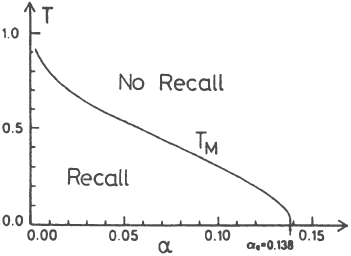
\includegraphics[scale=0.85]{Order Parameter}
\caption{Memory recall is possible only in a finite region of temperatures $T$ and storage density $\alpha=p/N$.}\label{OrderParameter}
\end{figure}

In addition to its usefulness in the formal treatment of neural-network properties the introduction of a stochastic neuron evolution law has important practical advantages. The thermal fluctuations reduce the probability that the network becomes caught in a spurious, undesired locally stable configuration.
\subsection{Special Learning Rules}\label{sec:Speciallearningrules}
As we discussed in previous sections, the standard learning rule (Hebb's rule) leads to the emergence of undesirable local minima in the ``energy'' functional $E[s]$. In practice, this means that the evolution of the network can be caught in spurious, locally stable configurations. Large networks usually contain a vast number of such spuriously stable states, many of which are not even linear combinations of the desired stability points. Even the learning rule for correlated patterns discussed in Section~\ref{Sec:DOm} does not guard against this problem. Thermal fluctuations do help to destabilize the spurious configurations, but at the expense of storage capacity. Moreover, the disappearance of all the spurious states at some finite $T$ is not ensured.

A much better strategy is to eliminate the undesired stable configurations by appropriate modifications of the synaptic connections. Hopfield et al. have proposed to make use of the fact that the spurious minima of the energy functional $E[s]$ are usually much shallower than the minima that correspond to the learned patterns. Borrowing ideas developed in the study of human dream sleep\footnote{The sleep is commonly divided in two phases, referred to as REM (rapid eye movement) and non-REMs, which is a collection of other stages. The REM phase is characterized by random rapid movement of the eyes, accompanied by low muscle tone throughout the body, and the propensity of the sleeper to dream vividly. Modern studies believe that the purpose of dream sleep (REM sleep) is the elimination of undesirable states of memory.}, they suggested tracking these states by starting the network in some randomly chosen initial configuration and running it until it ends up in a stable equilibrium state $s_i^\infty$. This may be one of the regular learned patterns, or one of the many spurious states. Then, we build new synaptic connections according to the new Hebb's rule:
\begin{equation}\label{REM}
w_{ij}\rightarrow w_{ij}-\frac{\lambda}{N}s_i^\infty s_j^\infty
\end{equation}
where $\lambda\ll1$ is chosen (indeed we are weakening connections), and we let the network run again, until it reaches another equilibrium state $s_i^\infty$. After we build another $w_{ij}$ and we let evolve, and so on and so forth. This iterative procedure must be repeated a large number of times, until we actually fall in one of the global minima. Note that whatever the resulting state is in each iteration, through \eqref{REM} the synapses are partially weakened at each step. This procedure of unlearning has two favorable effects. Most spurious equilibrium states of the network are ``forgotten'', since they are already destabilized by small changes in the synaptic connections $w_{ij}$. Moreover, the different regions of stability of the stored patterns become more homogeneous in size, since those with a larger range of stability occur more often as final configurations and are therefore weakened more than others.

The effect of this intentional forgetting is especially apparent in the sizes of the ``basins of attraction''. This term denotes the set of all states, from which the network dynamics leads to a particular pattern (e.g. $\sigma^\mu$). The change of the size of the basin of attraction of a given stored pattern, as the total memory load $\alpha=p/N$ is increased, is illustrated in Figure~\ref{BasinofAttraction}. The two axes labeled $H_k$ and $H_{N-k}$ in these figures represent a crude measure of the distance of an initial trial state $s_i$ from the considered memory state $\sigma_i^\mu$. They denote the partial Hamming distances between the trial state and the memory state, evaluated for the first $k$ and the last $N-k$ of all $N=200$ neurons (for instance), respectively:
\begin{gather}
H_{k}=\frac{1}{4}\sum_{i=1}^{k}{\bigl(s_i-\sigma_i^\mu\bigr)}^2\\
H_{N-k}=\frac{1}{4}\sum_{i=k}^{N-k}{\bigl(s_i-\sigma_i^\mu\bigr)}^2
\end{gather}
In this specific case $k=N/2$ was taken, i.e. the axes represent the Hamming distance for the first and the last half of the neurons of the network. If the trial state $s_i$ developed into the stored pattern $\sigma_i^\mu$, a black dot was plotted.

For a single memory state (Fig.~\hyperref[BasinofAttraction]{\ref*{BasinofAttraction}a}), half of the trial states are found to evolve into the stored pattern $\sigma_i$, while the other half ends up in the complementary pattern $-\sigma_i$. The basin of attraction thus represents a black triangle. This is essentially the result that we have discussed in Section~\ref{LHR}: if we have only one pattern, a random configuration of the network with some altered bits converges to the stored pattern if the number of wrong bits $n$ is smaller than $N/2$. And indeed, any set of $s_i$ (i.e. any different trial configuration) which produces a couple $(H_k,H_{N-k})$ inside the black triangle satisfies this constraint, thus converging to the stored pattern $\sigma_i$. On the other hand, if those trial states are outside the triangle, meaning they are nearer to the complementary pattern $-\sigma_i$ than $\sigma_i$, then the net will converge to $-\sigma_i$ (which is not what we want). Just to make things clearer, if we take a trial state giving $(H_k,H_{N-k})=(100,0)$, then the network configuration will develop into the memorized pattern because it means that half of the initial bits are exact ($H_{N-k}=0$), while the other half are wrong ($H_{k}=100$).

What now happens if we increase the number of stored patterns? For more memory states the basin of attraction shrinks rapidly and takes on a highly ragged shape in the vicinity of $\alpha_c\approx0.138$, as shown in Figures~\hyperref[BasinofAttraction]{\ref*{BasinofAttraction}b,\,c} for 28 and 32 uncorrelated memory states, respectively. In fact, when we are above the critical storage threshold $\alpha_c$ the network becomes no more able to retrieve memorized patterns.

Finally Figure~\hyperref[BasinofAttraction]{\ref*{BasinofAttraction}d} shows the result of applying the forgetting algorithm \eqref{REM} 1000 times to the network loaded with 32 patterns and $\lambda=0.01$. The basin of attraction grows strongly (by a factor of ten or more) and also takes on a more regular shape. The probability of retrieving the stored patterns is much improved (so ``forgetting improves the memory'').
\begin{figure}[h!t]
\centering
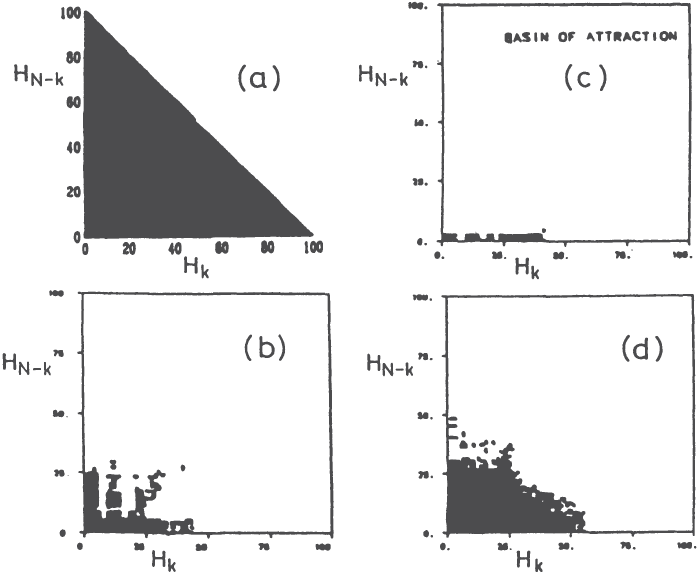
\includegraphics[scale=0.75]{Basin of Attraction}\hspace{7pt}
\caption{Basins of attraction in a Hopfield network with 200 neurons for (a) 1, (b) 28, (c) 32 memory states. After deliberate forgetting the basin expands strongly (d).}\label{BasinofAttraction}
\end{figure}

{\small
In a somewhat modified version of this method the network is allowed to develop from the stored patterns, deteriorated by random noise. One then not only weakens the synaptic connections by unlearning the final state $s_i^\infty$, but also simultaneously relearns the correct starting pattern $\nu$:
\begin{equation}\label{REMmodified}
w_{ij}\rightarrow w_{ij}-\frac{\lambda}{N}\Bigl(s_i^\infty s_j^\infty-\sigma_i^\nu\sigma_j^\nu\Bigr)
\end{equation}
If the pattern was recalled without fault, the synapses remain unchanged according to this prescription. With this method the storage capacity can be increased to $\alpha=1$, and the storage of strongly correlated patterns becomes possible.\par}

\section{Perceptrons}
\subsection{Simple perceptron}\label{Sec:SimplePerceptron}
The neural network models discussed so far were all aimed at storing and recalling given information. Memory is an important function of the brain, but far from the only one. Another important task of the central nervous system is to learn reactions and useful behavior that permit survival in an often hostile environment. In a highly simplified perspective one may identify this role of the brain with that of the supervising element in a control circuit. We shall therefore introduce the term \emph{cybernetic networks} for neural networks that provide an optimal reaction or answer to an external stimulus. Such networks usually have a structure that fundamentally differs from that of memory networks. In particular, the synaptic connections are generally not symmetric ($w_{ij}\neq w_{ji}$); often they are maximally asymmetric, i.e. unidirectional. As a result, the theories of thermodynamic equilibrium systems have no direct application to cybernetic networks, and much less general insights are known into their behavior.
%\begin{equation}
%w_{ij}=\frac{1}{N}\sum_{\mu=1}^p\sigma_i^\mu\sigma_j^\mu=w_{ji}
%\end{equation}

The best-studied class of cybernetic networks are the so-called \emph{feed-forward layered} neural networks, or simply \textbf{perceptrons}, where information flows in one direction between several distinct layers of neurons, as illustrated in Figure~\ref{Perceptron}. At one end is the \emph{input} layer composed of sensory neurons, which receive external stimuli, at the other end is an \emph{output} layer often composed of motor neurons, which cause the desired reaction.
\begin{figure}[h!t]
\centering
\pgfmathsetmacro{\h}{1.5}
\pgfmathsetmacro{\x}{1.0}
\begin{tikzpicture}[line width=0.2pt]
\draw[lightgray!30,line width=1mm,line cap=round] (-0.6,0) -- (6.6,0);
%\draw[lightgray!30,line width=1mm,line cap=round] (-0.6,-1.2) -- (6.6,-1.2);
%\draw[lightgray!30,line width=1mm,line cap=round] (-0.6,-2.4) -- (6.6,-2.4);
\draw[lightgray!30,line width=1mm,line cap=round] (-0.6,-3*\h) -- (6.6,-3*\h);
\fill[top color=lightgray!30,bottom color=lightgray!30,middle color=lightgray!5,line join=round] (-0.65,-2*\h-0.05) rectangle (6.65,-1*\h+0.05);
%\foreach \i in {0,...,3,4.5} {
%	\fill[ball color=white] (\i+0.5,-4/3*\h) circle (0.2);
%	\fill[white,opacity=0.9] (\i+0.5,-4/3*\h) circle (0.2);
%}
%\foreach \i in {0,...,3,4.5} {
%	\fill[ball color=white] (\i+0.5,-5/3*\h) circle (0.2);
%	\fill[white,opacity=0.9] (\i+0.5,-5/3*\h) circle (0.2);
%}
\foreach \i in {0,...,3,4.5} {
	\fill[ball color=white] (\i+0.5,-1.5*\h) circle (0.2);
	\fill[white,opacity=0.9] (\i+0.5,-1.5*\h) circle (0.2);
}
%Stimuli, Reaction
\foreach \i in {0,...,4,5.5} {\draw[-stealth,very thick] (\i*\x,1.1) -- (\i*\x,0.3);}
\draw[decorate,decoration={brace,amplitude=5pt},thick] (-0.2,1.2) -- (5.7,1.2) node[midway,anchor=south,inner sep=0pt,yshift=0.3cm]{External stimuli};
\foreach \i in {1,...,3,4.5} {\draw[-stealth,very thick] (\i*\x,-3*\h) -- (\i*\x,-3*\h-1.05);}
\draw[decorate,decoration={brace,mirror,amplitude=5pt},thick] (0.8,-3*\h-1.15) -- (4.7,-3*\h-1.15) node[midway,anchor=north,inner sep=0pt,yshift=-0.3cm]{Reaction};
%Input->Hidden
\draw[-stealth] (0,0) --+ ({-atan(\h/0.5)}:{sqrt((\h)^2+(0.5*\x)^2)-0.25});
\draw[-stealth] (0,0) --+ ({-atan(\h/1.5)}:{sqrt((\h)^2+(1.5*\x)^2)-0.25});
\draw[-stealth] (0,0) --+ ({-atan(\h/2.5)}:{sqrt((\h)^2+(2.5*\x)^2)-0.25});
\draw[-stealth] (0,0) --+ ({-atan(\h/3.5)}:{sqrt((\h)^2+(3.5*\x)^2)-0.25});
\draw[-stealth] (0,0) --+ ({-atan(\h/5.0)}:{sqrt((\h)^2+(5.0*\x)^2)-0.25});
\draw[-stealth] (\x,0) --+ ({180+atan(\h/0.5)}:{sqrt((\h)^2+(0.5*\x)^2)-0.25});
\draw[-stealth] (\x,0) --+ ({-atan(\h/0.5)}:{sqrt((\h)^2+(0.5*\x)^2)-0.25});
\draw[-stealth] (\x,0) --+ ({-atan(\h/1.5)}:{sqrt((\h)^2+(1.5*\x)^2)-0.25});
\draw[-stealth] (\x,0) --+ ({-atan(\h/2.5)}:{sqrt((\h)^2+(2.5*\x)^2)-0.25});
\draw[-stealth] (\x,0) --+ ({-atan(\h/4.0)}:{sqrt((\h)^2+(4.0*\x)^2)-0.25});
\draw[-stealth] (2*\x,0) --+ ({180+atan(\h/1.5)}:{sqrt((\h)^2+(1.5*\x)^2)-0.25});
\draw[-stealth] (2*\x,0) --+ ({180+atan(\h/0.5)}:{sqrt((\h)^2+(0.5*\x)^2)-0.25});
\draw[-stealth] (2*\x,0) --+ ({-atan(\h/0.5)}:{sqrt((\h)^2+(0.5*\x)^2)-0.25});
\draw[-stealth] (2*\x,0) --+ ({-atan(\h/1.5)}:{sqrt((\h)^2+(1.5*\x)^2)-0.25});
\draw[-stealth] (2*\x,0) --+ ({-atan(\h/3.0)}:{sqrt((\h)^2+(3.0*\x)^2)-0.25});
\draw[-stealth] (3*\x,0) --+ ({180+atan(\h/2.5)}:{sqrt((\h)^2+(2.5*\x)^2)-0.25});
\draw[-stealth] (3*\x,0) --+ ({180+atan(\h/1.5)}:{sqrt((\h)^2+(1.5*\x)^2)-0.25});
\draw[-stealth] (3*\x,0) --+ ({180+atan(\h/0.5)}:{sqrt((\h)^2+(0.5*\x)^2)-0.25});
\draw[-stealth] (3*\x,0) --+ ({-atan(\h/0.5)}:{sqrt((\h)^2+(0.5*\x)^2)-0.25});
\draw[-stealth] (3*\x,0) --+ ({-atan(\h/2.0)}:{sqrt((\h)^2+(2.0*\x)^2)-0.25});
\draw[-stealth] (4*\x,0) --+ ({180+atan(\h/3.5)}:{sqrt((\h)^2+(3.5*\x)^2)-0.25});
\draw[-stealth] (4*\x,0) --+ ({180+atan(\h/2.5)}:{sqrt((\h)^2+(2.5*\x)^2)-0.25});
\draw[-stealth] (4*\x,0) --+ ({180+atan(\h/1.5)}:{sqrt((\h)^2+(1.5*\x)^2)-0.25});
\draw[-stealth] (4*\x,0) --+ ({180+atan(\h/0.5)}:{sqrt((\h)^2+(0.5*\x)^2)-0.25});
\draw[-stealth] (4*\x,0) --+ ({-atan(\h/1.0)}:{sqrt((\h)^2+(1.0*\x)^2)-0.25});
\draw[-stealth] (5.5*\x,0) --+ ({180+atan(\h/5.0)}:{sqrt((\h)^2+(5.0*\x)^2)-0.25});
\draw[-stealth] (5.5*\x,0) --+ ({180+atan(\h/4.0)}:{sqrt((\h)^2+(4.0*\x)^2)-0.25});
\draw[-stealth] (5.5*\x,0) --+ ({180+atan(\h/3.0)}:{sqrt((\h)^2+(3.0*\x)^2)-0.25});
\draw[-stealth] (5.5*\x,0) --+ ({180+atan(\h/2.0)}:{sqrt((\h)^2+(2.0*\x)^2)-0.25});
\draw[-stealth] (5.5*\x,0) --+ ({180+atan(\h/0.5)}:{sqrt((\h)^2+(0.5*\x)^2)-0.25});
%Hidden->Hidden
\draw[-stealth,dashed,gray!60] (0.5*\x,-1*\h) --+ (-90:{\h-0.25});
\draw[-stealth,dashed,gray!60] (0.5*\x,-1*\h) --+ ({-atan(\h/1.0)}:{sqrt((\h)^2+(1.0*\x)^2)-0.25});
\draw[-stealth,dashed,gray!60] (0.5*\x,-1*\h) --+ ({-atan(\h/2.0)}:{sqrt((\h)^2+(2.0*\x)^2)-0.25});
\draw[-stealth,dashed,gray!60] (0.5*\x,-1*\h) --+ ({-atan(\h/3.0)}:{sqrt((\h)^2+(3.0*\x)^2)-0.25});
\draw[-stealth,dashed,gray!60] (0.5*\x,-1*\h) --+ ({-atan(\h/4.5)}:{sqrt((\h)^2+(4.5*\x)^2)-0.25});
\draw[-stealth,dashed,gray!60] (1.5*\x,-1*\h) --+ ({180+atan(\h/1.0)}:{sqrt((\h)^2+(1.0*\x)^2)-0.25});
\draw[-stealth,dashed,gray!60] (1.5*\x,-1*\h) --+ (-90:{\h-0.25});
\draw[-stealth,dashed,gray!60] (1.5*\x,-1*\h) --+ ({-atan(\h/1.0)}:{sqrt((\h)^2+(1.0*\x)^2)-0.25});
\draw[-stealth,dashed,gray!60] (1.5*\x,-1*\h) --+ ({-atan(\h/2.0)}:{sqrt((\h)^2+(2.0*\x)^2)-0.25});
\draw[-stealth,dashed,gray!60] (1.5*\x,-1*\h) --+ ({-atan(\h/3.5)}:{sqrt((\h)^2+(3.5*\x)^2)-0.25});
\draw[-stealth,dashed,gray!60] (2.5*\x,-1*\h) --+ ({180+atan(\h/2.0)}:{sqrt((\h)^2+(2.0*\x)^2)-0.25});
\draw[-stealth,dashed,gray!60] (2.5*\x,-1*\h) --+ ({180+atan(\h/1.0)}:{sqrt((\h)^2+(1.0*\x)^2)-0.25});
\draw[-stealth,dashed,gray!60] (2.5*\x,-1*\h) --+ (-90:{\h-0.25});
\draw[-stealth,dashed,gray!60] (2.5*\x,-1*\h) --+ ({-atan(\h/1.0)}:{sqrt((\h)^2+(1.0*\x)^2)-0.25});
\draw[-stealth,dashed,gray!60] (2.5*\x,-1*\h) --+ ({-atan(\h/2.5)}:{sqrt((\h)^2+(2.5*\x)^2)-0.25});
\draw[-stealth,dashed,gray!60] (3.5*\x,-1*\h) --+ ({180+atan(\h/3.0)}:{sqrt((\h)^2+(3.0*\x)^2)-0.25});
\draw[-stealth,dashed,gray!60] (3.5*\x,-1*\h) --+ ({180+atan(\h/2.0)}:{sqrt((\h)^2+(2.0*\x)^2)-0.25});
\draw[-stealth,dashed,gray!60] (3.5*\x,-1*\h) --+ ({180+atan(\h/1.0)}:{sqrt((\h)^2+(1.0*\x)^2)-0.25});
\draw[-stealth,dashed,gray!60] (3.5*\x,-1*\h) --+ (-90:{\h-0.25});
\draw[-stealth,dashed,gray!60] (3.5*\x,-1*\h) --+ ({-atan(\h/1.5)}:{sqrt((\h)^2+(1.5*\x)^2)-0.25});
\draw[-stealth,dashed,gray!60] (5.0*\x,-1*\h) --+ ({180+atan(\h/4.5)}:{sqrt((\h)^2+(4.5*\x)^2)-0.25});
\draw[-stealth,dashed,gray!60] (5.0*\x,-1*\h) --+ ({180+atan(\h/3.5)}:{sqrt((\h)^2+(3.5*\x)^2)-0.25});
\draw[-stealth,dashed,gray!60] (5.0*\x,-1*\h) --+ ({180+atan(\h/2.5)}:{sqrt((\h)^2+(2.5*\x)^2)-0.25});
\draw[-stealth,dashed,gray!60] (5.0*\x,-1*\h) --+ ({180+atan(\h/1.5)}:{sqrt((\h)^2+(1.5*\x)^2)-0.25});
\draw[-stealth,dashed,gray!60] (5.0*\x,-1*\h) --+ (-90:{\h-0.25});
%Hidden->Output
\draw[-stealth] (0.5*\x,-2*\h) --+ ({-atan(\h/0.5)}:{sqrt((\h)^2+(0.5*\x)^2)-0.25});
\draw[-stealth] (0.5*\x,-2*\h) --+ ({-atan(\h/1.5)}:{sqrt((\h)^2+(1.5*\x)^2)-0.25});
\draw[-stealth] (0.5*\x,-2*\h) --+ ({-atan(\h/2.5)}:{sqrt((\h)^2+(2.5*\x)^2)-0.25});
\draw[-stealth] (0.5*\x,-2*\h) --+ ({-atan(\h/4.0)}:{sqrt((\h)^2+(4.0*\x)^2)-0.25});
\draw[-stealth] (1.5*\x,-2*\h) --+ ({180+atan(\h/0.5)}:{sqrt((\h)^2+(0.5*\x)^2)-0.25});
\draw[-stealth] (1.5*\x,-2*\h) --+ ({-atan(\h/0.5)}:{sqrt((\h)^2+(0.5*\x)^2)-0.25});
\draw[-stealth] (1.5*\x,-2*\h) --+ ({-atan(\h/1.5)}:{sqrt((\h)^2+(1.5*\x)^2)-0.25});
\draw[-stealth] (1.5*\x,-2*\h) --+ ({-atan(\h/3.0)}:{sqrt((\h)^2+(3.0*\x)^2)-0.25});
\draw[-stealth] (2.5*\x,-2*\h) --+ ({180+atan(\h/1.5)}:{sqrt((\h)^2+(1.5*\x)^2)-0.25});
\draw[-stealth] (2.5*\x,-2*\h) --+ ({180+atan(\h/0.5)}:{sqrt((\h)^2+(0.5*\x)^2)-0.25});
\draw[-stealth] (2.5*\x,-2*\h) --+ ({-atan(\h/0.5)}:{sqrt((\h)^2+(0.5*\x)^2)-0.25});
\draw[-stealth] (2.5*\x,-2*\h) --+ ({-atan(\h/2.0)}:{sqrt((\h)^2+(2.0*\x)^2)-0.25});
\draw[-stealth] (3.5*\x,-2*\h) --+ ({180+atan(\h/2.5)}:{sqrt((\h)^2+(2.5*\x)^2)-0.25});
\draw[-stealth] (3.5*\x,-2*\h) --+ ({180+atan(\h/1.5)}:{sqrt((\h)^2+(1.5*\x)^2)-0.25});
\draw[-stealth] (3.5*\x,-2*\h) --+ ({180+atan(\h/0.5)}:{sqrt((\h)^2+(0.5*\x)^2)-0.25});
\draw[-stealth] (3.5*\x,-2*\h) --+ ({-atan(\h/1.0)}:{sqrt((\h)^2+(1.0*\x)^2)-0.25});
\draw[-stealth] (5.0*\x,-2*\h) --+ ({180+atan(\h/4.0)}:{sqrt((\h)^2+(4.0*\x)^2)-0.25});
\draw[-stealth] (5.0*\x,-2*\h) --+ ({180+atan(\h/3.0)}:{sqrt((\h)^2+(3.0*\x)^2)-0.25});
\draw[-stealth] (5.0*\x,-2*\h) --+ ({180+atan(\h/2.0)}:{sqrt((\h)^2+(2.0*\x)^2)-0.25});
\draw[-stealth] (5.0*\x,-2*\h) --+ ({180+atan(\h/0.5)}:{sqrt((\h)^2+(0.5*\x)^2)-0.25});
%Neurons
\foreach \i in {0,...,4,5.5} {\fill[ball color=white] (\i,0) circle (0.2);}
\foreach \i in {0,...,3,4.5} {\fill[ball color=white] (\i+0.5,-1*\h) circle (0.2);}
\foreach \i in {0,...,3,4.5} {\fill[ball color=white] (\i+0.5,-2*\h) circle (0.2);}
\foreach \i in {0,...,2,3.5} {\fill[ball color=white] (\i+1,-3*\h) circle (0.2);}
%Ellipsis dots
\foreach \i in {-1,0,1} {\fill[black] (4.75*\x+\i*0.15,0) circle (0.025);}
\foreach \i in {-1,0,1} {\fill[black] (4.25*\x+\i*0.15,-1*\h) circle (0.025);}
\foreach \i in {-1,0,1} {\fill[black] (4.25*\x+\i*0.15,-2*\h) circle (0.025);}
\foreach \i in {-1,0,1} {\fill[black] (3.75*\x+\i*0.15,-3*\h) circle (0.025);}
%Nodes
\node[anchor=west,inner sep=0pt,align=left] at (7.1,0) {Input\\[0pt]layer};
\draw[decorate,decoration={brace,mirror,amplitude=5pt},thick] (6.85,-2*\h-0.2) -- (6.85,-1*\h+0.2) node[midway,anchor=west,inner sep=0pt,align=left,xshift=0.4cm]{Hidden\\[0pt]layers};
\node[anchor=west,inner sep=0pt,align=left] at (7.1,-3*\h) {Output\\[0pt]layer};
\end{tikzpicture}
\caption{Schematic view of a feed-forward layered neural network (perceptron). The arrows represent the synaptic couplings $w$.}\label{Perceptron}
\end{figure}

In principle a perceptron can contain an arbitrary number of layers of neurons in addition to the input and output layers, but only rather simple cases have been studied in depth. Here we begin with the so-called \emph{simple perceptron}, where the input layer feeds directly into the output layer without the intervention of inner, or ``\emph{hidden}'', layers of neurons. We shall denote the states of the input neurons by $\sigma_k$, ($k=1,\ldots,N_{\text{in}}$); those of the output neurons are labeled by $S_i$, ($i=1,\ldots,N_{\text{out}}$). The activation of the output neurons by the input layer may be determined by the nonlinear function $f$ as
\begin{equation}\label{SiPerceptron}
S_i=f(h_i)=f\!\left(\sum_{k=1}^{N_{\text{in}}}w_{ik}\sigma_k\right)
\end{equation}
where $h_i$ is the linear combination
\begin{equation}\label{hPerceptron}
h_i=\sum_{k=1}^{N_{\text{in}}}w_{ik}\sigma_k
\end{equation}
The fact that the variables $\sigma_k$ occur only on the right-hand side of this relation, while the $S_i$ occur only on the left-hand side, is expression of the directedness of the networks: information is fed from the input layer into the neurons of the output layer, but not vice versa. The function $f(h)$ may be considered either a stochastic law, where it determines the probability of the values $S_i=\pm1$, or as a continuous function, if the neurons are assigned analog values (deterministic network). Here we concentrate on the latter case.
%Here we concentrate on the latter case, for which a standard choice of function is
%\begin{equation}
%f(h)=\tanh{(\beta h)}
%\end{equation}

%Pippone sulle interpolazioni e fitting totalmente inutile
%{{rec[45]%Interpolation or Fitting function: small number of parameters, but approximately similar to the desire. If to much parameters we are overfitting, which is essentially a interpolation
%How to optimize w (non linear fitting)?}}

The task now is to choose the synaptic connections $w_{ik}$ in such a way that a certain input $\sigma_k$ leads to the desired reaction, specified by the correct states of the neurons in the output layer, which we denote by $S_i=\zeta_i$. Of course, this condition must not only be satisfied for a single input, but for a number of cases (i.e. different external stimuli) indicated by the superscript $\mu$: $S_i^\mu\equiv S_i\bigl[\sigma_k^\mu\bigr]=\zeta_i^\mu$ with $\mu=1,\ldots,p$. In other words, we want to optimize the network through a suitable choice of the coupling $w_{ik}$ such that it is able to get the desired output reaction. An explicit function allowing the calculation of the $w_{ik}$ from the input $\sigma_k^\mu$ and the desired output $\zeta_i^\mu$ is not known. However, it is possible to construct \emph{iterative} procedures which converge to the desired values of synaptic connections, if those exist in principle. For this purpose it is more appropriate to start from the expression
\begin{equation}
D=\frac{1}{2}\sum_{\mu=1}^p\sum_{i=1}^{N_{\text{out}}}{\bigl(S_i^\mu-\zeta_i^\mu\bigr)}^2
\end{equation}
which is a sort of Hamming distance between the actual and the correct output. Since we want the output layers $S_i^\mu$ to produce the correct reaction $\zeta_i^\mu$, for all $\mu$, our goal clearly becomes the \emph{minimization} of $D$.

The idea is to start with an initial random choice of $w_{ik}$. Then, at each step we compute the distance $D$ and we update $w_{ik}$ by adding a correction $\delta w_{ik}$ which leads to a \emph{lowering} of $D$. Graphically, we could imagine the following situation (Fig.~\ref{GradientImage}). Suppose we have a function $f(x)$ describing the distance we are trying to minimize in order to obtain the desired reaction. Let's call $x_0$ the state of the synaptic connections corresponding to a minimum configuration of $f$ (i.e. leading to $S_i^\mu=\zeta_i^\mu$) and suppose we are actually in the state $x$ ($S_i^\mu\neq\zeta_i^\mu$). The derivative of $f(x)$ in $x$ has a certain sign: if $f'(x)>0$ (positive slope), this means that we have to move leftwards, i.e. towards smaller values of $x$, in order to reduce the function $f$; similarly, if $f'(x)<0$ (negative slope), then we have to move rightwards towards larger values of $x$ in order to lower $f$. Mathematically speaking, we can write this observation as
\begin{equation}\label{Gradient1}
x_{n+1}=x_n-\varepsilon f'(x_n)
\end{equation}
where $x_{n+1}$ is the final point we reach by moving of a quantity $\varepsilon f'(x)$, which constitutes one single step of our iterative procedure. The factor $\varepsilon$ is an arbitrary positive constant that should be chosen sufficiently small to avoid overshooting the goal. Clearly, from \eqref{Gradient1} we see that the signs are correct: if $f'(x)>0$ we move leftwards, and indeed $x_{n+1}<x_{n}$ (and vice versa). So at each step we evaluate the derivative and depending on its sign we move in the optimal direction to reduce $f$. In the limit of a large number of iterations we should expect to converge to $x_0$, the desired minimum. This reasoning is one dimension, but in our case $f$ must be identified with $D$, which is a multivariate function since it depends on the various couplings $w_{ik}$. Accordingly, we have to replace \eqref{Gradient1} with the more general form
\begin{equation}\label{Gradient2}
\mathbf{x}_{n+1}=\mathbf{x}_n-\varepsilon{\boldsymbol{\nabla}f(\mathbf{x})\bigr|}_{\mathbf{x}=\mathbf{x}_n}
\end{equation}
The method works because the gradient always points in the direction of strongest change of the function; hence the negative gradient follows the direction of steepest descent. For this reason, this method is sometimes referred to as ``gradient learning''.
\begin{figure}[h!t]
\centering
\begin{tikzpicture}
\begin{axis}[set layers=personal,width=8cm,height=6.75cm,ylabel={$f(x)$},xlabel={$x$},axis x line=middle,axis y line=middle,x label style={at={(ticklabel* cs:1)},anchor=west},y label style={at={(ticklabel* cs:1)},anchor=south},xmin=-1,xmax=5.6,ymin=-0.5,ymax=6,xtick={2,3.5,4.2},xticklabels={$x_0$,$x_{n+1}$,$x_n$},ytick=\empty]
\addplot[dashed,lightgray,on layer=axis grid] coordinates {(2,0) (2,1.3)};
\addplot[dashed,lightgray,on layer=axis grid] coordinates {(3.5,0) (3.5,2.65)};
\addplot[dashed,lightgray,on layer=axis grid] coordinates {(4.2,0) (4.2,4.204)};
\addplot[very thick,smooth,samples=20,domain=-1:5] {0.6*(x-2)^2+1.3};
\addplot[only marks,mark=*,mark size=3pt,mark options={fill=white}] coordinates {(2,1.3) (3.5,2.65) (4.2,4.204)};
\end{axis}
\draw[semithick,-latex] (4.65,3.75) --+ (241.8:1);
\end{tikzpicture}
\caption{}\label{GradientImage}
\end{figure}

At this point all that remains is to effectively apply these observations to our case of simple perceptron. First of all, with the help of \eqref{SiPerceptron} we obtain the deviation $D$ as an explicit function of the synaptic connections:
\begin{equation}
D[w_{ik}]=\frac{1}{2}\sum_{\mu=1}^p\sum_{i=1}^{N_{\text{out}}}{\Bigl[\zeta_i^\mu-f\bigl(h_i^\mu\bigr)\Bigr]}^2=\frac{1}{2}\sum_{\mu=1}^p\sum_{i=1}^{N_{\text{out}}}{\left[\zeta_i^\mu-f\!\left(\sum_{k=1}^{N_{\text{in}}}w_{ik}\sigma_k^\mu\right)\right]}^2
\end{equation}
where $h_i\equiv h_i^\mu$ is a function of $\mu$. In order to lower the value of $D$, we now compute the gradient with respect to the synaptic couplings:
\begin{equation}
\frac{\partial D}{\partial w_{ik}}=-\sum_{\mu=1}^p\Bigl[\zeta_i^\mu-f\bigl(h_i^\mu\bigr)\Bigr]f'\bigl(h_i^\mu\bigr)\frac{\partial h_i^\mu}{\partial w_{ik}}=-\sum_{\mu=1}^p\Delta_i^\mu\sigma_k^\mu
\end{equation}
with the abbreviation
\begin{equation}
\Delta_i^\mu\coloneqq\Bigl[\zeta_i^\mu-f\bigl(h_i^\mu\bigr)\Bigr]f'\bigl(h_i^\mu\bigr)
\label{eq:deltaimu}
\end{equation}
Here $f'\bigl(h_i^\mu\bigr)$ denotes the derivative of the function $f$ evaluated at the point $h_i^\mu$. Moreover we have exploited the usual chain rule to differentiate\footnote{If $f(x_1,\ldots,x_n)$, then $\displaystyle\frac{\mathrm{d}f}{\mathrm{d}x_k}=\sum_{i=1}^n\frac{\partial f}{\partial x_i}\frac{\partial x_i}{\partial x_k}$}. Finally, if we apply the gradient expression \eqref{Gradient2} we obtain the small deviation
\begin{equation}
\delta w_{ik}=-\varepsilon\frac{\partial D}{\partial w_{ik}}=\varepsilon\sum_{\mu=1}^p\Delta_i^\mu\sigma_k^\mu
\end{equation}
In conclusion, our iterative technique to obtain the desired reactions $S_i^\mu=\zeta_i^\mu$ can be summarized as follows: 
\begin{empheq}[left={\empheqlbrace},box=\boxed]{align}
&w_{ik}\rightarrow w_{ik}+\delta w_{ik}\\
&\delta w_{ik}=-\varepsilon\frac{\partial D}{\partial w_{ik}}=\varepsilon\sum_{\mu=1}^p\Delta_i^\mu\sigma_k^\mu
\end{empheq}
where the first equation indicates the small modifications we make to the synaptic couplings at each step, while the second one explicitly gives us a recipe for how to calculate them. We call this procedure the \textbf{training phase} (or routine) of the network.

At the beginning of this section we have said that the function $f(h)$ may be considered either as a stochastic law or a deterministic law, for which a standard choice of function is
\begin{equation}
f(h)=\tanh{(\beta h)}
\end{equation}
An important thing is that $f(h)$ does not necessarily need to be continuous if the right precautions are taken. For example, if we chose $f(h)=\sgn{(h)}$ we would have a potential problem in computing the derivative (as prescribed by the perceptron learning rule), since the sign function presents a jump at $h=0$. Hence we would have $f'(h)=2\delta(h)$, which is not a good situation because we don't want to deal with Dirac delta functions. However, this is an apparent problem: in practice where the derivative is not well-defined (in the sense of ``standard'' derivative) we can substitute $f'(h)$ with any arbitrary number because so much the arbitrariness of this choice is automatically absorbed in the arbitrariness of the constant $\varepsilon$. So we can choose the combination $\varepsilon f'(h)$ in order to obtain the best result. This is to say that having a continuous function is not strictly binding.

This \emph{perceptron learning rule} is rather general and works also for more complex neural networks with hidden layers of neurons. But not all that glitters is gold. This technique has also some weaknesses. First of all, the usual problem of local minima where the system can get stuck is still present because the algorithm is essentially an hill-climbing algorithm in which the steps always point to the nearest minimum. Therefore, if we have more than one local minimum, this procedure could bring us towards one of these false minima, which are not our desired output.

Second, the procedure may have a very slow convergence, if not completely absent. In fact, if we are in a point $x$ very close to the minimum $x_0$ and the step (which is a combination of the free parameter $\varepsilon$ and the derivative) goes beyond the minimum, we end up in a configuration where the sign of the derivative is changed. Then, if we iterate and the step is still larger than the necessary, we again exceeds the minimum in going in the opposite direction (with respect to the previous step). It is obvious that, if this situation does not halt, the system is found in a configuration in which it alternatively makes one step to the right and to left of the minimum. The result is a continuous jumping between the two sides which can greatly slow down the convergence towards the desired state, or even make it impossible. A possible way out is to combine the step $\Delta_n\coloneqq-\varepsilon f'(x_n)$ we would take at the present time with the step $\Delta_{n+1}\coloneqq-\varepsilon f'(x_{n-1})$ taken at the previous iteration (which is usually discarded):
\begin{equation}
\overline{\Delta}_n=\alpha\Delta_n+(1-\alpha)\Delta_{n-1}
\end{equation}
leading to $x_{n+1}=x_n+\overline{\Delta}_n$. Since the two combined steps have different signs close to the minimum their contributions are mutually canceled, thus avoiding the undesired bouncing. Of course, if we are far from the minimum, subsequent steps all point towards it and this corrective step is not so important.
\subsection{The exclusive-\texorpdfstring{\textsc{or}}{ᴏʀ} (\texorpdfstring{\textsc{xor}}{xᴏʀ}) gate}\label{sec:Theexclusivexor}
The existence of a simple but effective learning algorithm for perceptrons without hidden neurons makes these very attractive as neural-network models. Unfortunately, there exist elementary problems that cannot be handled by such a system. Let's consider for simplicity a deterministic perceptron with just two input neurons and one output neuron (Fig.~\ref{PerceptronXOR}). Is this network architecture able to reproduce any type of function, in particular logical functions (for example) like \textsc{and}, \textsc{or}, \textsc{xor} gates?
\begin{figure}[h!t]
\centering
\begin{tikzpicture}[neuron/.style={draw,thick,shape=rectangle,line join=round,minimum size=0.8cm,inner sep=0pt,outer sep=0pt}]
\node[neuron] (i1) at (0,0) {$\sigma_1$};
\node[neuron] (i2) at (2.4,0) {$\sigma_2$};
\node[neuron] (o) at (1.2,-2.4) {$S$};
\begin{scope}[on background layer]
\draw[semithick,-Stealth] (i1) --node[pos=0.5,left,xshift=-0.775mm] {$w_1$} (o);
\draw[semithick,-Stealth] (i2) --node[pos=0.5,right,xshift=0.775mm] {$w_2$} (o);
\end{scope}
\node[inner sep=0pt,anchor=west] at (3.7,0) {Input neurons};
\node[inner sep=0pt,anchor=west] at (3.7,-2.4) {Output neuron};
%\draw[-stealth] (-0.85,1.5) --+ ({-atan(1.5/0.85)}:{sqrt((1.5)^2+(0.85)^2)-0.25});
%\draw[-stealth] (0.85,1.5) --+ ({180+atan(1.5/0.85)}:{sqrt((1.5)^2+(0.85)^2)-0.25});
%\fill[ball color=white] (-0.85,1.5) circle (0.2);
%\fill[ball color=white] (0.85,1.5) circle (0.2);
%\fill[ball color=white] (0,0) circle (0.2);
%\node[inner sep=0pt,anchor=south] at (-0.85,1.85) {$\sigma_1$};
%\node[inner sep=0pt,anchor=south] at (0.85,1.85) {$\sigma_2$};
%\node[inner sep=0pt,anchor=north] at (0,-0.35) {$S$};
%\node at (-0.75,0.6) {$w_1$};
%\node at (0.8,0.6) {$w_2$};
%\node[inner sep=0pt,anchor=west] at (2,1.5-0.035) {Input neurons};
%\node[inner sep=0pt,anchor=west] at (2,0-0.035) {Output neuron};
\end{tikzpicture}
\caption{}\label{PerceptronXOR}
\end{figure}

Before answering, let's recall how they are defined. The result of the logical \textsc{and} (symbol $\land$) between a certain number of variables is 1 if all the variables are 1, while it is 0 if even just one variable is 0. Instead, the result of the logical \textsc{or} (symbol $\lor$) between a certain number of variables is 1 if at least one variable is 1, while it is 0 if all the variables are equal to 0. If more than one variable is 1, the result is always 1. The possible results of these two functions between our two input neurons are shown in Tables~\ref{AND} and \ref{OR}, respectively (they are called truth tables). Notice that the definitions are given in terms of the Boolean variables 0 and 1, but we can easily extend them for $-1$ and $+1$, which are the possible outcomes of our neurons (we identify 0 with $-1$ and 1 with $+1$).

{\centering
\begin{table}[h!t]
\centering
\renewcommand{\arraystretch}{1.1}
\newcolumntype{C}{ >{$}c<{$} }
\begin{subtable}[ht]{0.35\textwidth}
	\centering
	\begin{tabular}{|C|C|C|}
	\hline
	\sigma_1 & \sigma_2 & \textsc{and} \\
	\hline
	+	& +	& +	\\
	+	& -	& -	\\
	-	& +	& -	\\
	-	& -	& -	\\
	\hline
	\end{tabular}
	\caption{Logical $\operatorname{\textsc{and}}(\sigma_1,\sigma_2)$.}\label{AND}
\end{subtable}
\hspace{10pt}
\begin{subtable}[ht]{0.35\textwidth}
	\centering
	\begin{tabular}{|C|C|C|}
	\hline
	\sigma_1 & \sigma_2 & \textsc{or} \\
	\hline
	+	& +	& +	\\
	+	& -	& +	\\
	-	& +	& +	\\
	-	& -	& -	\\
	\hline
	\end{tabular}
	\caption{Logical $\operatorname{\textsc{or}}(\sigma_1,\sigma_2)$.}\label{OR}
\end{subtable}
\caption{}\label{AND-OR}
\end{table}
}

On the other hand, the exclusive-\textsc{or} or simply \textsc{xor} is a logical operation that gives 1 when the number of inputs equal to 1 is odd, and 0 otherwise. For just two inputs, we say that the \textsc{xor} is 1 if and only if its arguments differ (one is 0, the other is 1). It is called exclusive-\textsc{or} because it has essentially the same behavior of the inclusive \textsc{or}, with the only difference of excluding all combinations in which the two variables are equal (see Table~\ref{XOR}).

{\centering
\begin{table}[h!t]
\centering
\renewcommand{\arraystretch}{1.1}
\newcolumntype{C}{ >{$}c<{$} }
\begin{tabular}{|C|C|C|}
\hline
\sigma_1 & \sigma_2 & \textsc{xor} \\
\hline
+	& +	& -	\\
+	& -	& +	\\
-	& +	& +	\\
-	& -	& -	\\
\hline
\end{tabular}
\caption{Logical $\operatorname{\textsc{xor}}(\sigma_1,\sigma_2)$.}\label{XOR}
\end{table}
}

It is possible to show that \textsc{and} and \textsc{or} functions can actually be represented by our simple perceptron of Figure~\ref{PerceptronXOR} with a suitable choice of the synaptic connections. Instead, the \textsc{xor} operation cannot, independently of the values we choose to assign to the synaptic connections! In fact, when this function is to be represented by a deterministic perceptron with two input neurons and one output neuron, the network architecture is explicitly given by
\begin{equation}\label{xorcondition}
S=\sgn{(w_1\sigma_1+w_2\sigma_2-\vartheta)}
\end{equation}
which is nothing but \eqref{SiPerceptron} where we used the deterministic law $f(h)=\sgn{(h)}$. We have also added a threshold polarization potential $\vartheta$ of the output neuron, which until now we had always neglected, for completeness. Our goal is to obtain an output $S$ which coincides with the desired output $\zeta$ typical of a \textsc{xor} gate. Therefore, in order for equation \eqref{xorcondition} to produce the same outcome as the $\operatorname{\textsc{xor}}(\sigma_1,\sigma_2)$ operation it is necessary that the following conditions  for the argument of the sign function are satisfied:

{\centering
\begin{table}[h!t]
\centering
\renewcommand{\arraystretch}{1.1}
\newcolumntype{C}{ >{$}c<{$} }
\begin{tabular}{|C|C|C|C|}
\hline
\sigma_1 & \sigma_2 & \zeta=\textsc{xor} & \text{Condition} \\
\hline
+	& +	& -	& +w_1+w_2-\vartheta<0	\\
+	& -	& +	& +w_1-w_2-\vartheta>0	\\
-	& +	& +	& -w_1+w_2-\vartheta>0	\\
-	& -	& -	& -w_1-w_2-\vartheta<0	\\
\hline
\end{tabular}
\caption{}\label{xorcondition1}
\end{table}
}

\noindent
Now if we multiply the second inequality by $-1$ and we add it to the first we obtain
\begin{equation}
\begin{dcases}
+\mathinner{\circled{1}}:\hspace{5pt}+w_1+w_2-\vartheta<0\\
-\mathinner{\circled{2}}:\hspace{5pt}-w_1+w_2+\vartheta<0
\end{dcases}\qquad\Longrightarrow\qquad
w_2<0
\end{equation}
On the other hand, if we multiply the fourth inequality by $-1$ and we add it to the third we obtain
\begin{equation}
\begin{dcases}
+\mathinner{\circled{3}}:\hspace{5pt}-w_1+w_2-\vartheta>0\\
-\mathinner{\circled{4}}:\hspace{5pt}+w_1+w_2+\vartheta>0
\end{dcases}\qquad\Longrightarrow\qquad
w_2>0
\end{equation}
The two conditions are clearly contradictory and cannot be satisfied simultaneously, i.e. the desired task cannot be performed by the network for \emph{any} choice of the synaptic parameters $w_1$, $w_2$ and $\vartheta$. This result is not entirely surprising, because there are only three adjustable parameters but a total of four conditions. Although these are only inequalities, the example shows that the available freedom to choose the synapses may not be sufficient to solve the problem.

This condition has also a simple geometrical interpretation. The space of input variables $\sigma_i=\pm1$ consists of the corners of a square in our simple perceptron (or a $N_{\text{in}}$-dimensional hypercube if we consider the general case with more inputs), as shown in Figure~\ref{Geom}. If now we consider the equation $w_1\sigma_1+w_2\sigma_2-\vartheta=0$, this is the equation of a straight line in that space. As said by the equation itself, along this line the output is zero, whereas we expect it to be positive on one side and negative on the other side. It is obvious that for the \textsc{and} case (Fig.~\ref{GeomAND}) we are able to choose the parameters in such a way that the line is in accordance with the desired underlying output. Instead, for the \textsc{xor} case (Fig.~\ref{GeomXOR}) this is not possible by using just one line because on one of its sides the desired output is both $+1$ and $-1$. For the \textsc{xor} two such lines are required. For this reason the \textsc{xor} function is called \emph{linearly inseparable}, since there is no way of dividing the space of input variables into regions of equal output by a single linear condition. Analogously, \textsc{and} and \textsc{or} functions are called linearly separable because an $(N_{\text{in}}-1)$-dimensional hyperplane can be found which separates the regions of function values $+1$ and $-1$. Accordingly, the class of linearly inseparable functions can not be represented by a simple perceptron (we need to include hidden layers).
\begin{figure}[h!t]
\centering
\pgfplotsset{set layers}
\begin{subfigure}[ht]{0.49\textwidth}
	\centering
	\begin{tikzpicture}
	\begin{axis}[width=7cm,height=7cm,ylabel={$\sigma_2$},xlabel={$\sigma_1$},axis x line=middle,axis y line=middle,x label style={at={(ticklabel* cs:1)},anchor=west},y label style={at={(ticklabel* cs:1)},anchor=south},xmin=-1.6,xmax=1.6,ymin=-1.6,ymax=1.6,xtick={-1,1},ytick={-1,1},tick label style={fill=white,fill opacity=0.75,text opacity=1},axis on top]
	\draw[dashed,lightgray] (axis cs:-1,-1) rectangle (axis cs:1,1);
	\node[font=\huge] at (axis cs:1,1) {$\boldsymbol{+}$};
	\node[font=\huge] at (axis cs:-1,1) {$\boldsymbol{-}$};
	\node[font=\huge] at (axis cs:1,-1) {$\boldsymbol{-}$};
	\node[font=\huge] at (axis cs:-1,-1) {$\boldsymbol{-}$};
	\addplot[very thick,samples=2,domain=-1.1:1.6,on layer=axis foreground] {-x+0.5};
	\end{axis}
	\end{tikzpicture}
        \caption{\textsc{and} function.}\label{GeomAND}
\end{subfigure}
\hfill
\begin{subfigure}[ht]{0.49\textwidth}
	\centering
	\begin{tikzpicture}
	\begin{axis}[width=7cm,height=7cm,ylabel={$\sigma_2$},xlabel={$\sigma_1$},axis x line=middle,axis y line=middle,x label style={at={(ticklabel* cs:1)},anchor=west},y label style={at={(ticklabel* cs:1)},anchor=south},xmin=-1.6,xmax=1.6,ymin=-1.6,ymax=1.6,xtick={-1,1},ytick={-1,1},tick label style={fill=white,fill opacity=0.75,text opacity=1},axis on top]
	\draw[dashed,lightgray] (axis cs:-1,-1) rectangle (axis cs:1,1);
	\node[font=\huge] at (axis cs:1,1) {$\boldsymbol{-}$};
	\node[font=\huge] at (axis cs:-1,1) {$\boldsymbol{+}$};
	\node[font=\huge] at (axis cs:1,-1) {$\boldsymbol{+}$};
	\node[font=\huge] at (axis cs:-1,-1) {$\boldsymbol{-}$};
	\addplot[very thick,samples=2,domain=-1.6:1.1,on layer=axis foreground] {x+0.5};
	\addplot[very thick,samples=2,domain=-1.1:1.6,on layer=axis foreground] {x-0.5};
	\end{axis}
	\end{tikzpicture}
        \caption{\textsc{xor} function.}\label{GeomXOR}
\end{subfigure}
\caption{}\label{Geom}
\end{figure}

This kind of criticism of the concept of simple perceptrons, which was particularly emphasized by the MIT school, almost put an end to the study of neural networks in the late 1960s, at least concerning their possible use as general information processing machines.


\subsection{Multilayered Perceptrons}\label{sec:Multilayerperceptron}
\subsubsection{Solution of the XOR Problem}\label{sec:XORSolution}
Before we enter into the discussion of how one can derive a learning rule for multilayered perceptrons, it is useful to consider a simple example. We choose the exclusive-OR (XOR) function, with which we are already familiar . In order to circumvent the "no-go" theorem derived for simple perceptrons in the previous section, we add a \emph{hidden layer} containing two neurons which receive signals from the input neurons and feed the output neuron (see Fig. \ref{img:MultilayeredXOR}) . We denote the states of the hidden neurons by the variables $s_j$, $(j = 1, \dots , N_{h})$.\footnote{ Capital letters S will henceforth symbolize output neurons, while hidden neurons are denoted by lower-case letters s.} The synaptic connections between the hidden neurons and the output neurons are denoted by $w_{ij}$; those between the input layer and the hidden layer by $\overline{w}_{jk}$ . The threshold potentials of the output neurons are called $\theta_{i}$ ; those of the hidden neurons are called $\overline{\theta}_{i}$.

\begin{figure}[h!t]
\centering
\begin{tikzpicture}[neuron/.style={draw,thick,shape=rectangle,line join=round,minimum size=0.8cm,inner sep=0pt,outer sep=0pt}]
\node[neuron] (i1) at (0,0) {$\sigma_1$};
\node[neuron] (i2) at (2.4,0) {$\sigma_2$};
\node[neuron] (h1) at (0,-2.4) {$s_1$};
\node[neuron] (h2) at (2.4,-2.4) {$s_2$};
\node[neuron] (o1) at (1.2,-4.8) {$S_1$};
\begin{scope}[on background layer]
\draw[semithick,-Stealth] (i1) --node[pos=0.5,left] {$w$} (h1);
\draw[semithick,-Stealth] (i2) --node[pos=0.5,right] {$w$} (h2);
\draw[semithick,-Stealth] (i1) --node[pos=0.4,left,xshift=-0.775mm] {$w$} (h2);
\draw[semithick,-Stealth] (i2) --node[pos=0.4,right,xshift=0.775mm] {$w$} (h1);
\draw[semithick,-Stealth] (h1) --node[pos=0.5,left,xshift=-0.8mm] {$-2w$} (o1);
\draw[semithick,-Stealth] (h2) --node[pos=0.5,right,xshift=0.8mm] {$w$} (o1);
\end{scope}
\node[anchor=east,inner sep=0pt] at (-0.7,-2.4) {$\overline{\vartheta}_1=w$};
\node[anchor=west,inner sep=0pt] at (3.1,-2.4) {$\overline{\vartheta}_2=-w$};
\node[anchor=west,inner sep=0pt] at (1.9,-4.8) {$\vartheta_1=2w$};
\end{tikzpicture}
\caption{Neural network with two hidden neurons representing the XOR function.}\label{img:MultilayeredXOR}
\end{figure}

The state of our network with one hidden layer is then governed by the
following equations:
\begin{equation}
    s_j=\sgn{\Big(\overline{h}_{j}\Big)}=\sgn{\Big(\sum_{k}\overline{w}_{ik}\sigma_{k}-\overline{\vartheta}_{i}\Big)}
    \label{eq:ess1}
\end{equation}
\begin{equation}
    S_i=\sgn{\Big(h_{i}\Big)}=\sgn{\Big(\sum_{j}w_{ij}s_{j}-\vartheta_{i}\Big)}
    \label{eq:ess2}
\end{equation}
In the case of our example, the XOR function, the indices j and k run from 1 to 2; the index i takes only the value 1. As the table below shows, the following choice of synaptic couplings and threshold potentials - indicated in Fig. \ref{img:MultilayeredXOR} - provides a solution to our problem:
\begin{align*}
    \overline{w}_{jk}&=w      &   \overline{\vartheta}_{1}&=w         &   \overline{\vartheta}_{2}&=-w \\
    w_{11}&=-2w          &   w_{12}&=w                      &   \vartheta_{1}&=2w
\end{align*}
We check the validity of this solution by explicit evaluation of the  XOR  function for all four possible input combinations:

{\centering
\begin{table}[h!t]
\centering
\renewcommand{\arraystretch}{1.1}
\newcolumntype{C}{ >{$}c<{$} }
\begin{tabular}{| *{2}{C|} >{\cellcolor{Green!20}}C| *{5}{C|} >{\cellcolor{Green!20}}C|}
\hline
\rule{0pt}{12pt}\sigma_1 & \sigma_2 & \zeta_1 & \overline{h}_1 & \overline{h}_2 & s_1 & s_2 & h_1 & S_1 \\
\hline
+1	& +1	& -1	& w		& 3w	& +1	& +1	& -3w	& -1 \\
+1	& -1	& +1	& -w	& w	    & -1	& +1	& w	    & +1 \\
-1	& +1	& +1	& -w	& w	    & -1	& +1	& w	    & +1 \\
-1	& -1	& -1	& -3w	& -w	& -1	& -1	& -w	& -1 \\
\hline
\end{tabular}
\caption{}\label{xorconditionmulti}
\end{table}
}

As one can see, the hidden neuron $s_1$ plays the role of a logical element representing the \textsc{and} function, while the other hidden neuron $s_2$ emulates a logical \textsc{or} element. The combination of these two elements allows the generation of the \textsc{xor} function. This is not an accident: there are indeed two distinct classes of representation of \textsc{xor} where the output neuron acts either as an \textsc{or} gate or as an \textsc{and} gate. So in general a \textsc{xor} operation between two input variables can be expressed using just \textsc{and}, \textsc{or} and \textsc{not} (logical negation) gates according to
\begin{equation}
\operatorname{\textsc{xor}}(A,B)=\begin{cases}
(A\lor B)\land\overline{A\land B}\\
(A\land\overline{B})\lor(\overline{A}\land B)
\end{cases}
\end{equation}
We shall show in the next sections that any Boolean function can be represented by a feed-forward network with one hidden layer and appropriate architecture.

The success of feed-forward networks with hidden layers, where simple perceptrons fail, can be traced back to the problem of linear separability of the input space into regions of positive and negative output (for a single output neuron). At the end of the previous chapter we argued that the XOR problem cannot be solved by a simple perceptrons, since for it the argument space is not linearly separable. For a perceptron with one hidden layer this condition is not required; it can solve all problems where the argument space is divided into two convex open or closed regions of arbitrary shape. In the case of two hidden layers the regions need not even be contiguous or simply connected;
given sufficient complexity of the two hidden layers, the perceptron can handle any type of topological division of the input space into regions with positive and negative output.

\subsubsection{Learning by Error Back-Propagation}
To use multilayered networks efficiently, one needs a method to determine their synaptic efficacies and threshold potentials. A very successful method, usually called error back-propagation, was developed independently around 1985 by several research groups. It is based on a generalization of the gradient method. Here we formulate this algorithm for a generic three-layered network with analog-valued neurons, schematically represented in Fig. \ref{}. In analogy to eq. (\ref{eq:ess1}, \ref{eq:ess2}) the equations governing the state of the network are

\begin{align*}
    S_{i}&=f(h_{i})             &   h_{i}&=\sum_{j}w_{ij}s_{j}-\vartheta_{i}   \numberthis \label{eq:eqn922-1}  \\
    s_{j}&=f(\overline{h}_{j})        &   \overline{h}_{j}&=\sum_{k}\overline{w}_{jk}\sigma_{k}-\overline{\vartheta}_{j}
    \numberthis \label{eq:eqn922-2}
\end{align*}

%###############################
\begin{figure}[h!t]
\centering
%\includegraphics[scale=0.75]{}\hspace{7pt}
\caption{ General architecture of a feed-forward neural network with one hidden layer of neurons.
}\label{img:FeedForwardNeuralNetwork}
\end{figure}

We demand that the synapses and threshold potentials be chosen such that the output deviation function

\begin{equation}
    D\big[w_{ij},\vartheta_{i},\overline{w}_{jk},\overline{\vartheta}_{j}, \big]=\frac{1}{2}\sum_{\mu}\sum_{i}\Big[\zeta^{\mu}_{i}-f(h_{i}^{\mu})\Big]
    \label{eq:devfunction}
\end{equation}
becomes as small as possible. Thus we search for a minimum (which ideally should be a global minimum) of the error surface defined by eq. \ref{eq:devfunction}. For this purpose we compute the gradient of D with respect to every parameter and then change the value of the parameters accordingly.\footnote{The theory of numerical analysis holds in stock various methods of finding minima of a nonlinear function $g(\mathbf{x})$ in a space of high dimension. These are iterative algorithms which generate a sequence of approximations which (hopefully) converge to the position of a minimum $\mathbf{x}_{1}, \mathbf{x}_{2},\dots \rightarrow \mathbf{x}_{min}$. Some of them are discretized versions of the classical \emph{method of Newton}, which in its original form calls for the inversion of the Hessian matrix $\mathcal{H}$ of second derivatives 
\begin{equation}
    \mathbf{x}_{n+1}=\mathbf{x}_{n}-\mathcal{H}^{-1}\boldsymbol{\nabla}g(\mathbf{x}_{n})
\end{equation}
and is computationally expensive. A popular and more efficient alternative is the conjugate gradient method. However, for many applications it is entirely sufficient to employ the simple and naive \textbf{method of steepest descent}
\begin{equation}
    \mathbf{x}_{n+1}=\mathbf{x}_{n}-\epsilon\boldsymbol{\nabla}g(\mathbf{x}_{n})
\end{equation}
to be used in (\ref{eq:deltaw}, \ref{eq:deltatheta}).
} 



In the first step we consider only synaptic connections at the output neurons:


\begin{equation}
\delta w_{ij}\quad=\quad-\epsilon\frac{\partial D}{\partial w_{ij}}=-\epsilon\sum_{\mu}\Big[\zeta^{\mu}_{i}-f(h_{i}^{\mu})\Big]f'(h^{\mu}_{i}) \frac{\partial h^{\mu}_{i}}{\partial w_{ij}}=
\epsilon \sum_{\mu}\Delta^{\mu}_{i}s^{\mu}_{j}
\label{eq:deltaw}
\end{equation}

\begin{equation}
\delta \vartheta_{i}\quad=\quad-\epsilon\frac{\partial D}{\partial \vartheta_{i}}=\epsilon\sum_{\mu}\Big[\zeta^{\mu}_{i}-f(h_{i}^{\mu})\Big]f'(h^{\mu}_{i}) \frac{\partial h^{\mu}_{i}}{\partial \vartheta_{i}}=-\epsilon \sum_{\mu}\Delta^{\mu}_{i}
\label{eq:deltatheta}
\end{equation}

with the same abbreviation as in eq. \ref{eq:deltaimu}:
\begin{equation}
\Delta^{\mu}_{i}=\Big[\zeta^{\mu}_{i}-f(h_{i}^{\mu})\Big]f'(h^{\mu}_{i})
\end{equation}

In the next step we consider the parameters associated with synaptic connections between the input and hidden layer. The procedure is exactly the same, except that we have to apply the substitution rule of differentiation once more:
\begin{equation}
\begin{split}
\delta \overline{w}_{jk}\quad&=\quad-\epsilon\frac{\partial D}{\partial \overline{w}_{jk}}=\epsilon\sum_{\mu,i}\Big[\zeta^{\mu}_{i}-f(h_{i}^{\mu})\Big]f'(h^{\mu}_{i}) \frac{\partial h^{\mu}_{i}}{\partial s_{j}}\frac{\partial s_{j}}{\partial \overline{w}_{jk}}\\
&=\quad \epsilon \sum_{\mu,j} \Delta_{i}^{\mu}w_{ij}f'(\overline{h}_{j}^{\mu})\frac{\partial \overline{h}_{j}}{\partial \overline{w}_{jk}} \equiv \epsilon \sum_{\mu}\overline{\Delta}_{j}^{\mu}\sigma_{k}^{\mu}
\end{split}
\label{eq:deltabarw}
\end{equation}

\begin{equation}
\begin{split}
\delta \overline{\vartheta_{j}}_{jk}\quad&=\quad-\epsilon\frac{\partial D}{\partial \overline{w}_{jk}}=\epsilon\sum_{\mu,i}\Big[\zeta^{\mu}_{i}-f(h_{i}^{\mu})\Big]f'(h^{\mu}_{i}) \frac{\partial h^{\mu}_{i}}{\partial s_{j}}\frac{\partial s_{j}}{\partial \overline{\vartheta}_{j}}\\
&=\quad \epsilon \sum_{\mu,j} \Delta_{i}^{\mu}w_{ij}f'(\overline{h}_{j}^{\mu})\frac{\partial \overline{h}_{j}}{\partial \overline{\vartheta}_{j}} \equiv -\epsilon \sum_{\mu}\overline{\Delta}_{j}^{\mu}
\label{eq:deltabartheta}
\end{split}
\end{equation}

with the new abbreviation

\begin{equation}
    \overline{\Delta}_{j}^{\mu}=\Big(\sum_{i}\Delta_{i}^{\mu}w_{ij} \Big)f'(\overline{h}^{\mu}_{j})
    \label{eq:deltabarjmu}
\end{equation}

One should note that the equations (\ref{eq:deltabarw}, \ref{eq:deltabartheta}) determining the synaptic adjustments have the same form as the synaptic equations (\ref{eq:deltaw}, \ref{eq:deltatheta}) derived earlier. Only the expression for $ \overline{\Delta}_{j}^{\mu}$ differs from that for $ \Delta_{i}^{\mu}$, from which it may be obtained recursively. One interesting aspect of this recursion relation is that it resembles eq. \ref{eq:eqn922-2}, which determines the state of the two final layers of the neural network. In a sense, therefore, the error-correction scheme works by propagating the information about the deviation from the desired output "backward" through the network, against the direction of synaptic connections. It is doubtful, though not entirely impossible, whether a related procedure can be realized in biological neural networks\footnote{Even if error back-propagation may be biologically implausible, its use as a computational algorithm can be helpful in neurobiological studies.}. That is certain is that the algorithm of errorback-propagation is well suited for representation on electronic computers, either in hardware or software realizations. 
The method is easily generalized to neural networks with more than one hidden layer of neurons. An equation of the form eq. \ref{eq:deltabarjmu} always expresses the parameters Ll in terms of those obtained for the previous layer (in the backward propagating sense); the synaptic modifications are determined by equations such as \ref{eq:deltabarw} and \ref{eq:deltabartheta}. As an exercise we explicitly write down the full set of equations for a feedforward network with \textbf{two layers of hidden neurons}two layers of hidden neurons. The variables pertaining to the additional layer, here taken to be the one directly connected to the input layer, are denoted by an additional "bar", e.g. $\overline{s}_{k}$, $\overline{\overline{w}}_{jk}$, $\overline{\overline{\theta}}_k$, and $\overline{\overline{h}}_k$ (see Fig. \ref{fig:GeneralmMultilayerArchitecture}).
\begin{figure}[h!t]
\centering
\newcommand{\coupling}{black!50}
\pgfmathsetmacro{\h}{1.5}
\pgfmathsetmacro{\x}{1.0}
\begin{tikzpicture}[line width=0.2pt]
\draw[lightgray!30,line width=1mm,line cap=round] (-0.85,0) -- (6.35,0);
\draw[lightgray!30,line width=1mm,line cap=round] (-0.85,-1*\h) -- (6.35,-1*\h);
\draw[lightgray!30,line width=1mm,line cap=round] (-0.85,-2*\h) -- (6.35,-2*\h);
\draw[lightgray!30,line width=1mm,line cap=round] (-0.85,-3*\h) -- (6.35,-3*\h);
%Input->Hidden
\draw[-stealth,\coupling] (0,0) --+ ({-atan(\h/0.5)}:{sqrt((\h)^2+(0.5*\x)^2)-0.25});
\draw[-stealth,\coupling] (0,0) --+ ({-atan(\h/1.5)}:{sqrt((\h)^2+(1.5*\x)^2)-0.25});
\draw[-stealth,\coupling] (0,0) --+ ({-atan(\h/2.5)}:{sqrt((\h)^2+(2.5*\x)^2)-0.25});
\draw[-stealth,\coupling] (0,0) --+ ({-atan(\h/3.5)}:{sqrt((\h)^2+(3.5*\x)^2)-0.25});
\draw[-stealth,\coupling] (0,0) --+ ({-atan(\h/5.0)}:{sqrt((\h)^2+(5.0*\x)^2)-0.25});
\draw[-stealth,\coupling] (\x,0) --+ ({180+atan(\h/0.5)}:{sqrt((\h)^2+(0.5*\x)^2)-0.25});
\draw[-stealth,\coupling] (\x,0) --+ ({-atan(\h/0.5)}:{sqrt((\h)^2+(0.5*\x)^2)-0.25});
\draw[-stealth,\coupling] (\x,0) --+ ({-atan(\h/1.5)}:{sqrt((\h)^2+(1.5*\x)^2)-0.25});
\draw[-stealth,\coupling] (\x,0) --+ ({-atan(\h/2.5)}:{sqrt((\h)^2+(2.5*\x)^2)-0.25});
\draw[-stealth,\coupling] (\x,0) --+ ({-atan(\h/4.0)}:{sqrt((\h)^2+(4.0*\x)^2)-0.25});
\draw[-stealth,\coupling] (2*\x,0) --+ ({180+atan(\h/1.5)}:{sqrt((\h)^2+(1.5*\x)^2)-0.25});
\draw[-stealth,\coupling] (2*\x,0) --+ ({180+atan(\h/0.5)}:{sqrt((\h)^2+(0.5*\x)^2)-0.25});
\draw[-stealth,\coupling] (2*\x,0) --+ ({-atan(\h/0.5)}:{sqrt((\h)^2+(0.5*\x)^2)-0.25});
\draw[-stealth,\coupling] (2*\x,0) --+ ({-atan(\h/1.5)}:{sqrt((\h)^2+(1.5*\x)^2)-0.25});
\draw[-stealth,\coupling] (2*\x,0) --+ ({-atan(\h/3.0)}:{sqrt((\h)^2+(3.0*\x)^2)-0.25});
\draw[-stealth,\coupling] (3*\x,0) --+ ({180+atan(\h/2.5)}:{sqrt((\h)^2+(2.5*\x)^2)-0.25});
\draw[-stealth,\coupling] (3*\x,0) --+ ({180+atan(\h/1.5)}:{sqrt((\h)^2+(1.5*\x)^2)-0.25});
\draw[-stealth,\coupling] (3*\x,0) --+ ({180+atan(\h/0.5)}:{sqrt((\h)^2+(0.5*\x)^2)-0.25});
\draw[-stealth,\coupling] (3*\x,0) --+ ({-atan(\h/0.5)}:{sqrt((\h)^2+(0.5*\x)^2)-0.25});
\draw[-stealth,\coupling] (3*\x,0) --+ ({-atan(\h/2.0)}:{sqrt((\h)^2+(2.0*\x)^2)-0.25});
\draw[-stealth,\coupling] (4*\x,0) --+ ({180+atan(\h/3.5)}:{sqrt((\h)^2+(3.5*\x)^2)-0.25});
\draw[-stealth,\coupling] (4*\x,0) --+ ({180+atan(\h/2.5)}:{sqrt((\h)^2+(2.5*\x)^2)-0.25});
\draw[-stealth,\coupling] (4*\x,0) --+ ({180+atan(\h/1.5)}:{sqrt((\h)^2+(1.5*\x)^2)-0.25});
\draw[-stealth,\coupling] (4*\x,0) --+ ({180+atan(\h/0.5)}:{sqrt((\h)^2+(0.5*\x)^2)-0.25});
\draw[-stealth,\coupling] (4*\x,0) --+ ({-atan(\h/1.0)}:{sqrt((\h)^2+(1.0*\x)^2)-0.25});
\draw[-stealth,\coupling] (5.5*\x,0) --+ ({180+atan(\h/5.0)}:{sqrt((\h)^2+(5.0*\x)^2)-0.25});
\draw[-stealth,\coupling] (5.5*\x,0) --+ ({180+atan(\h/4.0)}:{sqrt((\h)^2+(4.0*\x)^2)-0.25});
\draw[-stealth,\coupling] (5.5*\x,0) --+ ({180+atan(\h/3.0)}:{sqrt((\h)^2+(3.0*\x)^2)-0.25});
\draw[-stealth,\coupling] (5.5*\x,0) --+ ({180+atan(\h/2.0)}:{sqrt((\h)^2+(2.0*\x)^2)-0.25});
\draw[-stealth,\coupling] (5.5*\x,0) --+ ({180+atan(\h/0.5)}:{sqrt((\h)^2+(0.5*\x)^2)-0.25});
%Hidden->Hidden
\draw[-stealth,\coupling] (0.5*\x,-1*\h) --+ (-90:{\h-0.25});
\draw[-stealth,\coupling] (0.5*\x,-1*\h) --+ ({-atan(\h/1.0)}:{sqrt((\h)^2+(1.0*\x)^2)-0.25});
\draw[-stealth,\coupling] (0.5*\x,-1*\h) --+ ({-atan(\h/2.0)}:{sqrt((\h)^2+(2.0*\x)^2)-0.25});
\draw[-stealth,\coupling] (0.5*\x,-1*\h) --+ ({-atan(\h/3.0)}:{sqrt((\h)^2+(3.0*\x)^2)-0.25});
\draw[-stealth,\coupling] (0.5*\x,-1*\h) --+ ({-atan(\h/4.5)}:{sqrt((\h)^2+(4.5*\x)^2)-0.25});
\draw[-stealth,\coupling] (1.5*\x,-1*\h) --+ ({180+atan(\h/1.0)}:{sqrt((\h)^2+(1.0*\x)^2)-0.25});
\draw[-stealth,\coupling] (1.5*\x,-1*\h) --+ (-90:{\h-0.25});
\draw[-stealth,\coupling] (1.5*\x,-1*\h) --+ ({-atan(\h/1.0)}:{sqrt((\h)^2+(1.0*\x)^2)-0.25});
\draw[-stealth,\coupling] (1.5*\x,-1*\h) --+ ({-atan(\h/2.0)}:{sqrt((\h)^2+(2.0*\x)^2)-0.25});
\draw[-stealth,\coupling] (1.5*\x,-1*\h) --+ ({-atan(\h/3.5)}:{sqrt((\h)^2+(3.5*\x)^2)-0.25});
\draw[-stealth,\coupling] (2.5*\x,-1*\h) --+ ({180+atan(\h/2.0)}:{sqrt((\h)^2+(2.0*\x)^2)-0.25});
\draw[-stealth,\coupling] (2.5*\x,-1*\h) --+ ({180+atan(\h/1.0)}:{sqrt((\h)^2+(1.0*\x)^2)-0.25});
\draw[-stealth,\coupling] (2.5*\x,-1*\h) --+ (-90:{\h-0.25});
\draw[-stealth,\coupling] (2.5*\x,-1*\h) --+ ({-atan(\h/1.0)}:{sqrt((\h)^2+(1.0*\x)^2)-0.25});
\draw[-stealth,\coupling] (2.5*\x,-1*\h) --+ ({-atan(\h/2.5)}:{sqrt((\h)^2+(2.5*\x)^2)-0.25});
\draw[-stealth,\coupling] (3.5*\x,-1*\h) --+ ({180+atan(\h/3.0)}:{sqrt((\h)^2+(3.0*\x)^2)-0.25});
\draw[-stealth,\coupling] (3.5*\x,-1*\h) --+ ({180+atan(\h/2.0)}:{sqrt((\h)^2+(2.0*\x)^2)-0.25});
\draw[-stealth,\coupling] (3.5*\x,-1*\h) --+ ({180+atan(\h/1.0)}:{sqrt((\h)^2+(1.0*\x)^2)-0.25});
\draw[-stealth,\coupling] (3.5*\x,-1*\h) --+ (-90:{\h-0.25});
\draw[-stealth,\coupling] (3.5*\x,-1*\h) --+ ({-atan(\h/1.5)}:{sqrt((\h)^2+(1.5*\x)^2)-0.25});
\draw[-stealth,\coupling] (5.0*\x,-1*\h) --+ ({180+atan(\h/4.5)}:{sqrt((\h)^2+(4.5*\x)^2)-0.25});
\draw[-stealth,\coupling] (5.0*\x,-1*\h) --+ ({180+atan(\h/3.5)}:{sqrt((\h)^2+(3.5*\x)^2)-0.25});
\draw[-stealth,\coupling] (5.0*\x,-1*\h) --+ ({180+atan(\h/2.5)}:{sqrt((\h)^2+(2.5*\x)^2)-0.25});
\draw[-stealth,\coupling] (5.0*\x,-1*\h) --+ ({180+atan(\h/1.5)}:{sqrt((\h)^2+(1.5*\x)^2)-0.25});
\draw[-stealth,\coupling] (5.0*\x,-1*\h) --+ (-90:{\h-0.25});
%Hidden->Output
\draw[-stealth,\coupling] (0.5*\x,-2*\h) --+ ({-atan(\h/0.5)}:{sqrt((\h)^2+(0.5*\x)^2)-0.25});
\draw[-stealth,\coupling] (0.5*\x,-2*\h) --+ ({-atan(\h/1.5)}:{sqrt((\h)^2+(1.5*\x)^2)-0.25});
\draw[-stealth,\coupling] (0.5*\x,-2*\h) --+ ({-atan(\h/2.5)}:{sqrt((\h)^2+(2.5*\x)^2)-0.25});
\draw[-stealth,\coupling] (0.5*\x,-2*\h) --+ ({-atan(\h/4.0)}:{sqrt((\h)^2+(4.0*\x)^2)-0.25});
\draw[-stealth,\coupling] (1.5*\x,-2*\h) --+ ({180+atan(\h/0.5)}:{sqrt((\h)^2+(0.5*\x)^2)-0.25});
\draw[-stealth,\coupling] (1.5*\x,-2*\h) --+ ({-atan(\h/0.5)}:{sqrt((\h)^2+(0.5*\x)^2)-0.25});
\draw[-stealth,\coupling] (1.5*\x,-2*\h) --+ ({-atan(\h/1.5)}:{sqrt((\h)^2+(1.5*\x)^2)-0.25});
\draw[-stealth,\coupling] (1.5*\x,-2*\h) --+ ({-atan(\h/3.0)}:{sqrt((\h)^2+(3.0*\x)^2)-0.25});
\draw[-stealth,\coupling] (2.5*\x,-2*\h) --+ ({180+atan(\h/1.5)}:{sqrt((\h)^2+(1.5*\x)^2)-0.25});
\draw[-stealth,\coupling] (2.5*\x,-2*\h) --+ ({180+atan(\h/0.5)}:{sqrt((\h)^2+(0.5*\x)^2)-0.25});
\draw[-stealth,\coupling] (2.5*\x,-2*\h) --+ ({-atan(\h/0.5)}:{sqrt((\h)^2+(0.5*\x)^2)-0.25});
\draw[-stealth,\coupling] (2.5*\x,-2*\h) --+ ({-atan(\h/2.0)}:{sqrt((\h)^2+(2.0*\x)^2)-0.25});
\draw[-stealth,\coupling] (3.5*\x,-2*\h) --+ ({180+atan(\h/2.5)}:{sqrt((\h)^2+(2.5*\x)^2)-0.25});
\draw[-stealth,\coupling] (3.5*\x,-2*\h) --+ ({180+atan(\h/1.5)}:{sqrt((\h)^2+(1.5*\x)^2)-0.25});
\draw[-stealth,\coupling] (3.5*\x,-2*\h) --+ ({180+atan(\h/0.5)}:{sqrt((\h)^2+(0.5*\x)^2)-0.25});
\draw[-stealth,\coupling] (3.5*\x,-2*\h) --+ ({-atan(\h/1.0)}:{sqrt((\h)^2+(1.0*\x)^2)-0.25});
\draw[-stealth,\coupling] (5.0*\x,-2*\h) --+ ({180+atan(\h/4.0)}:{sqrt((\h)^2+(4.0*\x)^2)-0.25});
\draw[-stealth,\coupling] (5.0*\x,-2*\h) --+ ({180+atan(\h/3.0)}:{sqrt((\h)^2+(3.0*\x)^2)-0.25});
\draw[-stealth,\coupling] (5.0*\x,-2*\h) --+ ({180+atan(\h/2.0)}:{sqrt((\h)^2+(2.0*\x)^2)-0.25});
\draw[-stealth,\coupling] (5.0*\x,-2*\h) --+ ({180+atan(\h/0.5)}:{sqrt((\h)^2+(0.5*\x)^2)-0.25});
%Neurons
\foreach \i in {0,...,4,5.5} {\fill[ball color=white] (\i,0) circle (0.2);}
\foreach \i in {0,...,3,4.5} {\fill[ball color=white] (\i+0.5,-1*\h) circle (0.2);}
\foreach \i in {0,...,3,4.5} {\fill[ball color=white] (\i+0.5,-2*\h) circle (0.2);}
\foreach \i in {0,...,2,3.5} {\fill[ball color=white] (\i+1,-3*\h) circle (0.2);}
%Ellipsis dots
\foreach \i in {-1,0,1} {\fill[black] (4.75*\x+\i*0.15,0) circle (0.025);}
\foreach \i in {-1,0,1} {\fill[black] (4.25*\x+\i*0.15,-1*\h) circle (0.025);}
\foreach \i in {-1,0,1} {\fill[black] (4.25*\x+\i*0.15,-2*\h) circle (0.025);}
\foreach \i in {-1,0,1} {\fill[black] (3.75*\x+\i*0.15,-3*\h) circle (0.025);}
%Nodes
\node[anchor=east,inner sep=0pt] at (-1.15,0) {$l$};
\node[anchor=east,inner sep=0pt] at (-1.15,-1*\h) {$k$};
\node[anchor=east,inner sep=0pt] at (-1.15,-2*\h) {$j$};
\node[anchor=east,inner sep=0pt] at (-1.15,-3*\h) {$i$};
\node at (-0.5,-0.5*\h) {$\overline{\overline{w}}_{kl}$};
\node at (-0.25,-1.5*\h) {$\overline{w}_{jk}$};
\node at (0,-2.5*\h) {$w_{ij}$};
\node[anchor=west,inner sep=0pt,align=left] at (6.85,0) {Input\\[0pt]layer};
\draw[decorate,decoration={brace,mirror,amplitude=5pt},thick] (6.6,-2*\h-0.2) -- (6.6,-1*\h+0.2) node[midway,anchor=west,inner sep=0pt,align=left,xshift=0.4cm]{Hidden\\[0pt]layers};
\node[anchor=west,inner sep=0pt,align=left] at (6.85,-3*\h) {Output\\[0pt]layer};
\end{tikzpicture}
\caption{General architecture of a feed-forward neural network with two hidden layers of neurons.
}\label{fig:GeneralmMultilayerArchitecture}
\end{figure}
The states of the neurons in the various layers are then determined from the
three equations


\begin{align*}
    S_{i}&=f(h_{i})             &   h_{i}&=\sum_{j}w_{ij}s_{j}-\vartheta_{i}   \numberthis \label{eq:eqn922-3}  \\
    s_{j}&=f(\overline{h}_{j})        &   \overline{h}_{j}&=\sum_{k}\overline{w}_{jk}\overline{s}_{k}-\overline{\vartheta}_{j}
    \numberthis \label{eq:eqn922-4}\\
    \overline{s}_{k}&=f(\overline{\overline{h}}_{k})        &   \overline{\overline{h}}_{k}&=\sum_{k}\overline{\overline{w}}_{kl}\sigma_{l}-\overline{\overline{\vartheta}}_{k}
    \numberthis \label{eq:eqn922-5}
\end{align*}
The equations defining the adjustment of synapses are


\begin{align*}
    \delta w_{ij}&= \epsilon \sum_{\mu}\Delta_{i}^{\mu}s_{j}^{\mu}, &
    \delta \vartheta_{i}&= -\epsilon \sum_{\mu}\Delta_{i}^{\mu}, &
    \Delta_{i}^{\mu}&=\Big[\zeta^{\mu}_{i}-S^{\mu}_{i}\Big]f'(h^{\mu}_{i}); \numberthis \label{eq:eqn922-6}\\
    \delta \overline{w}_{jk}&= \epsilon \sum_{\mu}\overline{\Delta}_{j}^{\mu}s_{k}^{\mu}, &
    \delta \overline{\vartheta}_{j}&= -\epsilon \sum_{\mu}\overline{\Delta}_{j}^{\mu}, &
    \overline{\Delta}_{j}^{\mu}&=f'(\overline{h}_{j}^{\mu})\sum_{i}\Delta_{i}^{\mu}w_{ij}; \numberthis \label{eq:eqn922-7}\\
    \delta \overline{\overline{w}}_{kl}&= \epsilon \sum_{\mu}\overline{\overline{\Delta}}_{k}^{\mu}\sigma_{l}^{\mu}, &
    \delta \overline{\overline{\vartheta}}_{k}&= -\epsilon \sum_{\mu}\overline{\overline{\Delta}}_{k}^{\mu}, &
    \overline{\overline{\Delta}}_{k}^{\mu}&=f'(\overline{\overline{h}}_{k}^{\mu})\sum_{j}\Delta_{j}^{\mu}\overline{w}_{jk}; \numberthis \label{eq:eqn922-8}\\
\end{align*}
Learning in networks with hidden layers is, therefore, easily implemented. However, no general convergence theorem for the learning process is known for such networks.
\subsubsection*{Example}
As an example, we implemented the error back-propagation technique in the case of simple logic functions
\attachfile[icon=CustomPushPin,modified=20210401130808+01'00',size=946111]{Attachments/backpropagation.ipynb}. First we have defined some functions.
\begin{itemize}[align=left,labelwidth=\widthof{\texttt{In[8]:}-},labelsep=5.475pt,leftmargin=\dimexpr\labelwidth+\labelsep]
\item[\texttt{In[2]:}] \texttt{net\_f\_df(z)} is actually our $f(h)$, but it also furnishes the derivative $f'(h)$, since it will be used many times in computing the synaptic connections. In this case we have chosen the sigmoidal function $f(h)=1/(1+e^{-h})$ without any $\beta$ parameter.
\item[\texttt{In[3]:}] \texttt{forward\_step(y,w,b)} indicates the general structure of any of the $h$-functions \eqref{eq:eqn922-3}, \eqref{eq:eqn922-4} or \eqref{eq:eqn922-5} and the corresponding state of the neuron. In fact, the potential of a layer is computed through the synaptic connections and the states of the neurons of the previous input layer, which in the code has been written as the matrix product \texttt{dot(y,w)} between the array \texttt{y} of the input neurons and the matrix \texttt{w} of the couplings. \texttt{b}, called bias in the code, is actually what we have called so far the threshold potential $\vartheta$. Naturally, \texttt{forward\_step(y,w,b)} also gives $f'(h)$ because it is based on the previous function \texttt{net\_f\_df(z)}, which does so.
\item[\texttt{In[4]:}] \texttt{apply\_net(y\_in)} represents the setting of the perceptron at each step. The array \texttt{y\_layer} contains the states of the neurons in the various layers at the specific step of the overall iterative procedure (i.e. of the error back-propagation) in which we are. In particular, the first row \texttt{y\_layer[0]} always contains the input neurons \texttt{y\_in}, that is our $\sigma$. Then, a loop over the remaining layers (hidden and output) progressively determines the values of the corresponding neurons through (\hyperref[eq:eqn922-3]{\ref*{eq:eqn922-3}--\ref*{eq:eqn922-5}}).
%apply_net_simple doesn't store!
\item[\texttt{In[6]:}] \texttt{backward\_step(delta,w,df)} returns the values \texttt{dot(delta,transpose(w))*df}, which correspond exactly to equations \eqref{eq:eqn922-7} and \eqref{eq:eqn922-8}. In practice we are using the derivatives and the previous $\Delta$ to calculate the barred ones.
\item[\texttt{In[7]:}] \texttt{backprop(y\_target)} instead computes the first $\Delta$, whose definition given in equation \eqref{eq:eqn922-6} is slightly different from the barred ones. Furthermore, within the same command this function exploits these $\Delta$ to obtain the synaptic and threshold modifications for all the layers (\hyperref[eq:eqn922-3]{\ref*{eq:eqn922-3}--\ref*{eq:eqn922-5}}). Notice also that we divided by the number of patterns in the training (\texttt{batchsize}) to avoid having to change the $\varepsilon$ value if we change the number of patterns. In other words, this compensates for the fact that we should sum over all the patterns, a procedure that would increase the value of $D$.
\item[\texttt{In[8]:}] Notice that in the previous input we have not included the small parameter $\varepsilon$ of the gradient technique. This is done after in the function \texttt{gradient\_step(eta)}, which finally updates all the synaptic couplings and threshold potentials (here $\varepsilon$ is called \texttt{eta}).
\item[\texttt{In[9]:}] Finally, we use the function \texttt{train\_net(y\_in,y\_target,eta)}, which summarizes all the previous functions, in order to make a single update of all the perceptron architecture. This is the function to be used for the training procedure of the net.
\end{itemize}
At this point we just need to set the involved variables, like number of layers, their size, the starting input, etc., and to run the code! In particular we have chosen a random start (i.e. random inputs) and random connections and couplings. For the moment let's forget things about plotting and animations, and go to the \textsf{Logic} section. It is interesting to notice that there have been defined several activation functions $f(z)$ for the neurons:
\begin{itemize}
\item \texttt{sigmoid} is the classical Fermi function $f(z)=1/(1+e^{-z})$;
\item \texttt{jump} is the Heaviside step function $f(z)=\Theta(z)$;
\item \texttt{linear} is the line $f(z)=z$;
\item \texttt{reLU}, from rectified linear unit, also called ramp function, is given by $f(z)=z\Theta(z)$.
\end{itemize}
In fact, when the perceptron that we are training has many layers sometimes is better to use different functions in different layers in order to increase the efficiency.

Scrolling down in the code are shown the desired outputs for the exact \textsc{and} and for the exact \textsc{xor} for different layers size, i.e. with synaptic values and thresholds fixed exactly from the beginning in order to give those specific results. In other words, these are the theoretical outputs and the form of the perceptron if we already knew from the beginning the perfect couplings to be used. For the former it is sufficient a simple perceptron, i.e. without hidden layers; for the latter we have showed both a neural network with a single hidden layer, which is the situation that we have studied before (see Fig.~\ref{img:MultilayeredXOR}), and with two hidden layers, which is the more general (but also more time-consuming) treatment for logical functions, as we will demonstrate in the next section.

In the last part of the code we have also implemented the complete training routine for reproducing logical functions (with arbitrary choice of layers size). The animations show the various attempts made by the neural network to try to produce the desired output (the function \texttt{my\_target}) by changing iteratively the synaptic connections and thresholds. Since we have chosen a random start, the learning protocol takes a while. Moreover, we note that the \texttt{cost} function, i.e. our $D$ function we want to minimize, actually reaches a minimum at the end of the procedure.
%Non ho capito una cosa. Che differenza c'è tra le sezioni Exact AND e AND, a parte l'animazione? Che nel primo i valori delle w sono già dati esatti, mentre nel secondo viene propriamente applicata l'iterazione?
\subsection{Boolean functions}
Deterministic neural networks with binary neurons (i.e. assuming just two values) are ideally suited to represent logical, or Boolean, functions. These are functions whose arguments and output values are logical variables taking only the two values ``True'' and ``False'' (``T'' and ``F''), sometimes also denoted by ``$1$'' and ``$0$'', or ``$+1$'' and ``$-1$'' in the Boolean representation. The range of definition of a Boolean function with $N$ arguments covers $2^N$ elements, with a choice between two function values for each element, i.e. we can combine the input values in $2^N$ different ways. Moreover, since we can have $2^N$ different inputs and the output has only two possible values, then we can built at most $2^{2^N}$ different logical functions. Hence there exist $2^{2^N}$ different Boolean functions with $N$ arguments, a vast number even for moderately large $N$. Nonetheless, one can prove the following statement.
\begin{quote}
\emph{Every Boolean function can be represented by a perceptron with just a single, albeit very large, hidden layer.}
\end{quote}
\begin{proof}
We take an input layer of $N$ binary neurons $\sigma_k$ ($k=1,\ldots,N$) to represent the function arguments and a single output neuron $S$ to represent the function value
\begin{equation}
S=F(\sigma_1,\ldots,\sigma_N)
\end{equation}
The logical truth values ``T'' and ``F'' are represented by the neuron states $+1$ and $-1$, and $2^N$ neurons denoted by $s_j$ ($j=0,\ldots,2^N-1$) form the hidden layer. It will become clear in a moment why the index $j$ runs from $0$ to $2^N-1$ instead from $1$ to $2^N$. We assume that the network is fully connected in the forward direction (see Fig.~\ref{DimLogicalPerceptron}). We also consider the sign function $f(h)=\sgn{(h)}$ as nonlinear deterministic law for the discharge phase of neurons.
\begin{figure}[h!t]
\centering
\newcommand{\coupling}{black!50}
\pgfmathsetmacro{\h}{1.5}
\pgfmathsetmacro{\x}{1.0}
\begin{tikzpicture}[line width=0.2pt]
\draw[lightgray!30,line width=1mm,line cap=round] (-0.35,0) -- (5.85,0);
\draw[lightgray!30,line width=1mm,line cap=round] (-0.35,-1*\h) -- (5.85,-1*\h);
\draw[lightgray!30,line width=1mm,line cap=round] (-0.35,-2*\h) -- (5.85,-2*\h);
%Input->Hidden
\draw[-stealth,\coupling] (1.5*\x,0) --+ ({180+atan(\h/1.0)}:{sqrt((\h)^2+(1.0*\x)^2)-0.25});
\draw[-stealth,\coupling] (1.5*\x,0) --+ (-90:{\h-0.25});
\draw[-stealth,\coupling] (1.5*\x,0) --+ ({-atan(\h/1.0)}:{sqrt((\h)^2+(1.0*\x)^2)-0.25});
\draw[-stealth,\coupling] (1.5*\x,0) --+ ({-atan(\h/2.0)}:{sqrt((\h)^2+(2.0*\x)^2)-0.25});
\draw[-stealth,\coupling] (1.5*\x,0) --+ ({-atan(\h/3.5)}:{sqrt((\h)^2+(3.5*\x)^2)-0.25});
\draw[-stealth,\coupling] (2.5*\x,0) --+ ({180+atan(\h/2.0)}:{sqrt((\h)^2+(2.0*\x)^2)-0.25});
\draw[-stealth,\coupling] (2.5*\x,0) --+ ({180+atan(\h/1.0)}:{sqrt((\h)^2+(1.0*\x)^2)-0.25});
\draw[-stealth,\coupling] (2.5*\x,0) --+ (-90:{\h-0.25});
\draw[-stealth,\coupling] (2.5*\x,0) --+ ({-atan(\h/1.0)}:{sqrt((\h)^2+(1.0*\x)^2)-0.25});
\draw[-stealth,\coupling] (2.5*\x,0) --+ ({-atan(\h/2.5)}:{sqrt((\h)^2+(2.5*\x)^2)-0.25});
\draw[-stealth,\coupling] (4.0*\x,0) --+ ({180+atan(\h/3.5)}:{sqrt((\h)^2+(3.5*\x)^2)-0.25});
\draw[-stealth,\coupling] (4.0*\x,0) --+ ({180+atan(\h/2.5)}:{sqrt((\h)^2+(2.5*\x)^2)-0.25});
\draw[-stealth,\coupling] (4.0*\x,0) --+ ({180+atan(\h/1.5)}:{sqrt((\h)^2+(1.5*\x)^2)-0.25});
\draw[-stealth,\coupling] (4.0*\x,0) --+ ({180+atan(\h/0.5)}:{sqrt((\h)^2+(0.5*\x)^2)-0.25});
\draw[-stealth,\coupling] (4.0*\x,0) --+ ({-atan(\h/1.0)}:{sqrt((\h)^2+(1.0*\x)^2)-0.25});
%Hidden->Output
\draw[-stealth,\coupling] (0.5*\x,-1*\h) --+ ({-atan(\h/2.25)}:{sqrt((\h)^2+(2.25*\x)^2)-0.25});
\draw[-stealth,\coupling] (1.5*\x,-1*\h) --+ ({-atan(\h/1.25)}:{sqrt((\h)^2+(1.25*\x)^2)-0.25});
\draw[-stealth,\coupling] (2.5*\x,-1*\h) --+ ({-atan(\h/0.25)}:{sqrt((\h)^2+(0.25*\x)^2)-0.25});
\draw[-stealth,\coupling] (3.5*\x,-1*\h) --+ ({180+atan(\h/0.75)}:{sqrt((\h)^2+(0.75*\x)^2)-0.25});
\draw[-stealth,\coupling] (5.0*\x,-1*\h) --+ ({180+atan(\h/2.25)}:{sqrt((\h)^2+(2.25*\x)^2)-0.25});
%Neurons
\foreach \i in {0,1,2.5} {\fill[ball color=white] (\i+1.5,0) circle (0.2);}
\foreach \i in {0,...,3,4.5} {\fill[ball color=white] (\i+0.5,-1*\h) circle (0.2);}
\fill[ball color=white] (2.75,-2*\h) circle (0.2);
%Ellipsis dots
\foreach \i in {-1,0,1} {\fill[black] (3.25*\x+\i*0.15,0) circle (0.025);}
\foreach \i in {-1,0,1} {\fill[black] (4.25*\x+\i*0.15,-1*\h) circle (0.025);}
%Nodes
\node[anchor=east,inner sep=0pt] at (-0.65,0) {$\sigma_k$};
\node[anchor=east,inner sep=0pt] at (-0.65,-1*\h) {$sj$};
\node[anchor=east,inner sep=0pt] at (-0.65,-2*\h) {$S$};
\node at (0,-0.5*\h) {$\overline{w}_{jk}$};
\node at (0,-1.5*\h) {$w_{j}$};
\node[anchor=west,inner sep=0pt,align=left] at (6.35,0) {Input layer\\[0pt]($N$ neurons)};
\node[anchor=west,inner sep=0pt,align=left] at (6.35,-1*\h) {Hidden layer\\[0pt]($2^N$ neurons)};
\node[anchor=west,inner sep=0pt,align=left] at (6.35,-2*\h) {Output layer\\[0pt]($1$ neuron)};
\end{tikzpicture}
\caption{}\label{DimLogicalPerceptron}
\end{figure}

We fix the strengths of the synaptic connections between the input and hidden neurons uniformly, except for their sign: $\lvert\overline{w}_{jk}\rvert=w=1$. The sign is determined as follows. Take any neuron from the hidden layer and write its index $j$ as a binary number. Owing to the above choice of counting $j$ from $0$, this binary number has at most $N$ digits, or exactly $N$ digits, if leading zeros are added:
\begin{equation}
j^{\text{bin}}=(\alpha_1,\ldots,\alpha_N)
\end{equation}
with $\alpha_\nu$ equal to $0$ or $1$. These $\alpha$ are the digits of $j$ in binary notation. We now choose to set $\overline{w}_{jk}=+w$ when $\alpha_k=1$, and $\overline{w}_{jk}=-w$ when $\alpha_k=0$. In closed notation this definitions reads
\begin{equation}
\overline{w}_{jk}\equiv\overline{w}_{j^{\text{bin}}k}=(2\alpha_k-1)w
\end{equation}
Notice that the left-hand side depends on $j$, while the right-hand one not. At first sight it may seem that we have forgotten something, but recall that $\alpha_k$ is the $k$-th digit associated to the specific number $j$ in binary notation. So the dependence on $j$ is actually inherent in the choice of $\alpha_k$\footnote{To be more precise we should have written $\alpha_k^{(j)}$.}. We also choose the threshold potentials of all hidden neurons uniformly, namely
\begin{equation}
\overline{\vartheta}=(N-1)w
\end{equation}

In order to recognize the meaning of these assignments, we compute the total synaptic potential at the $j$-th hidden neuron:
\begin{equation}
\overline{h}_j=\sum_{k=1}^{N}\overline{w}_{jk}\sigma_k-\overline{\vartheta}_j=w\left[\sum_{k=1}^{N}(2\alpha_k-1)\sigma_k-(N-1)\right]
\end{equation}
All $N$ terms in this sum over $k$ are clearly of modulus $1$: both $2\alpha_k-1$ and $\sigma_k$ can only assume the values either $+1$ or $-1$. Therefore, their sum is only equal to $N$ if all terms are equal to $+1$, whence $\overline{h}_j>0$. Otherwise, the value of the sum is \emph{at most} $N-2$: this is the case in which $N-1$ terms in the sum are equal to $+1$ and the remaining one, supposed to be different, is necessarily $-1$. Accordingly, with this second option the synaptic potential is always negative ($\overline{h}_j<0$) because $N-2m<N-1$ for every $m\neq0$. So this implies that the total synaptic potential for the $j$-th neurons is positive only if $2\alpha_k-1=\sigma_k$ for all $k$; in compact form
\begin{equation}\label{sjActive}
s_j=\sgn{\bigl(\overline{h}_j\bigr)}=\begin{cases}
+1\,,&\text{if $2\alpha_k-1=\sigma_k\quad\forall k$}\\
-1\,,&\text{otherwise}
\end{cases}
\end{equation}
But once we have fixed the values $\sigma_k$ of the input neurons, the condition $2\alpha_k-1=\sigma_k$ for all $k$ determines a set ${\{\alpha_k\}}_{k=1,\ldots,N}$ which strictly identifies a specific number $j$ in binary notation, that is a specific neuron.
%In other words, if we had two different neurons $j_1$ and $j_2$ in the hidden layer and for both we had a set ${\{\alpha_k\}}_{k=1,\ldots,N}$ satisfying the previous conditions, this would mean that the two binary numbers having the form $j^{\text{bin}}=\alpha_1\alpha_2\ldots\alpha_N$ thus determined from the two sets ${\{\alpha_k\}}_{k=1,\ldots,N}$ would actually be the same number, $j_1=j_2$, i.e. the same neuron.
This means that only a single neuron in the hidden layer will and can become active (value $+1$) for a given input. This neuron is given by the condition $\alpha_k=(\sigma_k+1)/2$ for all $k$ in binary representation:
\begin{equation}
j_0^{\text{bin}}=\left(\frac{\sigma_1+1}{2},\ldots,\frac{\sigma_N+1}{2}\right)
\end{equation}
Each argument of the Boolean function thus activates exactly one hidden neuron, which is specific to that argument. All we still have to do is find out how the specific state of the hidden layer of neurons can be utilized to generate the correct output value $S$.

For this purpose we must determine the appropriate strengths $w_j$ of the synaptic connections between the hidden neurons and the output neuron, and its activation threshold $\vartheta$ (here we need only a single index at the synaptic couplings, because there is only one output neuron). Since each hidden neuron is mapped onto a unique input, i.e. a unique function argument $(\sigma_1,\ldots,\sigma_N)$, we may set:
\begin{equation}\label{wjproof}
w_{j}=\begin{cases}
+1\,,&\text{if $F(\sigma_1,\ldots,\sigma_N)=\text{True}$}\\
-1\,,&\text{if $F(\sigma_1,\ldots,\sigma_N)=\text{False}$}
\end{cases}
\end{equation}
Assigning the value $\vartheta=-\sum_{j}w_j$ to the activation threshold, the effective polarization potential at the output neuron is given according to \eqref{sjActive} by
\begin{equation}
h=\sum_jw_js_j-\vartheta=-\sum_{j\neq j_0}w_j+2w_{j_0}+\sum_{j\neq j_0}w_j=2w_{j_0}
\end{equation}
where $j_0$ is the binary number denoting the function argument. In view of \eqref{wjproof} the correct sign of the desired output value is obtained from the usual deterministic neural evolution equation $S=\sgn{(h)}$. Because we have not made any restricting assumptions as to the nature of the Boolean function, this completes the proof that every Boolean function can be represented in this manner.
\end{proof}
As is the case with many mathematical proofs, this sort of theorem only states that the representation is possible in principle. However, the scheme on which the proof is based may be totally useless in practice, because the number of required hidden neurons ($2^N$) is much too large. Moreover, one must realize that things can hardly be different, since we did not make any assumptions concerning the function $F$. The representation of arbitrary Boolean functions is a computationally ``hard'' problem (NP-complete). Here this finds its expression in the fact that an exponentially large number of hidden neurons are generally required.

The success of a three-layer perceptron with $2^N$ hidden neurons is always guaranteed, but in some case there is a simpler representation. Only in some special cases it is possible to succeed with far fewer neurons in the hidden layer then $2^N$. Boolean functions which can be represented by a number of neurons that is lower than $2^N$ have been called NERFs (\emph{Network Efficiently Representable Functions}). We have already studied one example of such a function in the previous sections, namely the exclusive-\textsc{or} (\textsc{xor}) function. The \textsc{xor} function has two logical arguments, but can be represented on a network containing only 2, instead of 4, hidden neurons. This is possible for the \textsc{xor} due to its simple structure (it can be easily decomposed in \textsc{and}, \textsc{or} and \textsc{not} operations), but in general this is not the case for whatever function we are trying to reproduce. This most economical representation of the \textsc{xor}, shown in Fig.~\ref{img:MultilayeredXOR}, is compared in Fig.~\ref{MultilayeredXORProof} to the standard representation involving four hidden neurons.
\begin{figure}[h!t]
\centering
\begin{tikzpicture}[neuron/.style={draw,thick,shape=rectangle,line join=round,minimum size=0.8cm,inner sep=0pt,outer sep=0pt}]
\node[neuron] (i1) at (0,0) {$\sigma_1$};
\node[neuron] (i2) at (2.4,0) {$\sigma_2$};
\node[neuron] (h1) at (-0.9,-2.4) {$s_0$};
\node[neuron] (h2) at (0.5,-2.4) {$s_1$};
\node[neuron] (h3) at (1.9,-2.4) {$s_2$};
\node[neuron] (h4) at (3.3,-2.4) {$s_3$};
\node[neuron] (o) at (1.2,-4.8) {$S$};
\begin{scope}[on background layer]
\draw[semithick,-Stealth,dashed] (i1) -- (h1);
\draw[semithick,-Stealth,dashed] (i1) -- (h2);
\draw[semithick,-Stealth] (i1) -- (h3);
\draw[semithick,-Stealth] (i1) -- (h4);
\draw[semithick,-Stealth,dashed] (i2) -- (h1);
\draw[semithick,-Stealth] (i2) -- (h2);
\draw[semithick,-Stealth,dashed] (i2) -- (h3);
\draw[semithick,-Stealth] (i2) -- (h4);
\draw[semithick,-Stealth,dashed] (h1) -- (o);
\draw[semithick,-Stealth] (h2) -- (o);
\draw[semithick,-Stealth] (h3) -- (o);
\draw[semithick,-Stealth,dashed] (h4) -- (o);
\end{scope}
\node[anchor=west,inner sep=0pt] at (4.0,-2.4) {$\overline{\vartheta}_j=w$};
\node[anchor=west,inner sep=0pt] at (1.9,-4.8) {$\vartheta=0$};
\node[inner sep=2pt,fill=white,opacity=0.8,text opacity=1,font=\small] at (-0.9,-3.1) {$00$};
\node[font=\small] at (0.4,-3.1) {$01$};
\node[font=\small] at (2.0,-3.1) {$10$};
\node[inner sep=2pt,fill=white,opacity=0.8,text opacity=1,font=\small] at (3.3,-3.1) {$11$};
\end{tikzpicture}
\caption{Standard representation of the \textsc{xor} function by a three-layer perceptron with four hidden neurons. Dashed connections indicate negative couplings, while solid ones indicate positive couplings.}\label{MultilayeredXORProof}
\end{figure}

An entirely different question is whether a Boolean function of $N$ arguments can be ``learned'' by a neural network in an amount of time that only grows polynomially with $N$. This question has been studied in a somewhat more general context, where the learning protocol allowed for two different levels: (1) Examples of argument vectors for which the function is True are given at random (``positive'' examples); (2) for any chosen argument vector the function value is provided.

A related question of practical interest is whether, and under what conditions, the function can be learned from a few examples of the mapping: $\text{argument}\rightarrow\text{function value}$. This is commonly called the problem of \emph{generalization}. Ideally, the network should be able to generalize correctly from input.output relations that were included in the learning set to those that were not.
\subsection{Continuous functions}\label{sec:Continuousfunctions}
Another practically interesting application of multilayered neural networks is the prediction of functions which are known only at a certain number of discrete points. Neural networks are intrinsically nonlinear systems, and it is worthwhile investigating their forecasting capabilities. Extensive studies have been performed by Lapedes and Farber, who were able to show that \emph{two hidden layers suffice for the representation of arbitrary, ``reasonable'' functions of any number of continuous arguments}. Actually, it can actually be shown that even a single layer of hidden neurons has sufficient flexibility to represent any continuous function. However, the proof, which is based on a general theorem of Kolmogorov concerning the representation of functions of several variables, is rather formal and does not guarantee the existence of a reasonable representation in practice, in contrast to the constructive proof that can be given for networks with two hidden layers.

The nonrigorous but constructive proof of Lapedes is based on the fact that \emph{all continuous functions can be expressed as superpositions of simple, localized ``bump'' functions}. We shall show by construction that a perceptron with a single hidden layer can generate such a function in one dimension, and that two hidden layers are sufficient in any higher dimension. As noted above, this is not the minimal number of required hidden layers, but this is not essential since the back-propagation algorithm works for any number of hidden layers.
%We use back-propagation in order to ``correct'' the fact that we are using 1 hidden layer?

We assume that the hidden layers of the network are constructed from analog-valued neurons with output values between 0 and 1, and we use the Fermi function $f(x)=1/(1+e^{-2\beta x})$ \eqref{sigmoidal} to describe post-synaptic response. In order to be able to represent arbitrary continuous functions we allow the output neurons to assume any real value; so we use the linear function $f(x)=x$ for the response of the neurons in the output layer. The network is accordingly described by (\hyperref[eq:eqn922-3]{\ref*{eq:eqn922-3}--\ref*{eq:eqn922-5}}), except for the first part of \eqref{eq:eqn922-3}, which is replaced by a linear relation:
\begin{alignat}{2}
S_i&=h_i\,, &\qquad\quad h_i&=\sum_{j=1}^{N_{\text{h},2}}w_{ij}s_j-\vartheta_i\label{backprop4-cont1}\\
s_j&=f\bigl(\overline{h}_j\bigr)\,, &\qquad\quad \overline{h}_j&=\sum_{k=1}^{N_{\text{h},1}}\overline{w}_{jk}\overline{s}_k-\overline{\vartheta}_j\label{backprop4-cont2}\\
\overline{s}_k&=f\bigl(\overline{\overline{h}}_k\bigr)\,, &\qquad\quad \overline{\overline{h}}_k&=\sum_{l=1}^{N_{\text{in}}}\overline{\overline{w}}_{kl}\sigma_l-\overline{\overline{\vartheta}}_k\label{backprop4-cont3}
\end{alignat}
We begin with functions of a one-dimensional variable $x$. The function
\begin{equation}\label{g(x)bump}
g(x)=f(x)-f(x-c)%\,,\qquad c>0
\end{equation}
where $f(x)$ is the Fermi function and $c>0$, describes a ``bump'' of width $c$ and normalized height $1$, which is localized at the point $x=c/2$ (Fig.~\ref{bumpfunction1d}). By means of a linear mapping of the variable $x$ we can transform \eqref{g(x)bump} into a bump of arbitrary width and height, and move it to any desired location on the $x$ axis (Fig.~\ref{bumpfunction1dmap}):
\begin{equation}\label{g(x)bump2}
g(x)=\alpha\bigl[f(ax-c_1)-f(ax-c_2)\bigr]
\end{equation}
This equation is just of the form obtainable by a combination of the two network equations \eqref{backprop4-cont1} and \eqref{backprop4-cont2}. So with more hidden units, we can produce more bumps of different sizes in more places. In fact, with a single, sufficiently large hidden layer, it is possible to represent any continuous function of the inputs with arbitrary accuracy; with two layers, even discontinuous functions can be represented.
\begin{figure}[h!t]
\centering
\pgfplotsset{set layers}
\begin{subfigure}[ht]{0.95\textwidth}
	\centering
	\pgfmathsetmacro{\b}{3.5}
	\pgfmathsetmacro{\c}{0.7}
	\begin{tikzpicture}
	\begin{axis}[set layers=personal,width=10cm,height=6.75cm,xlabel={$x$},axis x line=middle,axis y line=middle,x label style={at={(ticklabel* cs:1)},anchor=west},y label style={at={(ticklabel* cs:1)},anchor=south},xmin=-1.5,xmax={1.5+\c},ymin=-0.6,ymax=1.6,xtick={\c/2},xticklabels={$\dfrac{c}{2}$},ytick={1},yticklabels={$+1$},legend style={at={(0.15,0.85)},anchor=east}]
	\addplot[lightgray,dashed,samples=2,domain=0:1.5+\c,on layer=axis grid,forget plot] {1};
	\addplot[black!60,very thick,dashed,smooth,samples=100,domain=-1.5:1.5+\c]{1/(1+e^(-2*\b*x))};
	\addplot[black!60,very thick,dotted,smooth,samples=100,domain=-1.5:1.5+\c]{1/(1+e^(-2*\b*(x-\c)))};
	\addplot[lightgray,dashed,on layer=axis grid,forget plot] coordinates {(\c/2,0) (\c/2,{1/(1+e^(-2*\b*x))-1/(1+e^(-2*\b*(x-\c)))})};
	\addplot[very thick,smooth,samples=100,domain=-1.5:1.5+\c]{1/(1+e^(-2*\b*x))-1/(1+e^(-2*\b*(x-\c)))};
	\legend{$f(x)$,$f(x-c)$,$g(x)$}
	\end{axis}
	\end{tikzpicture}
	\caption{Equation \eqref{g(x)bump}.}\label{bumpfunction1d}
\end{subfigure}

\vspace{\baselineskip}\noindent
\begin{subfigure}[ht]{0.95\textwidth}
	\centering
	\pgfmathsetmacro{\c}{10}
	\begin{tikzpicture}
	\begin{axis}[set layers=personal,width=10cm,height=6.75cm,xlabel={$x$},axis x line=middle,axis y line=middle,x label style={at={(ticklabel* cs:1)},anchor=west},y label style={at={(ticklabel* cs:1)},anchor=south},xmin=-27,xmax=27,ymin=-0.5,ymax=1.7,xtick=\empty,ytick={1},yticklabels={$+1$},y tick label style={yshift=0.3cm},legend style={at={(0.15,0.85)},anchor=east}]
	\addplot[lightgray,dashed,samples=2,domain=-27:27,on layer=axis grid,forget plot] {1};
	\addplot[black!60,very thick,dashed,smooth,samples=100,domain=-27:27]{1/(1+e^(-(x+\c)))};
	\addplot[black!60,very thick,dotted,smooth,samples=100,domain=-27:27]{1/(1+e^(-(x-\c)))};
	\addplot[very thick,smooth,samples=100,domain=-27:27]{1/(1+e^(-(x+\c)))-1/(1+e^(-(x-\c)))};
	\legend{$f(x+c)$,$f(x-c)$,$g(x)$}
	\end{axis}
	\end{tikzpicture}
	\caption{Equation \eqref{g(x)bump2}.}\label{bumpfunction1dmap}
\end{subfigure}
\caption{}
\end{figure}

A second hidden layer allows the generation of multidimensional bump functions. At first glance it is tempting to create a two-dimensional bump function by multiplying two one-dimensional functions in the form $g(x,y)=g_1(x)g_2(y)$. However, this operation exceeds the capability of our neural network, because the synapses are summation, not multiplication, devices. In other words, signals can only be added, but never multiplied, at a synapse. This problem may be resolved in the following way. In two dimensions the one-dimensional bump function represents an infinitely extended, straight ``ridge''. The sum of two such functions running in two different directions ($x$ and $y$) in the two-dimensional plane, i.e.:
\begin{equation}\label{g1g2}
\tilde{g}(x,y)=g_1(x)+g_2(y)=\alpha\bigl[f(ax-b)-f(ax-c)+f(ay-d)-f(ay-e)\bigr]
\end{equation}
reaches its highest value (about $2\alpha$) at the center of the intersection between the two ridges. But this is still not enough because the function obtained is not yet sufficiently localized (see Fig.~\ref{2DBump1}). Therefore, if we choose $\alpha$ as a very large number and introduce an activation threshold between $\alpha$ and $2\alpha$ at the neurons in the second hidden layer, then the function $f(x)$, when applied to the right-hand side of \eqref{g1g2}, suppresses all parts of the intersecting bump lines except in the immediate vicinity of the center of the intersection. For $\alpha\gg1$ we hence obtain in
\begin{multline}\label{f(g1g2)}
g(x,y)=%f\bigl[g_1(x)+g_2(y)\bigr]=
f\Bigl\{\tilde{g}(x,y)-1.5\hspace{0.0833em}\alpha\Bigr\}=\\
=f\Bigl\{\alpha\bigl[f(ax-b)-f(ax-c)+f(ay-d)-f(ay-e)-1.5\bigr]\Bigr\}
%\raisetag{-0.25em}
\end{multline}
a suitable bump function for the representation of functions in two dimensions. In simple terms, we have essentially stretched the graph near the pseudo-bump and we have ``cutted'' all the part of the surface below a certain level in order to shrink less pronounced contributions (see Fig.~\ref{2DBump2}). By adding further contributions to the argument of the outer Fermi function in \eqref{f(g1g2)} we can easily generalize the construction to any number of dimensions.
\begin{figure}[h!t]
\centering
\pgfplotsset{
	/pgf/declare function={f(\x)=1/(1+exp(-\x));},
	/pgf/declare function={g(\x,\c)=f(\x+\c)-f(\x-\c);}
	}
\begin{subfigure}[ht]{0.95\textwidth}
	\centering
	\tikzexternalenable
	\begin{tikzpicture}
	\begin{axis}[width=11cm,height=8cm,zlabel={$\tilde{g}(x,y)$},ylabel={$y$},xlabel={$x$},grid=major,colorbar]
%view={45}{28.5},colorbar style={ylabel={$f(h)$}}
	\addplot3[samples=50,domain=-20:20,y domain=-20:20,surf] {g(x-2,6)+g(y,10)};
	\end{axis}
	\end{tikzpicture}
	\tikzexternaldisable
	\caption{Pseudo-bump generated by two intersecting ridges.}\label{2DBump1}
\end{subfigure}

\vspace{\baselineskip}\noindent
\begin{subfigure}[ht]{0.95\textwidth}
	\centering
	\tikzexternalenable
	\begin{tikzpicture}
	\begin{axis}[width=11cm,height=8cm,zlabel={$g(x,y)$},ylabel={$y$},xlabel={$x$},grid=major,colorbar]
	\addplot3[samples=50,domain=-20:20,y domain=-20:20,surf] {f(6*(g(x-2,6)+g(y,10)-1.5))};
	\end{axis}
	\end{tikzpicture}
	\tikzexternaldisable
	\caption{The true bump in two dimensions.}\label{2DBump2}
\end{subfigure}
\caption{These specific examples are taken from \attachfile[icon=CustomPushPin,modified=20210331155727+01'00',size=193438]{Attachments/Continuous Functions.nb}.}\label{2DBump}
\end{figure}

Once again the question may be posed whether this representation of continuous functions in terms of localized bump functions can be learned by the gradient method with error back-propagation. It is also unclear whether it is the best way of representing a given function on the neural network.
\subsection{Generalization and fitting}\label{sec:Generalizationandfitting}
Up to now we have mostly discussed how a feed-forward, layered neural network (perceptron) can learn to represent given input-output relations, such as the optimal reaction to an external stimulus, by a suitable choice of synapses and activation thresholds. If this were all there is, the neural network would only act as a convenient storage and recall device for known information, similar to the associative memory networks discussed at the beginning. The deeper intention is, of course, to use the network, after completion of the training phase, to process also inputs that were never learned. In other words, one would like to know whether the neural network can \emph{generalize} the acquired knowledge in a meaningful way. Experience has shown that networks often succeed in this task, but not always, and sometimes only to a certain degree.

While the gradient-learning algorithm with error back-propagation is a practical method of properly choosing the synaptic weights and thresholds of neurons, it provides no insight into the problem of how to choose the network architecture that is appropriate for the solution of a given problem. How many hidden layers are needed and how many neurons should be contained in each layer? If the number of hidden neurons is too small, no choice of the synapses may yield the accurate mapping between input and output, and the network will fail in the learning stage. If the number is too large, many different solutions will exist, most of which will not result in the ability to generalize correctly for new input data, and the network will usually fail in the operational stage. Intuitively it is clear that the ability of a network to generalize from learned examples must decrease with a rising number of hidden neurons. \emph{The smallest network that can perform a certain task must also have the greatest ability to generalize.}

%-------------------------------------------------------------------------------------------------------------------------------------------------------------
%We started our discussion on neural networks saying that the network is able to memorize and give back those memories, but is should also be smart, in the sense that it should converge towards one of the memorized pattern (the more similar one) even if we not provide as an input exactly a memorized pattern.
%Now for perceptrons we can ask the following question. Consider a continuous function. We have trained our net with a certain number of examples and it has learn, e.g., what does it mean an exponential, meaning we have provided to the net a significant number of functions like this $f(x,c,\alpha)=ce^{\alpha x}$, for different values of the parameters $c,\alpha$.
%We chose a certain number of values $x_i$ (input) and we want the net to be able to reproduce the function also in other numbers $x_o'$ (output). In the training phase we choose a function specific (a specific c alpha), and we compute that function in correspondence to $x_i$. We give the net as an input also the values of the function computed there $y_i=f(x_i,c,\alpha)$. This is the input.
%We have also chosen another set of values $x_o'$ and we want the net to provide $y_i'=f(x_i',c,\alpha)$ that corresponds to primed set. In the training phase we chose and kept fixed $x_i$ and $x_o'$ (these never change; it is the grid we are playing with); we provide the net as inputs $y_i$, it will provide some answer and then we compare it with these $y_i'$. Then in the training phase we iterate minimizing the discrepancy. Once done, we can use the net: we can provide it only with the values $y_i$ and we want to let the net to compute the values in correspondence of $x_o'$.
%I select a grid of values for the input $x_i$, and a grid for the outputs $x_o'$. Once the net is trained, it happens that we give the $y_i$ and it will be able to give an approximation to $y_i'$ compute in the output grid.
%-------------------------------------------------------------------------------------------------------------------------------------------------------------

In the previous section we have demonstrated that a multilayered perceptron with one hidden layer is essentially able to learn and then to reproduce whatever continuous function of any number of continuous arguments. But what does it mean, in practice, that our feed-forward, layered network is capable of representing a continuous function? The basic idea behind it all is that we know a certain number of points with abscissa value $x_i$ and ordinate $y_i$, and we ask the network to automatically generate new pairs $(x_j',y_j')$ that are distributed on a two-dimensional plane according to the same function that best approximates the starting $(x_i,y_i)$ pairs. This is exactly what happens in the interpolation and fitting procedures, by means of which we try to reconstruct the distribution of the initial points, so that we can then easily extract new points from it without having to ``act experimentally''.
%Suppose we have our input grid of values $x_i$ where the function assumes certain values $y_i=f(x_i)$.

A possible way to approximate the distribution of those points $(x_i,y_i)$, whence a method of constructing new data points, is the \textbf{interpolation}. A curve is said to be an interpolating curve if it passes exactly through all points of the initial dataset (Fig.~\ref{Interpolation}). In particular, if we have $N$ points, the simplest way to ensure the passage through the points is to use a polynomial $P_{N-1}(x)$ of order $N$. This might seem like the best solution, but in the regions between the initial $x_i$ the polynomial makes completely spurious oscillations because of its nature, and so we actually lose control in the extrapolation phase if we are not exactly centered on those points. Moreover, if we move outside the range of the initial dataset the polynomial diverges dramatically, and so we cannot pretend to use it for estimating new values. These two problems lead to the conclusion that in most of cases it is not a good idea to use interpolation to extrapolate new points.

For these reasons, a valid alternative is to resort to \textbf{fitting} techniques which typically try to approximate the initial dataset with a polynomial having a significant lower order, $n<N$ (as in the linear regression, for instance). In curve fitting problems, the constraint that the interpolant has to go exactly through the data points is clearly relaxed, thus allowing us to keep the two problems mentioned above under control. Now it is only required to approach the data points as closely as possible (within some other constraints); this requires parameterizing the potential interpolants and having some way of measuring the error (in the simplest case this leads to least squares approximation).
\begin{figure}[h!t]
\centering
\pgfplotsset{
	set layers,
	/pgf/declare function={pol(\x,\a,\b,\c,\d,\e,\f)=\a*\x^5+\b*\x^4+\c*\x^3+\d*\x^2+\e*\x+\f;}
	}
\begin{tikzpicture}
\begin{axis}[set layers=personal,width=9cm,height=7.2cm,ylabel={$y$},xlabel={$x$},axis x line=middle,axis y line=middle,x label style={at={(ticklabel* cs:1)},anchor=west},y label style={at={(ticklabel* cs:1)},anchor=south},xmin=-0.75,xmax=6,ymin=-0.9,ymax=6.2,xtick={1,1.8,2.8,3.3,4,5},xticklabels={\hspace{9pt}$x_1$,$x_2$,$x_3$,$x_4$,$x_5$,$x_6$},ytick={1.7,2.9,2.3,3.8,5.2,4.4},yticklabels={$y_1$,$y_2$,$y_3$,$y_4$,$y_5$,$y_6$}]
\addplot[dashed,lightgray!70,samples=2,on layer=axis grid] coordinates {(1,0) (1,1.7) (0,1.7)};
\addplot[dashed,lightgray!70,samples=2,on layer=axis grid] coordinates {(1.8,0) (1.8,2.9) (0,2.9)};
\addplot[dashed,lightgray!70,samples=2,on layer=axis grid] coordinates {(2.8,0) (2.8,2.3) (0,2.3)};
\addplot[dashed,lightgray!70,samples=2,on layer=axis grid] coordinates {(3.3,0) (3.3,3.8) (0,3.8)};
\addplot[dashed,lightgray!70,samples=2,on layer=axis grid] coordinates {(4,0) (4,5.2) (0,5.2)};
\addplot[dashed,lightgray!70,samples=2,on layer=axis grid] coordinates {(5,0) (5,4.4) (0,4.4)};
\addplot[very thick,lightgray,samples=2,domain=-0.5:6] {1.08596+0.770068*x};
\addplot[very thick,gray,smooth,samples=300,domain=0.5:6] {pol(x,0.337625,-5.36217,32.0248,-88.5804,112.203,-48.9224)};
\addplot[only marks,mark=*,mark size=2pt] coordinates {(1,1.7) (1.8,2.9) (2.8,2.3) (3.3,3.8) (4,5.2) (5,4.4)};
\end{axis}
\end{tikzpicture}
\caption{Polynomial interpolation of order $5$ ($P_5(x)=ax^5+bx^4+cx^3+dx^2+ex+f$) and linear regression (fitting).}\label{Interpolation}
\end{figure}
%In[1]:= data = {{1, 1.7}, {1.8, 2.9}, {2.8, 2.3}, {3.3, 3.8}, {4, 5.2}, {5, 4.4}};
%In[2]:= lm = LinearModelFit[data, x, x]
%--------------------------------------------------------------------------------------------------------
%In[6]:= Pol[x_] := a x^5 + b x^4 + c x^3 + d x^2 + e x + f
%In[9]:= Solve[1.7 == Pol[1] && 2.9 == Pol[1.8] && 2.3 == Pol[2.8] && 3.8 == Pol[3.3] && 5.2 == Pol[4] && 4.4 == Pol[5], {a, b, c, d, e, f}]
%Out[9]= {{a -> 0.337625, b -> -5.36217, c -> 32.0248, d -> -88.5804, e -> 112.203, f -> -48.9224}}

The function
\begin{equation}
D(n)=\sum_{i=1}^N{\bigl[y_i-P_{n-1}(x_i)\bigr]}^2
\end{equation}
gives a sort of discrepancy between the initial dataset and the chosen best approximation $P_{n-1}(x)$. Its behavior with $n$ is shown in Figure~\ref{Discrepancyn}. For small values of $n$ the discrepancy is naturally high, but then, beyond a certain scale, it starts flattening and settling at small values. Finally, for $n=N$ it goes exactly to 0 because because the polynomial becomes an interpolation ($P_{n-1}(x)=P_{N-1}(x)$), i.e. it passes exactly through the initial points. Typically the optimal fitting function is given by values of $n=\overline{n}$ near the region in which $D$ starts oscillating at small values, which goes as $\overline{n}\sim\sqrt{N}$.
\begin{figure}[h!t]
\centering
\pgfplotsset{set layers}
\begin{tikzpicture}
\begin{axis}[set layers=personal,width=9.5cm,height=7cm,ylabel={$D(n)$},xlabel={$x$},xmin=1,xmax=13,ymin=0,ymax=10,xtick={1,5,13},xticklabels={$1$,$\sqrt{N}$,$N$},ytick={0}]
\addplot[lightgray,dashed,on layer=axis grid] coordinates {(5,0) (5,10)};
\addplot[very thick,smooth] coordinates {(1,10) (2,9.2) (2.5,8.2) (3,6.5) (4,4) (4.75,2) (5.5,1.25) (6.5,1.1) (7.5,1.4) (8.5,0.9) (9.5,1.15) (10.5,0.7) (11.5,0.3) (12.25,0.35) (13,0)};
\node[rotate=-90] at (axis cs:5.5,6) {Optimal fit};
\end{axis}
\end{tikzpicture}
\caption{}\label{Discrepancyn}
\end{figure}

Fitting is exactly what we want to achieve for our neural network. In fact, all this mathematical structure is implemented in our perceptron in the following way. Let's focus momentarily on a class of functions like $f(x;\alpha,\beta)=\alpha e^{\beta x}$, for example, that we want to be learned from our architecture. During the training phase with the error back-propagation algorithm we must provide the network with a certain number of input values $\sigma_k^\mu$, where the index $\mu$ refers to specific values of the continuous parameters on which the function $f(x;\alpha,\beta)$ depends, i.e. many different couples $(\alpha_\mu,\beta_\mu)$ in our case, while the index $k$ characterizes the initial dataset. Furthermore, for each of these patterns we must also give the desired output coordinates $\zeta_i^\mu$. In other words, in the learning procedure we provide the network the grids
\begin{gather}
x_1,x_2,\ldots,x_{N_{\text{in}}}\\
x_1',x_2',\ldots,x_{N_{\text{out}}}'
\end{gather}
as input neurons and desired outputs respectively, i.e. $\sigma_k^\mu=x_k$ and $\zeta_i^\mu=x_i'$, $\mu=1,\ldots,p$ (these two grids are the new positions in the Cartesian plane we are playing with; hence they never change). Thus the input neurons take the values $x_k$ of the initial dataset and the desired outputs take the values $x_i'$ in correspondence of which we want to extrapolate new points.
Then, once the net has been trained we can finally use it to predict new points! This means that we choose a specific function $f(x;\alpha,\beta)$ from the general family (i.e. specific values for the parameters $\alpha$ and $\beta$), we provide the $y_k=f(x_k;\alpha,\beta)$ as input neurons and the network will be able to give an approximation of the ordinates $y_i'=f(x_i';\alpha,\beta)$ which would correspond to the output grid. In this sense, the perceptron has learned the meaning of an exponential, and has done so through a fitting procedure (from $(x_k,y_k)$ to the new $(x_i',y_i')$).
% Per funzioni di più variabili g(x,y), come ci si comporta? La notazione va cambiata totalmente in una più vettoriale?
% Qual è il ruolo della coppia \alpha,\beta che diamo alla fine?

If we use a too small number of hidden neurons we are not able, already in the training phase, to obtain a correct mapping into the desired output. On the other hand, if we build a perceptron with to many layers we are essentially \emph{overfitting} the initial dataset, since the mapping starts becoming an interpolation. If this happens, then we lose the network ability to generalize, i.e. to provide a correct answer even if fed with an input which is slightly different from the one it was trained with.

\section{The Boltzmann machine}
The power of ``hidden'' neurons, i.e. neurons that do not directly communicate with the outside world, to perform complex tasks has become apparent in the case of layered feed-forward networks (perceptrons), discussed in Section~\ref{sec:Multilayerperceptron}. On the other hand, the theoretical treatment of such neural networks with strongly asymmetric synapses is much more difficult than that of symmetrically connected networks, developed in Sec.~\ref{sec:ArtificialNeuralNetworks}. It is therefore tempting to combine these two concepts, i.e. to study neural networks exhibiting hidden neurons and symmetric synapses ($w_{ik}=w_{ki}$).

The associative memory models studied in Sections~\ref{sec:ArtificialNeuralNetworks}--\ref{sec:Speciallearningrules} did not contain any hidden neurons, and we didn't have any differentiation between input and output neurons; they had all the same role. The patterns to be stored were imprinted on all $N$ neurons of the network, the patterns to be recalled were presented to all these neurons, and the recovered patterns were exhibited by the complete network, and not only by a part of it. Even with the most powerful learning algorithms such a network can only store at most $p=2N$ patterns. Hinton and Sejnowski have therefore proposed adding hidden neurons to the stochastic Hopfield network which operate according to the principles explained in Sec.~\ref{sec:Stochasticneurons}. Such ``mixed'' networks form general computing machines based on stochastic computational rules, and have been termed \textbf{Boltzmann machines} as opposed to the computers based on von Neumann's principles of digital computing. The individual elements of a Boltzmann machine can take one of the two values $s_i=\pm1$, assuming the positive value with probability $f(h_i)$, where as usual $h_i=\sum_kw_{ik}s_k$ and $f(h)$ is the Fermi function \eqref{sigmoidal}.

We learned in Sec.~\ref{sec:Spinglasses} that the dynamics of such a network can be described by the ``energy'' function
\begin{equation}\label{BMEnergy}
E[s]=-\frac{1}{2}\sum_{i,k}w_{ik}s_is_k
\end{equation}
The minima of this function correspond to stable configurations of the network (both global minima, associated to stored patterns, and false local minima). The concept of the Boltzmann machine stipulates that the neural network is first operated at a high temperature, which is gradually lowered until the network is trapped in an equilibrium configuration around a single minimum of the energy function. Averages, like $\langle s_i\rangle$ or $\langle s_is_k\rangle$, are then easily computed by temporal sampling of configurations.

By virtue of the symmetry of the synapses it is possible to derive many general results concerning the properties of Boltzmann machines by the methods of statistical physics. In particular the probability $P[s]$ of finding the network in a given state $\{s_i\}$
\begin{equation}\label{BMProb}
P[s]=\frac{1}{Z}e^{-\beta E[s]}
\end{equation}
and the partition function $Z$ of the network
\begin{equation}\label{BMPartition}
Z=\sum_{[s]}e^{-\beta E[s]}
\end{equation}
(sum over all possible configurations) will play a special role in the following considerations.

According to the concept of the Boltzmann machine we distinguish between \emph{hidden} and \emph{peripheral neurons} (Fig.~\ref{PeripheralNeurons}). The latter may be further subdivided into input neurons, which receive information from outside, and output neurons, which communicate the result of the ``computation''.
%E.g., in order to represent the exclusive-OR function, we would need three peripheral neurons, two (input) neurons to enter the two logical arguments and one (output) neuron to communicate the function value.
Another characteristic task, which requires a division into input and output neurons, is the completion of patterns that are only partially known, e.g. if a stored picture of a human face is to be reconstructed from its left half. For such tasks one uses the term \emph{heteroassociation} as opposed to the concept of autoassociation, where the complete, but maybe incorrect, pattern is presented to the network.
\begin{figure}[h!t]
\centering
\begin{tikzpicture}
\draw[lightgray,line join=round] (-0.35,-0.35) rectangle (3.85,3.85);
\draw[lightgray,dashed] (-0.35,3.15) -- (3.15,3.15) -- (3.85,3.85);
\draw[lightgray,dashed] (3.15,-0.35) -- (3.15,3.15);
\foreach \x in {0,...,4} {
	\draw[] (\x*0.7,0) -- (\x*0.7,6*0.7);
	\draw[fill=white] (\x*0.7,5*0.7) circle (0.075);
}
\foreach \y in {0,...,4} {
	\draw[] (0,\y*0.7) -- (6*0.7,\y*0.7);
	\draw[fill=white] (5*0.7,\y*0.7) circle (0.075);
}
\foreach \x in {0,...,4} {
	\foreach \y in {0,...,4} {
		\draw[fill=black] (\x*0.7,\y*0.7) circle (0.075);
	}
}
\node at (1.75,4.5) {peripheral};
\node[rotate=-90] at (4.5,1.75) {neurons};
\end{tikzpicture}
\caption{Schematic view of a network with hidden (black dots) and peripheral neurons (open circles).}\label{PeripheralNeurons}
\end{figure}

Before continuing with the discussion, it is necessary to introduce some concepts of information theory\footnote{Information theory is the scientific study of the quantification, storage, and communication of information.} which will then be exploited in the following.
\subsection{Information theory}
In information theory the \emph{entropy} is a quantity that, roughly speaking, measures how ``interesting'' or ``surprising'' a set of responses is. Suppose that we are given a set of neural responses. If each response is identical, or if only a few different responses appear, we might conclude that this data set is relatively uninteresting. A more interesting set might show a larger range of different responses, perhaps in a highly irregular and unpredictable sequence. How can we quantify this intuitive notion of an interesting set of responses?

The methods we discuss are based on the probabilities $P(r)$ of observing a certain response labeled $r$. The most widely used measure of entropy, due to Shannon, expresses the ``surprise'' associated with seeing a certain response $r$ as a function of the probability of getting that response, $h\bigl[P(r)\bigr]$, and quantifies the entropy as the average of $h\bigl[P(r)\bigr]$ over all possible responses. The function $h\bigl[P(r)\bigr]$, which acts as a measure of surprise, is chosen to satisfy a number of conditions. First, $h\bigl[P(r)\bigr]$ should be a decreasing function of $P(r)$ because low probability responses are more surprising than high probability responses. Further, the surprise measure for a response that consists of two independent spike counts should be the sum of the measures for each spike count separately. This assures that the entropy and information measures we ultimately obtain will be additive for independent sources. Suppose we record responses $r_1$ and $r_2$ from two neurons that respond independently of each other. Because the responses are independent, the probability of getting this pair of responses is the product of their individual probabilities, $P(r_1)P(r_2)$, so the additivity condition requires that
\begin{equation}
h\bigl[P(r_1)+P(r_2)\bigr]=h\bigl[P(r_1)P(r_2)\bigr]
\end{equation}
The logarithm is the only function that satisfies such an identity for all $P$. Thus, it only remains to decide what base to use for the logarithm. By convention, base 2 logarithms are used so that information can be compared
easily with results for binary systems. To indicate that the base 2 logarithm bits is being used, information is reported in units of ``bits'', with
\begin{equation}\label{surprise}
h\bigl[P(r)\bigr]=-\log_{2}P(r)
\end{equation}
The minus sign makes $h$ a decreasing function of its argument, as required. Note that information is really a dimensionless number. The bit, like the radian for angles, is not a dimensional unit but a reminder that a particular
system is being used.

Expression \eqref{surprise} quantifies the surprise or unpredictability associated with a particular response. \textbf{Shannon's entropy} is just this measure averaged entropy over all responses
\begin{equation}\label{ShannonEntropy}
\boxed{H=-\sum_rP(r)\log_{2}P(r)}
\end{equation}
In the sum that determines the entropy, the factor $h=-\log_{2}P(r)$ is multiplied by the probability that the response $r$ occurs. Responses with extremely low probabilities may contribute little to the total entropy, despite having large $h$ values, because they occur so rarely. In the limit when $P(r)\rightarrow0$, $h\rightarrow\infty$, but an event that does not occur does not contribute to the entropy because the problematic expression $-0\log_{2}0$ is evaluated as $-\varepsilon\log_{2}\varepsilon$ in the limit $\varepsilon\rightarrow0$, which is $0$. Very high probability responses also contribute little because they have $h\approx0$. The responses that contribute most to the entropy have high enough probabilities so that they appear with a fair frequency, but not high enough to make $h$ too small.

Computing the entropy in some simple cases helps provide a feel for what it measures. First, imagine the least interesting situation: when a neuron responds every time by firing at the same rate. In this case, all of the probabilities $P(r)$ are $0$, except for one of them, which is $1$. This means that every term in the sum of equation \eqref{ShannonEntropy} is $0$ because either $P(r)=0$ or $\log_{2}1=0$. Thus, a set of identical responses has zero entropy (this is trivial). Next, imagine that the neuron responds in only two possible ways, either with rate $r_+$ or $r_-$. In this case, there are only two nonzero terms in equation \eqref{ShannonEntropy}, and, using the fact that $P(r_-)=1-P(r_+)$, the entropy is
\begin{equation}\label{H=1bit}
H=-\bigl[1-P(r_+)\bigr]\log_{2}{\bigl[1-P(r_+)\bigr]}-P(r_+)\log_{2}{P(r_+)}
\end{equation}
This entropy, plotted in Figure~\ref{ShannonEntropyBinaryCode}, takes its maximum value of \SI{1}{bit} when $P(r_-)=P(r_+)=1/2$ (maximal uncertainty of the outcome). Thus, a code consisting of two equally likely responses has one bit of entropy.
\begin{figure}[h!t]
\centering
\pgfplotsset{set layers}
\begin{tikzpicture}
\begin{axis}[set layers=personal,width=8.9cm,height=6.5cm,ylabel={$H$ (bits)},xlabel={$P(r_+)$},axis x line=bottom,axis y line=left,xmin=0,xmax=1.1,ymin=0,ymax=1.2,xtick={0,0.2,...,1},ytick={0,0.2,...,1}]%,x label style={at={(ticklabel* cs:1)},anchor=west},y label style={at={(ticklabel* cs:1)},anchor=south},minor tick num=1
\addplot[very thick,smooth,samples=60,domain=0:1] {-(1-x)*log2(1-x)-x*log2(x)};
\addplot[dashed,lightgray,samples=2,on layer=axis grid] coordinates {(0.5,0) (0.5,1)};
\addplot[dashed,lightgray,samples=2,on layer=axis grid] coordinates {(0,1) (0.5,1)};
\end{axis}
\end{tikzpicture}
\caption{The entropy of a binary code.}\label{ShannonEntropyBinaryCode}
\end{figure}
\subsection{Mutual information}
To convey information about a set of stimuli, neural responses must be different for different stimuli. Entropy is a measure of response variability, but it does not tell us anything about the source of that variability. A neuron can provide information about a stimulus only if its response variability is correlated with changes in that stimulus, rather than being purely random or correlated with other unrelated factors. One way to determine whether response variability is correlated with stimulus variability is to compare the responses obtained using a different stimulus on every trial with those measured in trials involving repeated presentations of the same stimulus. Responses that are informative about the identity of the stimulus should exhibit larger variability for trials involving different stimuli than for trials that use the same stimulus repetitively. In other words, we prefer neurons that provide always the same response to the same stimulus, thing that in nature could not happen for a variety of reasons (from the non-perfection of the neuron itself, a different chemical transmission between subsequent stimuli, etc.), because we want the system to behave in a predictable way. Mutual information is an entropy-based measure related to this idea.

The mutual information is the difference between the total response entropy and the average response entropy on trials that involve repetitive presentation of the same stimulus. Subtracting the entropy when the stimulus does not change removes from the total entropy the contribution from response variability that is not associated with the identity of the stimulus. When the responses are characterized by a spike-count rate, the total response entropy is given by equation \eqref{ShannonEntropy}. The entropy of the responses evoked by repeated presentations of a given stimulus $s$ is computed using the conditional probability $P(r|s)$, i.e the probability of a response $r$ given that stimulus $s$ was presented, instead of the response probability $P(r)$ in equation \eqref{ShannonEntropy}. The entropy of the responses to a given stimulus is thus
\begin{equation}\label{StimulusEntropy}
H_s=-\sum_rP(r|s)\log_{2}P(r|s)
\end{equation}
If we average this quantity over all the stimuli, we obtain a quantity called the \emph{noise entropy}:
\begin{equation}\label{NoiseEntropy}
H_{\text{noise}}=-\sum_sP(s)H_s=-\sum_{s,r}P(s)P(r|s)\log_{2}P(r|s)
\end{equation}
This is the entropy associated with that part of the response variability that is not due to changes in the stimulus, but arises from other sources. Then, as said before, the mutual information is obtained by subtracting the noise entropy from the full response entropy, which from previous equations gives
\begin{equation}\label{MutualInformation}
I_m=H-H_{\text{noise}}=-\sum_rP(r)\log_{2}P(r)+\sum_{s,r}P(s)P(r|s)\log_{2}P(r|s)
\end{equation}
The probability of a response $r$ is naturally related to the conditional probability $P(r|s)$ and the probability $P(s)$ that stimulus $s$ is presented by the identity
\begin{equation}\label{SumProb}
P(r)=\sum_sP(s)P(r|s)
\end{equation}
Using this, and writing the difference of the two logarithms in equation \eqref{MutualInformation} as the logarithm of the ratio of their arguments, we can rewrite the mutual information as
\begin{equation}\label{MutualInformation1}
I_m=\sum_{s,r}P(s)P(r|s)\log_{2}{\left[\frac{P(r|s)}{P(r)}\right]}
\end{equation}
Moreover, recall that
\begin{equation}
P(r,s)=P(s)P(r|s)=P(r)P(s|r)
\end{equation}
is the \emph{joint probability} of stimulus $s$ appearing and response $r$ being evoked (sometimes written as $P(r\cap s)$), and must be symmetric due to Bayes theorem\footnote{Formally, with two events $A$ and $B$ it states that
\begin{equation}
P(A|B)=\frac{P(A)P(B|A)}{P(B)}
\end{equation}
with $P(B)\neq0$}. Hence this equation can be used to derive yet another form for the mutual information:
\begin{equation}\label{MutualInformation2}
\boxed{I_m=\sum_{s,r}P(r,s)\log_{2}{\left[\frac{P(r,s)}{P(r)P(s)}\right]}}
\end{equation}
This equation reveals that the mutual information is symmetric with respect to interchange of $s$ and $r$, which means that the mutual information that a set of responses conveys about a set of stimuli is identical to the mutual information that the set of stimuli conveys about the responses.

To provide some concrete examples, we compute the mutual information for a few simple cases. First, suppose that the responses of the neuron are completely unaffected by the identity of the stimulus. In this case, $P(r,s)=P(r)P(s)$ (or $P(r|s)=P(r)$), and from equation \eqref{MutualInformation2} (or \eqref{MutualInformation1}) it follows immediately that $I_m=0$ because $\log_2{1}=0$. At the other extreme, suppose that each stimulus $s$ produces a unique and distinct response $r_s$. Then, $P(r=r_s)=P(s)$ and $P(r|s)$ is 1 if $r=r_s$ and 0 otherwise. This causes the sum over $r$ in equation \eqref{MutualInformation1} to collapse to just one term, and the mutual information becomes
\begin{equation}
I_m=\sum_{s}P(s)\log_{2}{\left[\frac{1}{P(r_s)}\right]}=-\sum_sP(s)\log_{2}{P(s)}
\end{equation}
The last expression, which follows from the fact that $P(r_s)=P(s)$, is the entropy of the stimulus (remember the definition of Shannon's entropy \eqref{ShannonEntropy}). Thus, with no variability and a one-to-onemap from stimulus to response, the mutual information is equal to the \emph{full} stimulus entropy.

Finally, imagine that there are only two possible stimulus values, which we label $+$ and $-$, and that the neuron responds with just two rates, $r_+$ and $r_-$. We associate the response $r_+$ with the $+$ stimulus, and the response $r_-$ with the $-$ stimulus. But the encoding is not perfect: the probability of an incorrect response is $P_X$, meaning that for the correct responses $P(r_+|+)=P(r_-|-)=1-P_X$, and for the incorrect responses $P(r_+|-)=P(r_-|+)=P_X$. We assume that the two stimuli are presented with equal probability ($P(+)=P(-)=1/2$) so that $P(r_+)=P(r_-)=1/2$, which, from equation \eqref{H=1bit}, makes the full response entropy \SI{1}{bit}. The noise entropy is
\begin{equation}
\begin{split}
H_{\text{noise}}&=-\sum_{\mathclap{\substack{s=+,-\\ r=r_+,r_-}}}P(s)P(r|s)\log_{2}P(r|s)\\
&=\begin{multlined}[t]
	-\Bigl[P(+)P(r_+|+)\log_2{P(r_+|+)}+P(+)P(r_-|+)\log_2{P(r_-|+)}+{}\\
	{}+P(-)P(r_+|-)\log_2{P(r_+|-)}+P(-)P(r_-|-)\log_2{P(r_-|-)}\Bigr]
\end{multlined}\\
&=-(1-P_X)\log_2{(1-P_X)}-P_X\log_2{P_X}
\end{split}
\end{equation}
Thus, the mutual information is
\begin{equation}
I_m=1+(1-P_X)\log_2{(1-P_X)}+P_X\log_2{P_X}
\end{equation}
This is plotted in Figure~\ref{ShannonEntropyBinaryCode1}. When the encoding is error-free ($P_X=0$), the mutual information is \SI{1}{bit}, which is equal to both the full response entropy and the stimulus entropy; i.e. the noise is null. When the encoding is completely random ($P_X=1/2$), the mutual information goes to 0.
\begin{figure}[h!t]
\centering
\pgfplotsset{set layers}
\begin{tikzpicture}
\begin{axis}[set layers=personal,width=8.9cm,height=6.5cm,ylabel={$H$ (bits)},xlabel={$P(r_+)$},axis x line=bottom,axis y line=left,xmin=0,xmax=1.1,ymin=0,ymax=1.2,xtick={0,0.2,...,1},ytick={0,0.2,...,1}]
\addplot[very thick,smooth,samples=60,domain=0:1] {1+(1-x)*log2(1-x)+x*log2(x)};
\end{axis}
\end{tikzpicture}
\caption{The mutual information for a binary encoding of a binary stimulus.}\label{ShannonEntropyBinaryCode1}
\end{figure}

The mutual information is related to a measure used in statistics called the \textbf{Kullback--Leibler (KL) divergence}. The KL divergence between one probability distribution $P(r)$ and another distribution $Q(r)$ is
\begin{equation}\label{KLdivergence}
\boxed{D_{\text{KL}}(P,Q)=\sum_rP(r)\log_2{\left[\frac{P(r)}{Q(r)}\right]}}
\end{equation}
which is a measure of how one probability distribution is different from a second, reference probability distribution. The KL divergence has a property normally associated with a distance measure, $D_{\text{KL}}(P,Q)\geq0$ with equality if and only if $P=Q$. However, unlike a distance, it is not symmetric with respect to interchange of $P$ and $Q$. Comparing the definition \eqref{KLdivergence} with equation \eqref{MutualInformation2}, we see that the mutual information is the Kullback--Leibler divergence between the distributions $P(r,s)$ and $P(r)P(s)$.
\begin{equation}\label{I_mKLdivergence}
I_m=D_{\text{KL}}\Bigl(P(r,s),P(r)P(s)\Bigr)%\sum_s
\end{equation}
If the stimulus and the response were independent of one another, $P(r,s)$ would be equal to $P(r)P(s)$. Accordingly, the KL distance would be exactly 0. The fact that $D_{\text{KL}}(P,Q)\geq0$ proves that the mutual information cannot be negative ($I_m\geq0$). In addition, it can never be larger than either the full response entropy or the entropy of the stimulus set.
\subsection{The ``Boltzmann'' learning rule}
%For symmetric neural networks without hidden neurons Hebb's rule provides a satisfactory solution of the question how the synaptic strengths $w_{ik}$ should be determined so that the network is able to perform a specific task.  However in the presence of hidden neurons Hebb's rule is no longer sufficient, since it does not tell us how to fix the synapses between peripheral and hidden neurons, and among the hidden neurons themselves. A completely new concept is required here. In the case of multilayered perceptrons we had found a successful algorithm on the basis of the gradient method with error back-propagation. This concept cannot be directly applied to the Boltzmann machine, because the synaptic connections are symmetric and not forward oriented.

%Here we are saved by the fact that the principles of statistical physics can be applied to the Boltzmann machine. 
At this point we are left in the determination of the appropriate symmetric synaptic connnections $w_{ik}$ in order for the Boltzmann machine to behave according to our wishes. In particular, we will discuss a learning algorithm which is based on the concept of entropy. As a preparation we first have to introduce an appropriate notation to distinguish between the hidden and the peripheral neurons. We denote the collective states of the output neurons by an index $\alpha$, those of the input neurons by an index $\beta$, and those of the hidden neurons by an index $\gamma$. The state of the complete network is then denoted by the index combination $\alpha\beta\gamma$, etc.

For a certain training set the probability distribution of encountering a specific input configuration $\beta$ may be described by $Q_\beta$. This distribution is given from outside, independent of the network dynamics. If the conditional probability of finding a certain state $\alpha$ of the output neurons for a given input configuration $\beta$ is denoted as $P_{\alpha|\beta}$, the true distribution of output states is given by
\begin{equation}\label{sumofcondprob}
P_\alpha=\sum_\beta P_{\alpha|\beta}Q_\beta
\end{equation}
which is essentially the same as \eqref{SumProb}. Similar notations may apply if the states of the hidden neurons are also
included. The index to the right of a vertical bar always indicates the fixed configuration for a conditional probability. All probability distributions are assumed to be normalized to unity, e.g.
\begin{equation}\label{BMnormalization}
\sum_\alpha P_{\alpha|\beta}=\sum_{\alpha,\gamma}P_{\alpha\gamma|\beta}=1
\end{equation}
The conditional probability $P_{\alpha\gamma|\beta}$:
\begin{equation}
P_{\alpha\gamma|\beta}=\frac{1}{Z_{|\beta}}e^{-\frac{E_{\alpha\gamma\beta}}{T}}
\end{equation}
is determined by the synaptic strengths $w_{ik}$ of the network; in fact, according to the expression of the energy \eqref{BMProb} we have
\begin{equation}
P_{\alpha|\beta}=\sum_\gamma P_{\alpha\gamma|\beta}=\frac{1}{Z_{|\beta}}\sum_\gamma e^{-\frac{E_{\alpha\gamma\beta}}{T}}
\end{equation}
where the energy $E_{\alpha\gamma\beta}$ is given by \eqref{BMEnergy}, and $Z_{|\beta}$ is the partition function for fixed input configuration $\beta$:
\begin{equation}
Z_{|\beta}=\sum_{\alpha,\gamma}e^{-\frac{E_{\alpha\gamma\beta}}{T}}
\end{equation}

Now, for symmetric neural networks without hidden neurons Hebb's rule provides a satisfactory solution of the question how the synaptic strengths $w_{ik}$ should be determined so that the network is able to perform a specific task. In that case we started by requiring the vanishing of the so-called Hamming distance between the stored and presented patterns. However in the presence of hidden neurons Hebb's rule is no longer sufficient, since it does not tell us how to fix the synapses between peripheral and hidden neurons, and among the hidden neurons themselves. On the other hand, in the case of multilayered perceptrons we had found a successful algorithm on the basis of the gradient method with error back-propagation. In that second case we had defined an appropriate function $D$ describing the deviation between the desired output $\zeta_i^\mu$ and the actual output $S_i^\mu$, and our task of finding the best couplings was fulfilled with the minimization of that function. Notice that in Boltzmann machines we are talking about stochastic networks; this means that for whatever choice of the couplings we cannot oblige our system to produce specific outcomes, i.e. specific values for each neuron, in response to a specific stimulus because these responses are randomly generated, according to a certain probability distribution $P_{\alpha|\beta}$ (the net is not deterministic). Nevertheless, $P_{\alpha|\beta}$ still remains a degree of freedom to be arbitrarily fixed for our purposes ($P_{\alpha|\beta}$ is what we obtain from a run of the net). That is, we can require that the synapses be such that the distribution of possible outcomes (i.e. responses) converges to a desired law of probability. Therefore, now the learning task becomes to choose the synapses in such a way that the conditional probability $P_{\alpha|\beta}$ takes on the desired value, which we denote by $Q_{\alpha|\beta}$. Note that the mapping is till stochastic, but we have chosen with our hand the behavior of the randomness source. But even by taking this shrewdness into account, the concepts of the gradient method cannot be directly applied to the Boltzmann machines, because the synaptic connections must be symmetric and are not forward oriented. In other words, the choice of the gradient method is not conveniently treated by the methods of statistical physics.
%is random, but we can modify w in order to obtain our wanted response. we want the same prob, at least

A completely new concept is required here. In particular, here we are saved by the fact that the principles of statistical physics can be applied to the Boltzmann machine. These are specifically designed to find that distribution which \emph{minimizes the entropy} of a thermodynamic system. We therefore define the deviation function as
follows
\begin{equation}\label{KLdivergenceBoltzmann}
D=\sum_\beta Q_\beta\sum_\alpha Q_{\alpha|\beta}\ln{\left(\frac{Q_{\alpha|\beta}}{P_{\alpha|\beta}}\right)}
\end{equation}
In the context of information theory $D$ is essentially the Kullback--Leibler divergence \eqref{KLdivergence} resulting from a measurement of the distribution $P_{\alpha|\beta}$, with the inclusion of an average over the possible input stimuli $\beta$. This distance vanishes if the measured distribution coincides with the expected distribution $Q_{\alpha|\beta}$. As said before, it is easy to show that the expression of $D$ is positive (semi-) definite and reaches its minimum value for $P_{\alpha|\beta}=Q_{\alpha|\beta}$. The proof is based on the relation\footnote{This a consequence of the logarithm being a concave function: since the derivative of the logarithm ($1/x$) is monotonously decreasing, then the first-order Taylor approximation constitutes an upper bound
\begin{equation}
f(x)\leq f(y)+f'(y)(x-y)
\end{equation}
Namely
\begin{equation}
\ln{x}\leq\ln{y}+\frac{1}{y}(x-y)
\end{equation}
and setting $x=1$ we obtain
\begin{equation}
\ln{y}\geq 1-\frac{1}{y}
\end{equation}
as stated at the beginning.}
%\footnote{A simple way to demonstrate this inequality follows from Taylor expansion of the logarithm:
%\begin{equation}
%\ln{(1+x)}=\sum_{n=1}^\infty{(-1)}^{n+1}\frac{x^n}{n}\leq{(-1)}^{1+1}\frac{x^1}{1}=x
%\end{equation}
%In determining the upper bound we exploited the fact that $x^n\leq x$ for $n\geq1$ and $0\leq x\leq1$; this is consistent because the series of the logarithm converges only in the range $-1<x\leq1$. Finally, multiplying by $-1$ both sides
%\begin{equation}
%\ln{\left(\frac{1}{1+x}\right)}\geq -x
%\end{equation}
%and setting $1/(1+x)=y$ yields
%\begin{equation}
%\ln{y}\geq\frac{1-y}{y}=1-\frac{1}{y}
%\end{equation}
%as stated before.}
\begin{equation}
\ln{x}\geq 1-\frac{1}{x}
\end{equation}
and makes use of the normalization of the probability distribution:
\begin{equation}
\begin{split}
D&\geq\sum_\beta Q_\beta\sum_\alpha Q_{\alpha|\beta}\left(1-\frac{P_{\alpha|\beta}}{Q_{\alpha|\beta}}\right)=\\
&=\sum_\alpha\sum_\beta Q_\beta(Q_{\alpha|\beta}-P_{\alpha|\beta})\\
&=\sum_\alpha(Q_\alpha-P_\alpha)\\
&=1-1\\
&=0
\end{split}
\end{equation}

We now apply the gradient method to the deviation function \eqref{KLdivergenceBoltzmann} and adjust the synaptic strengths according to the rule
\begin{equation}\label{BMdeltaw}
\delta w_{ik}=-\varepsilon\frac{\partial D}{\partial w_{ik}}=\varepsilon\sum_{\alpha,\beta}Q_\beta\frac{Q_{\alpha|\beta}}{P_{\alpha|\beta}}\frac{\partial P_{\alpha|\beta}}{\partial w_{ik}}
\end{equation}
Here we have taken into account that the desired conditional response probabilities $Q_{\alpha|\beta}$ do not depend on the values of the synaptic couplings $w_{ik}$. The essential point in the derivation is that the partial derivative of $P_{\alpha|\beta}$ with respect to the synaptic connection $w_{ik}$ can be determined solely from the behavior of the two connected neurons $i$ and $k$. For this purpose we express $P_{\alpha|\beta}$ explicitly in terms of the $w_{ik}$ with the help of the previous expressions for the probability and the partition function:
\begin{gather}
P_{\alpha\gamma|\beta}=\frac{1}{Z_{|\beta}}e^{-\frac{E_{\alpha\gamma\beta}}{T}}\\
P_{\alpha|\beta}=\frac{1}{Z_{|\beta}}\sum_\gamma e^{-\frac{E_{\alpha\gamma\beta}}{T}}\\
Z_{|\beta}=\sum_{\alpha,\gamma}e^{-\frac{E_{\alpha\gamma\beta}}{T}}
\end{gather}
In particular, the synaptic strengths enter the energy function
\begin{equation}\label{BMEnergy1}
E_{\alpha\gamma\beta}=-\frac{1}{2}\sum_{i,k}w_{ik}{[s_is_k]}_{\alpha\gamma\beta}
\end{equation}
where ${[s_is_k]}_{\alpha\gamma\beta}$ denotes the product $s_is_k$ of states of the two neurons under consideration if the total network configuration is given by $\alpha\gamma\beta$, corresponding to the configuration $\alpha$ for the output neurons, $\gamma$ for the hidden neurons and $\beta$ for the input neurons. Note that is equivalent to \eqref{BMEnergy}. Thus the partial derivative of $P_{\alpha|\beta}$ with respect to $w_{ik}$ yields
\begin{equation}
\begin{split}
\frac{\partial P_{\alpha|\beta}}{\partial w_{ik}}
%&=\frac{1}{2TZ_{|\beta}}\sum_\gamma e^{-\frac{E_{\alpha\gamma\beta}}{T}}{[s_is_k]}_{\alpha\gamma\beta}-\frac{\partial\ln{Z_{|\beta}}}{\partial w_{ik}}P_{\alpha|\beta}\\
&=\frac{1}{2TZ_{|\beta}}\sum_\gamma e^{-\frac{E_{\alpha\gamma\beta}}{T}}{[s_is_k]}_{\alpha\gamma\beta}-\frac{1}{2TZ_{|\beta}^2}\sum_{\alpha,\gamma}e^{-\frac{E_{\alpha\gamma\beta}}{T}}{[s_is_k]}_{\alpha\gamma\beta}\sum_{\gamma'}e^{-\frac{E_{\alpha\gamma'\beta}}{T}}\\
&=\frac{1}{2T}\left(\sum_\gamma P_{\alpha\gamma|\beta}{[s_is_k]}_{\alpha\gamma\beta}-\sum_{\alpha,\gamma}P_{\alpha\gamma|\beta}{[s_is_k]}_{\alpha\gamma\beta}P_{\alpha|\beta}\right)\\
&=\frac{1}{2T}\left({\langle s_is_k\rangle}_{|\alpha\beta}-{\langle s_is_k\rangle}_{|\beta}\right)P_{\alpha|\beta}
\end{split}
\end{equation}
where the indices $|\beta$ and $|\alpha\beta$ indicates that the average is performed in the presence of a fixed input state $\beta$ or fixed input-output state $\alpha\beta$, respectively.
\begin{gather}
{\langle s_is_k\rangle}_{|\beta}=\sum_{\alpha,\gamma}P_{\alpha\gamma|\beta}{[s_is_k]}_{\alpha\gamma\beta}\\%=\frac{1}{Z_{|\beta}}\sum_{\alpha,\gamma}e^{-\frac{E_{\alpha\gamma\beta}}{T}}{[s_is_k]}_{\alpha\gamma\beta}\\
{\langle s_is_k\rangle}_{|\alpha\beta}=\frac{1}{P_{\alpha|\beta}}\sum_{\gamma}P_{\alpha\gamma|\beta}{[s_is_k]}_{\alpha\gamma\beta}%=\frac{1}{P_{\alpha|\beta}}\frac{1}{Z_{|\beta}}\sum_{\gamma}e^{-\frac{E_{\alpha\gamma\beta}}{T}}{[s_is_k]}_{\alpha\gamma\beta}
\end{gather}
Notice the connection between these two correlations:
\begin{equation}
{\langle s_is_k\rangle}_{|\beta}=\sum_\alpha\frac{P_{\alpha|\beta}}{P_{\alpha|\beta}}\sum_\gamma P_{\alpha\gamma|\beta}{[s_is_k]}_{\alpha\gamma\beta}=\sum_\alpha P_{\alpha|\beta}{\langle s_is_k\rangle}_{|\alpha\beta}
\end{equation}

The iterative adjustment of the synaptic couplings can now be derived from \eqref{BMdeltaw}, considering the relation \eqref{BMnormalization} for the normalization, giving the following result:
\begin{equation}
\begin{split}
\delta w_{ik}&=\varepsilon\sum_{\alpha,\beta}Q_\beta\frac{Q_{\alpha|\beta}}{P_{\alpha|\beta}}\frac{\partial P_{\alpha|\beta}}{\partial w_{ik}}\\
&=\frac{\varepsilon}{2T}\sum_{\alpha,\beta}Q_\beta\frac{Q_{\alpha|\beta}}{P_{\alpha|\beta}}\left({\langle s_is_k\rangle}_{|\alpha\beta}-{\langle s_is_k\rangle}_{|\beta}\right)P_{\alpha|\beta}\\
&=\frac{\varepsilon}{2T}\sum_\beta Q_\beta\left(\sum_\alpha Q_{\alpha|\beta}{\langle s_is_k\rangle}_{|\alpha\beta}-{\langle s_is_k\rangle}_{|\beta}\right)
\end{split}
\end{equation}
In principle the one-half factor can be absorbed in the displacement $\varepsilon$ and we can simply write
\begin{equation}\label{BMlearningrule}
\boxed{\delta w_{ik}=\frac{\varepsilon}{T}\sum_\beta Q_\beta\left(\sum_\alpha Q_{\alpha|\beta}{\langle s_is_k\rangle}_{|\alpha\beta}-{\langle s_is_k\rangle}_{|\beta}\right)}
\end{equation}
This is the optimal way to build a Boltzmann machine, known as the \emph{Boltzmann learning rule}. The first term in parentheses describes the correlation between the states of the two neurons $i$ and $k$, under the condition that the state of the input neurons is kept fixed during the operation of the network and an average is taken over the output states with the desired probabilities $Q_{\alpha|\beta}$. The second term expresses that the unconditional correlation between the states of the two neurons is subtracted from this result. As already mentioned above, it is essential that \emph{$\delta w_{ik}$ can be determined from observations of the states $s_i$ and $s_k$ of the two connected neurons alone}. The first term is obtained as the average value of the product $s_is_k$ when the network evolves with fixed input and output states\footnote{In electrical engineering this type of operation of an electrical circuit is called \emph{clamping} of the input and output voltage.}. The synapses can therefore be adjusted on the basis of local observations, which greatly simplifies the network architecture, especially for large networks.

The associative memory networks studied in Section~\ref{sec:ArtificialNeuralNetworks} correspond to the special case that all neurons are both input and output neurons, and that there are no hidden neurons. In this case we have $Q_{\alpha|\beta}=\delta_{\alpha\beta}$ for all memorized patterns $\sigma_i^\mu$, since the network is supposed to return the stored pattern when it is presented as an input:
\begin{equation}
\delta w_{ik}=\frac{\varepsilon}{T}\sum_\beta Q_\beta\left({\langle s_is_k\rangle}_{|\beta\beta}-{\langle s_is_k\rangle}_{|\beta}\right)
\end{equation}
The first term in parentheses then yields precisely Hebb's rule \eqref{eq:simplelaw} ($w_{ik}\rightarrow w_{ik}+\delta w_{ik}$), and the second term describes the intentional forgetting of patterns that have been invoked by random input. In this case the Boltzmann learning rule \eqref{BMlearningrule} reduces to the iterative learning algorithm \eqref{REMmodified}:
\begin{equation}
\delta w_{ij}=\frac{\lambda}{N}\Bigl(\sigma_i^\beta\sigma_k^\beta-s_i^\infty s_j^\infty\Bigr)
\end{equation}
In other words, \eqref{BMlearningrule} can be considered a generalization of the concept of repeated forgetting and relearning to symmetric neural networks with hidden neurons. For this reason, the two terms in \eqref{BMlearningrule} are sometimes called ``wake'' (where we fix both input and output) and ``sleep'' (fixed only the input) phases of the training procedure, or also ``Hebbian'' and ``anti-Hebbian'' terms, respectively.

The training process of a Boltzmann machine consists of a series of alternating steps. For each response to be learned, in the first step both input and output units are clamped, and the response of the network, after settling to thermal equilibrium, is measured. Subsequently the same procedure is repeated while letting the output units evolve freely (i.e. once we reached the statistical equilibrium we run the machine many time in order to compute the averages). According to the rule of ``contrastive Hebbian synapses'' \eqref{BMlearningrule} the couplings $w_{ik}$ are updated using the difference of both measurements. This has to be done for all input patterns $\beta$, and usually many such training cycles are required. This may be computationally expensive since correlations of stochastically fluctuating quantities $\langle s_is_k\rangle$ have to be measured.
\subsubsection{Applications}
Sejnowski et al. have studied the performance of these Boltzmann machines, i.e. of symmetrically connected networks with hidden neurons, for a number of problems which also require the presence of hidden neurons if they are posed to networks of the perceptron type.

The first example is the already familiar exclusive-\textsc{or} (\textsc{xor}), which requires two input neurons and one output neuron. In Sec.~\ref{sec:XORSolution} we have solved the \textsc{xor} problem by including also two hidden neurons, which work as \textsc{and} and \textsc{or} gates separately. In multilayered perceptrons the connections are always between one layer and the next one. In the present context of Boltzmann machine, however, \emph{all} four neurons are symmetrically connected by synapses, except that there is no direct synaptic connection between the two input neurons. The fact that now we can connect directly an input unit with an output unit allows us to reduce the number of hidden neurons to one (see Fig.~\ref{XORBoltzmann}). After 30 learning sweeps over the training set with simultaneous gradual lowering of the temperature the rate of success reached \SI{96}{\percent}. After 255 further rounds and continued cooling the network performed perfectly, within the limitations set by the presence of the remaining small thermal fluctuations.

Since the Boltzmann network operates stochastically, it does not converge to the same solution at every attempt, if there is more than one valid solution of the problem. In total, the network found eight different strategies to represent the \textsc{xor} function which made use of the hidden neuron in different ways. One example for the values of the synaptic strengths and the threshold potentials is shown in Fig.~\ref{XORBoltzmann}.
\begin{figure}[h!t]
\centering
\begin{tikzpicture}[neuron/.style={draw,thick,shape=rectangle,line join=round,minimum size=0.8cm,inner sep=0pt,outer sep=0pt}]
\node[neuron] (i1) at (0,0) {$\sigma_1$};
\node[neuron] (i2) at (4,0) {$\sigma_2$};
\node[neuron] (h1) at (2,-2.4) {$140$};
\node[neuron] (o1) at (2,-4.8) {$46$};
\begin{scope}[on background layer]
\draw[semithick,Stealth-Stealth] (i1) --node[pos=0.3,right,xshift=1.5mm] {$154$} (h1);
\draw[semithick,Stealth-Stealth] (i2) --node[pos=0.3,left,xshift=-1.5mm] {$154$} (h1);
\draw[semithick,Stealth-Stealth] (i1) to[out=-90,in=150]node[pos=0.4,left,xshift=-0.775mm] {$-64$} (o1);
\draw[semithick,Stealth-Stealth] (i2) to[out=-90,in=30]node[pos=0.4,right,xshift=0.775mm] {$-70$} (o1);
\draw[semithick,Stealth-Stealth] (h1) --node[pos=0.5,left,xshift=-0.8mm] {$144$} (o1);
\end{scope}
\end{tikzpicture}
\caption{Graphical representation of the synaptic connections for a specific solution of the exclusive-\textsc{or} (\textsc{xor}) function (after Sejnowski et al. \cite{Sejnowski}).}\label{XORBoltzmann}
\end{figure}

On the other hand, one of the weak points of the Boltzmann machine is that it is not very successive in recognizing patterns, because it evolves slowly and does not converge rapidly.
\subsection{Restrictive Boltzmann machines}
Nowadays the most used type of Boltzmann machines are the so-called \textbf{restricted Boltzmann machines} (RBMs). As their name implies, RBMs are a variant of Boltzmann machines, with the restriction that their neurons must form a bipartite graph: all peripheral neurons (sometimes also called ``visible'' neurons) are connected to all hidden and vice versa, but units belonging to the same layer are not possible, i.e. visible--visible and hidden--hidden connections are forbidden (Fig.~\ref{RBM}). By contrast, ``unrestricted'' Boltzmann machines may have connections between hidden units. This restriction clearly reduces the number of free parameters and hence they allows for more efficient training algorithms than are available for the general class of Boltzmann machines.
\begin{figure}[h!t]
\centering
\newcommand{\coupling}{black!50}
\pgfmathsetmacro{\h}{1.65}
\pgfmathsetmacro{\x}{1.3}
\begin{tikzpicture}[line width=0.2pt]
%Input->Hidden
\draw[\coupling] (0*\x,0) -- (0.5*\x,-1*\h);
\draw[\coupling] (0*\x,0) -- (1.5*\x,-1*\h);
\draw[\coupling] (0*\x,0) -- (2.5*\x,-1*\h);
\draw[\coupling] (0*\x,0) -- (4.0*\x,-1*\h);
\draw[\coupling] (1*\x,0) -- (0.5*\x,-1*\h);
\draw[\coupling] (1*\x,0) -- (1.5*\x,-1*\h);
\draw[\coupling] (1*\x,0) -- (2.5*\x,-1*\h);
\draw[\coupling] (1*\x,0) -- (4.0*\x,-1*\h);
\draw[\coupling] (2*\x,0) -- (0.5*\x,-1*\h);
\draw[\coupling] (2*\x,0) -- (1.5*\x,-1*\h);
\draw[\coupling] (2*\x,0) -- (2.5*\x,-1*\h);
\draw[\coupling] (2*\x,0) -- (4.0*\x,-1*\h);
\draw[\coupling] (3*\x,0) -- (0.5*\x,-1*\h);
\draw[\coupling] (3*\x,0) -- (1.5*\x,-1*\h);
\draw[\coupling] (3*\x,0) -- (2.5*\x,-1*\h);
\draw[\coupling] (3*\x,0) -- (4.0*\x,-1*\h);
\draw[\coupling] (4.5*\x,0) -- (0.5*\x,-1*\h);
\draw[\coupling] (4.5*\x,0) -- (1.5*\x,-1*\h);
\draw[\coupling] (4.5*\x,0) -- (2.5*\x,-1*\h);
\draw[\coupling] (4.5*\x,0) -- (4.0*\x,-1*\h);
%Neurons
\foreach \i in {0,...,3,4.5} {\fill[ball color=white] (\i*\x,0) circle (0.2);}
\foreach \i in {0,...,2,3.5} {\fill[ball color=white] (\i*\x+0.5*\x,-1*\h) circle (0.2);}
%Ellipsis dots
\foreach \i in {-1,0,1} {\fill[black] (3.75*\x+\i*0.15,0) circle (0.025);}
\foreach \i in {-1,0,1} {\fill[black] (3.25*\x+\i*0.15,-1*\h) circle (0.025);}
%Nodes
\node[anchor=west,inner sep=0pt,align=left] at (6.6,0) {Visible neurons};
\node[anchor=west,inner sep=0pt,align=left] at (6.6,-1*\h) {Hidden neurons};
\end{tikzpicture}
\caption{Schematic representation of a restricted Boltzmann machine.}\label{RBM}
\end{figure}

In 2005 it was found that such restricted Boltzmann machines are most efficiently trained with a different technique with respect to the standard one, called \emph{contrastive divergence algorithm}. The idea behind using a different algorithm is that in Boltzmann machines we first need to reach the statistical equilibrium before computing the ensemble averages $\langle s_is_k\rangle$; this means that the standard learning phase can take a long time to complete, and so it is not very efficient. Instead, for RBMs the way of training the net is the following. Roughly speaking, in a contrastive divergence algorithm scheme we start with a fixed input--output (visible neurons) grid of values $\mathbf{x}=(x_1,\ldots,x_{N_{\text{vis}}})$ and we check (i.e. learn) the values $\mathbf{h}=(h_1,\ldots,h_{N_{\text{hid}}})$ for the hidden neurons; this is basically the first term of equation \eqref{BMlearningrule}. Then, from the values $\mathbf{h}$ of the hidden neurons kept frozen, we get new values $\mathbf{x}'$ for the visible neurons. Finally, we repeat again this procedure from the visible neurons $\mathbf{x}'$ to new hidden neurons $\mathbf{h}'$. So the contrastive divergence algorithm works in alternating directions: forward ($\mathbf{x}\Rightarrow\mathbf{h}$), backward ($\mathbf{h}\Rightarrow\mathbf{x}'$) and again forward ($\mathbf{x}'\Rightarrow\mathbf{h}'$). The mathematical formula describing this algorithm is essentially similar to the standard \eqref{BMlearningrule}, but the second term is substituted with the determination of $\mathbf{h}'$. In conclusion, this surely less time-consuming because we need not to reach the statistical equilibrium before updating the parameters.
%written evaluating h'

Restricted Boltzmann machines can also be used in deep learning networks, term that has become ordinary in the early. In this sense we talk about ``deep learning'' for algorithms that uses multiple layers to progressively extract higher-level features from the raw input. In particular, in 2006 \textbf{deep belief networks} (DBNs) were introduced, which are a class of deep neural networks composed of multiple layers of hidden units, with connections between the layers but not between units within each layer. DBNs can be viewed as a composition of simple, unsupervised networks such as restricted Boltzmann machines, where each sub-network's hidden layer serves as the visible layer for the next. In other words, a deep belief network is formed by stacking many RBMs one on top of the other (Fig.~\ref{DBN}). This composition leads to a fast, layer-by-layer unsupervised training procedure, where contrastive divergence is applied to each sub-network in turn, starting from the ``lowest'' pair of layers (the lowest visible layer is a training set). Overall they are very efficient for two reasons: (1) the component RBMs can be trained separately by itself; (2) if we want to analyze many complicated data, probably characterized by specific features, with the first restricted Boltzmann machine we classify them in a certain way, while with the second in another. So we can have a \emph{progressive} understanding, from rough to a more detailed one. Historically speaking, this has been the first idea of progressive learning.
\begin{figure}[h!t]
\centering
\newcommand{\coupling}{black!50}
\pgfmathsetmacro{\h}{1.65}
\pgfmathsetmacro{\x}{1.3}
\begin{tikzpicture}[line width=0.2pt]
%Input->Hidden
\draw[\coupling] (0*\x,0) -- (0.5*\x,-1*\h);
\draw[\coupling] (0*\x,0) -- (1.5*\x,-1*\h);
\draw[\coupling] (0*\x,0) -- (2.5*\x,-1*\h);
\draw[\coupling] (0*\x,0) -- (4.0*\x,-1*\h);
\draw[\coupling] (1*\x,0) -- (0.5*\x,-1*\h);
\draw[\coupling] (1*\x,0) -- (1.5*\x,-1*\h);
\draw[\coupling] (1*\x,0) -- (2.5*\x,-1*\h);
\draw[\coupling] (1*\x,0) -- (4.0*\x,-1*\h);
\draw[\coupling] (2*\x,0) -- (0.5*\x,-1*\h);
\draw[\coupling] (2*\x,0) -- (1.5*\x,-1*\h);
\draw[\coupling] (2*\x,0) -- (2.5*\x,-1*\h);
\draw[\coupling] (2*\x,0) -- (4.0*\x,-1*\h);
\draw[\coupling] (3*\x,0) -- (0.5*\x,-1*\h);
\draw[\coupling] (3*\x,0) -- (1.5*\x,-1*\h);
\draw[\coupling] (3*\x,0) -- (2.5*\x,-1*\h);
\draw[\coupling] (3*\x,0) -- (4.0*\x,-1*\h);
\draw[\coupling] (4.5*\x,0) -- (0.5*\x,-1*\h);
\draw[\coupling] (4.5*\x,0) -- (1.5*\x,-1*\h);
\draw[\coupling] (4.5*\x,0) -- (2.5*\x,-1*\h);
\draw[\coupling] (4.5*\x,0) -- (4.0*\x,-1*\h);
%Hidden->Hidden
\draw[\coupling] (0.5*\x,-1*\h) -- (0.5*\x,-2*\h);
\draw[\coupling] (0.5*\x,-1*\h) -- (1.5*\x,-2*\h);
\draw[\coupling] (0.5*\x,-1*\h) -- (2.5*\x,-2*\h);
\draw[\coupling] (0.5*\x,-1*\h) -- (4.0*\x,-2*\h);
\draw[\coupling] (1.5*\x,-1*\h) -- (0.5*\x,-2*\h);
\draw[\coupling] (1.5*\x,-1*\h) -- (1.5*\x,-2*\h);
\draw[\coupling] (1.5*\x,-1*\h) -- (2.5*\x,-2*\h);
\draw[\coupling] (1.5*\x,-1*\h) -- (4.0*\x,-2*\h);
\draw[\coupling] (2.5*\x,-1*\h) -- (0.5*\x,-2*\h);
\draw[\coupling] (2.5*\x,-1*\h) -- (1.5*\x,-2*\h);
\draw[\coupling] (2.5*\x,-1*\h) -- (2.5*\x,-2*\h);
\draw[\coupling] (2.5*\x,-1*\h) -- (4.0*\x,-2*\h);
\draw[\coupling] (4.0*\x,-1*\h) -- (0.5*\x,-2*\h);
\draw[\coupling] (4.0*\x,-1*\h) -- (1.5*\x,-2*\h);
\draw[\coupling] (4.0*\x,-1*\h) -- (2.5*\x,-2*\h);
\draw[\coupling] (4.0*\x,-1*\h) -- (4.0*\x,-2*\h);
%Neurons
\foreach \i in {0,...,3,4.5} {\fill[ball color=white] (\i*\x,0) circle (0.2);}
\foreach \i in {0,...,2,3.5} {\fill[ball color=white] (\i*\x+0.5*\x,-1*\h) circle (0.2);}
\foreach \i in {0,...,2,3.5} {\fill[ball color=white] (\i*\x+0.5*\x,-2*\h) circle (0.2);}
%Ellipsis dots
\foreach \i in {-1,0,1} {\fill[black] (3.75*\x+\i*0.15,0) circle (0.025);}
\foreach \i in {-1,0,1} {\fill[black] (3.25*\x+\i*0.15,-1*\h) circle (0.025);}
\foreach \i in {-1,0,1} {\fill[black] (3.25*\x+\i*0.15,-2*\h) circle (0.025);}
%Nodes
\node at (0*\x,0.475) {$x_1$};
\node at (1*\x,0.475) {$x_2$};
\node at (2*\x,0.475) {$x_3$};
\node at (3*\x,0.475) {$x_4$};
\node at (4.5*\x,0.475) {$x_{N_{\text{vis}}}$};
\node[anchor=east,inner sep=0pt] at (0.25,-1*\h) {$h_i$};
\node[anchor=east,inner sep=0pt] at (0.25,-2*\h) {$h_j'$};
\node[anchor=east,inner sep=0pt] at (-1.2,0) {Visible};
\node[anchor=east,inner sep=0pt] at (-1.2,-1*\h) {Hidden 1};
\node[anchor=east,inner sep=0pt] at (-1.2,-2*\h) {Hidden 2};
\draw[decorate,decoration={brace,mirror,amplitude=5pt},thick] (6.85,-1*\h-0.2) -- (6.85,0+0.2) node[midway,anchor=west,inner sep=0pt,xshift=0.4cm]{RBM 1};
\draw[decorate,decoration={brace,mirror,amplitude=5pt},thick] (6.2,-2*\h-0.2) -- (6.2,-1*\h+0.2) node[midway,anchor=west,inner sep=0pt,xshift=0.4cm]{RBM 2};
%\draw[decorate,decoration={brace,amplitude=5pt},thick] (-1.1,-2*\h-0.2) -- (-1.1,-1*\h+0.2) node[midway,anchor=east,inner sep=0pt,xshift=-0.4cm]{RBM 2};
\end{tikzpicture}
\caption{Schematic representation of a deep belief network.}\label{DBN}
\end{figure}